\documentclass[8pt]{extarticle}

\usepackage[margin=0.6in,footskip=0.25in]{geometry}
\usepackage[T1]{fontenc}
\usepackage[title]{appendix}
\usepackage{amsfonts}
\usepackage{amsmath}
\usepackage{balance}
\usepackage{booktabs}
\usepackage{chngcntr}
%\usepackage{color}
\usepackage{float}
\usepackage{graphicx}
\usepackage{caption}
\usepackage{subcaption}
\usepackage{listings}
%\usepackage{multicol}
\usepackage{tabularx}
%\usepackage{makecell}
\usepackage{mdwlist}
%\usepackage[table]{xcolor}
\usepackage{multicol}
\usepackage{multirow}
%\usepackage{paralist}
%\usepackage{rotating}
%\usepackage{subcaption}
%\usepackage{tabularx}
%\usepackage{tabulary}
%\usepackage{times}
%\usepackage{todonotes}
%\usepackage{url}
%\usepackage{xfrac}
%\usepackage{subcaption}
\usepackage{xspace}
%\usepackage{color}   %May be necessary if you want to color links
\usepackage[ruled,vlined]{algorithm2e}
%\usepackage{algorithm,algpseudocode}
\usepackage[usenames,dvipsnames]{xcolor}
%code listing hightlight setup
\usepackage{tikz}
\definecolor{codegreen}{rgb}{0,0.6,0}
\definecolor{codegray}{rgb}{0.5,0.5,0.5}
\definecolor{codepurple}{rgb}{0.58,0,0.82}
%\definecolor{highlightcolor}{rgb}{0.95,0.95,0.92}
\lstset{
    commentstyle=\color{codegray},
    keywordstyle=\color{ForestGreen},
    numberstyle=\scriptsize,
    stringstyle=\color{codepurple},
    basicstyle=\footnotesize\ttfamily,
    breakatwhitespace=false,         
    breaklines=true,                 
    captionpos=b,                    
    keepspaces=true,                 
    numbers=left,                    
    numbersep=5pt,
    showspaces=false,                
    showstringspaces=false,
    showtabs=false,                  
    tabsize=2,
    otherkeywords={data_string,server,connection},
    emph={shred_enter,shred_exit,spool_alloc,spool_free, shred_alloc, shred_free},
    emphstyle={\color{blue}},      
    language=C,
    frame=lrtb,
    xleftmargin=.02\linewidth, xrightmargin=.01\linewidth, belowskip=2em,
    escapechar=|
}

\usepackage{hyperref}
\hypersetup{
    colorlinks=true, %set true if you want colored links
    linktoc=all,     %set to all if you want both sections and subsections linked
    linkcolor=black,  %choose some color if you want links to stand out
}

\newcommand{\point}[1]{\par\vspace{0.1in}\noindent{\bf #1:}}
\newcommand{\rom}[1]{\textit{\expandafter\romannumeral #1}}
\newcommand{\etc}{\textit{etc.}\xspace}
\newcommand{\eg}{\textit{e.g.,}\xspace}
\newcommand{\ie}{\textit{i.e.,}\xspace}
\newcommand{\savior}{\textsc{Savior}\xspace}
\usepackage{pict2e,picture}
\newsavebox\CBox
\newlength\CLength
\def\circled#1{\sbox\CBox{#1}%
  \ifdim\wd\CBox>\ht\CBox \CLength=\wd\CBox\else\CLength=\ht\CBox\fi
    \makebox[1.5\CLength]{\makebox(0,1.5\CLength){\put(0,0){\circle{1.5\CLength}}}%
    \makebox(0,1.5\CLength){\put(-.5\wd\CBox,0){#1}}}}


\setcounter{tocdepth}{3}
\urlstyle{tt}
\pagestyle{plain}

\font\tt=rm-lmtl10
\font\itt=rm-lmtlo10
\font\btt=rm-lmtk10
\font\bitt=rm-lmtko10

\begin{document}

\newgeometry{top=2in,bottom=1in}

\begin{titlepage}
    \centering

    {\bf\Huge Securing Low-level System Software with Symbolic Execution \par}
    \vspace{0.5cm}
    {\scshape\large PhD Thesis Proposal \par}

    \vspace{4cm}

    {\scshape\huge Changming Liu \par}
    \vspace{0.5cm}
    {\scshape\large Northeastern University \par}
    {\scshape\large Khoury College of Computer Sciences \par}

    \vspace{4cm}

    {\scshape\large PhD Committee \par}
    \vspace{0.5cm}
    {\large Long Lu, Northeastern University\par}
    {\large Engin Kirda, Northeastern University\par}

    \vfill

    {\large \today\par}
\end{titlepage}

\begin{abstract}
	
Low-level system software are the fundamental components of today's cyberspace. 
They operate the power grids (e.g., the Programmable Logic Controller), factory machines as well as our home devices (e.g., the Linux kernel). 
Unlike their desktop-side or server-side counterparts, they feature in 
1). Intensive and direct interactions with the hardware without the abstraction from the operating system (OS), 
2). Relatively large code space, and 
3). Diversity of their execution environments. 
These features uniquely pose significant challenges on automatic detection of their defects.
These defects subsequently lead to all kinds of security problems and attacks. 

Symbolic execution, at the same time, has been extensively studied to become the cornerstone technique of automatically discovering the defects inside the desktop or server programs. 
Unfortunately, due to the aforementioned challenges, it has not achieved so much success in the low-level system field as it has done in those traditional OS-based environments. 


In this thesis, I present three novel systems which address these challenges in order to better apply symbolic execution, this powerful program analysis tool, to secure the low-level system software. 
First, to address the intensive interactions with the hardware, I present \textsc{SPEAR}, a novel symbolic execution framework which runs the firmware directly on the real device while channelling it to the symbolic engine on the workstation, taking the advantages of both worlds. 
Second, to scale symbolic execution to a large code base, I present \textsc{KUBO}, an inter-procedural static analysis tool based on symbolic execution to reason the undefined behaviors (UB) inside the linux kernel. \textsc{KUBO} uniquely combines UB Sanitizers and backward symbolic execution to statically and soundly confirm the triggerability of the UB bugs inside the linux kernel. 
Finally, to increase the bar of in-process memory abuse, I propose \textsc{Savior}, a hybrid testing system designed for prioritization of exploring buggy code and verification of bug existence. The strategies should yield a more complete detection of bugs and significantly accelerate the detection rate. 

\end{abstract}
\restoregeometry
\pagebreak

\tableofcontents
\pagebreak

\section{Introduction}
\subsection{Low-level system software security}
% What is low-level system software
Low-level system software plays a pivot role in the whole cyberspace that we live in -- they run everywhere because they connect the users who send commands through them and the hardware that physically performs all kinds of computational tasks. 
Conceptually, they accept and parse commands from the user, break down the tasks, convey and execute them on the real hardware.  
They are essential for this information age and the world. 
% Some example of these low-level system software
Noticeable examples of these low-level system software for today are 1). the OS kernel (e.g., the Linux kernel), and 2). the firmware. The OS kernel runs mostly on desktop and server environments to efficiently drive the common commodity hardware pieces (e.g., hard drive, CPU and RAM) and deal with the users' requests while the firmware usually runs in a more constrained hardware environment like the Micro-control Unit (MCU) and is not as user-facing as the former. 

% Why their security is important
Because of such an important role they play, they are usually placed in a high-privileged execution environment and subsequently suffer the victim of extremely calculated and powerful cyberattacks~\cite{kuruvila_hardware-assisted_2021,maggi_attacks_2020,miller_remote_2015}. Due to the fundamental nature of these critical software, patching their vulnerabilities after deployment is usually delayed, inconvenient and error-prone which leaves a window for attacks.\todo{add citation here} As a result, detecting the potentially exploitable bugs before the software being deployed in practice is crucial to mitigate these security threats.  

Meanwhile, in terms of reasoning and analyzing software, symbolic execution as well as the closely-related fuzz testing have seen huge success in various aspects of securing normal user-space programs. 
In fact, seminal works \todo{add citation here} in these fields have identified countless dangerous bugs in various user-space programs. 
Thus, it would be very tempting to apply these extensively-studied bug detecting techniques to securing these low-level system software. 
% execution units sharing address space is great, flexible, enable high performant software designs.
%Modern operating systems manage running instances of software in the granularity of processes. 
%Each process is conceptually comprised of threads for parallel job processing. While threads have 
%independent copies of the basic data structure such as process context for OS to manage their execution, they by design share the same memory address space. Sharing address space has numerous benefits. In terms of performance, it allows low-overhead communication among the running units. For example, Threads can coordinate efficiently with locking mechanisms implemented based on variable shared in the address space (e.g, spinlock~\cite{spinlock}). In terms of development flexibility, sharing the same memory space allows developers to define global data structures accessible from different components of the software.
%These benefits outweigh the risk of security back in the early 60s when the design of virtual memory was introduced. It works well when most components in a software are developed by the same party. However, as the software engineering paradigm shifts, more parties are often involved in developing a single piece of software, and therefore, the lack of security boundaries among their components becomes a realistic concern and an opportunity for attacks. This trend is driven by the following factors.

% first problem, code entities are from different origins. but they are sharing the same address space.


However, unlike the normal user-space programs which enjoy a normalized and abstract execution environment provided by the operating system, low-level system software runs in much more complex and diverse environments. 
This inevitably poses unique technical challenges when applying these well-established bug detection techniques to them. 
We identify these technical challenges as follows: 

\point{Direct and intensive interaction with the hardware} 
Unlike user-space programs which interact with the hardware through the well-defined system calls, low-level system software directly interact with the hardware through hardware-provided interfaces, namely, 1). Memory-map Input and Output (MMIO), 2). Interrupt and 3). Direct Memory Access (DMA). 
So when designing a symbolic execution or fuzz testing framework, instead of focusing on handling the generic well-defined system call interfaces, one has to consider these hardware dependencies. 
This mainly incurs three problems: 
\begin{itemize}
    \item Limited visibility and computing resource: 
            User-space program enjoys much visibility and abundance of computing resources while the low-level system software is not meant for being debugged thus has much less visibility, debugging utility as well as computing resources (e.g, RAM). 
            This is problematic since most symbolic execution and fuzz testing frameworks are built on the assumptions that it has full visibility into the programs' states and relatively large amount of computing resources. 
    \item Hardware fidelity: 
            Due to the diversity of the hardware, apart from directly accessing them, many existing works tried to emulate the hardware or to abstract them away. 
            But hardware by itself is much like the software in terms of containing complex logic, thus simple abstraction usually lead to low hardware fidelity thus false positives. 
    \item Handle hardware interfaces properly: 
            Even with the aforementioned two problems solved, there is no existing work that tried to handle these three hardware interfaces like they do for the system calls. 
            It is still yet an open problem to handle the MMIO, interrupt, and DMA properly and authentically.  
\end{itemize}


\point{Large code base} 
Low-level system software tend to have relatively large code base mainly because 1). On the hardware's front, as the hardware usually contains complex functionalities, in order to fully drive each feature from the hardware, the software on top of it needs to enumerate and handle each one of them. 2). On the user's front, it needs to accept, parse and break down the relatively semantically-rich user commands and formulate them into machine-executable tasks, this also takes a large code base to achieve.

\point{Heavily event-driven design} 
Due to the critical role that the low-level system software is playing, its performance is carefully optimized and essential to all the applications that are built on top of it. 
As a result, an event-driven design is usually employed to further improve performance. 
However, rarely does the existing works that take these events into consideration during the design of their solutions. 
They usually just use a simple heuristic-based method, which often can not be realized in practice.



In this thesis, we design three different novel solutions targeting the aforementioned challenges respectively based on the current state-of-the-art. 

%\point{Conducting code-reuse attacks} This is a more generic form of executing code in
%the context of a victim process. The attack is mostly originated from a subverted vulnerable components, attacker then redirects execution to different code sections loaded in the same process. The goal is to impersonate as the compromised process for various purposes such as privilege escalation, sandbox-escaping, etc. Since the wide adoption of mitigation techniques like Data Execution Prevention (DEP~\cite{dep}), code-reuse attacks~\cite{ropnoreturn, ret2libc, ret2libc2, ret2libc3,jitrop} have become a common attacking technique.
\subsection{Thesis Statement}

In light of the current dire security situation in the low-level system software, also to apply symbolic execution as well as fuzz testing to better secure the low-level system software, 
my research takes three steps to refine and improve the symbolic execution and fuzz testing techniques to make them more fit for those critical low-level software that we daily depend on.

First, we need to have fast and high-fidelity access to the real hardware so that the quality of the software testing can be drastically improved. 
Current solutions either connect to the real hardware devices through debugging port or emulate them in the emulators. 
The former is costly, requires high customization, and does not support all the hardware features. 
The latter causes high false positives, i.e., the bugs it detected often cannot be realistically replayed in the real hardware.

Second, we need to tailor the costly symbolic execution towards the large code base that the low-level system software usually has. 
At least for certain type of bugs, we can optimize the symbolic execution strategy to reason those types of bugs more efficiently so that it can scale to a large code base. 


Lastly, we need to adapt those bug detection techniques towards a more event-driven design. The current bug detection techniques mainly focus on testing sequential code without worrying about interrupt, as interrupts are abstracted away by the operating system from the user-space programs. But interrupt serves as an essential part for low-level system software, thus we need to incorporate interrupts into the design for a more efficient and comprehensive testing. 

\subsection{Approaches Overview}
In this thesis, 
I present three novel techniques aiming to make symbolic execution and fuzz testing more efficient and effective for the critical low-level software. 

%first work: shreds aids developers to create use-to-use in-process memory isolation to protect their secret data
First, I present \textsc{SPEAR}\todo{add citation}, a new symbolic execution framework designed for embedded applications which uniquely provides high-fidelity and high-speed execution environment. 
Old symbolic execution designs suffer when the firmware interacts with the hardware. 
More specifically, due to their migrating firmware from its native environments to the emulators running on the workstation, they have to either emulate those missing peripherals or forward peripheral accesses to the real hardware. 
The former usually results in false program state, the latter is slow. 
\textsc{SPEAR} uniquely runs the concrete execution on the real hardware. 
The concrete execution is only responsible for reporting runtime information necessary for the expensive symbolic execution running on the workstation. 
This simple design ensures the highest of hardware fidelity since all concrete execution is carried out on the real hardware. 
It is also very fast out-performing the state-of-the-art symbolic execution framework by 1.5 to 2 times. 

%second work: norax provides xom primitive for combating information-leak based memory reuse attacks
Second, I present \textsc{KUBO}~\cite{kubo}, a scalable symbolic execution based static detector for undefined behaviors in the OS kernels.
Undefined behaviors plague the OS kernel because the OS kernel, as an important example of the system software, has to deal with all sort of different architectures and hardware. 
While C programming language, the predominant language used in the low level system software defines all different expected behaviors, it still has many behaviors that are left undefined due to the architectural differences. 
For example, signed integer overflow is a well-known undefined behavior in C language standard~\cite{misc:C-standard}. 
Although for one specific architecture, e.g., x86, its behavior is fixed, i.e., overflown integer will wrap around (i.e., \textbf{INT\_MAX + 1 = INT\_MIN}). 
However, since on other architectures (e.g., the GPU) overflown integer can saturate rather than wrapping around. 
These irreconcilable differences make it impossible for the C language standard to pick one expected behavior. 
Previous works cannot scale undefined behavior detection to the whole kernel code space. 
They usually just do an intra-procedural per-function analysis, leaving false positive to be as high as 87\%. 
In \textsc{KUBO}, we examined all the undefined-behavior-fixing patches in linux kernel over the past several years and systemized the bug triggering inputs from the userspace. 
In doing this, we constructed the bare minimal program slice for determining the triggerability of each UB bug thus scaling symbolic execution while taking advantage of its precision.
In our experiment we found 23 new undefined behavior bugs in the linux kernel out of which 14 are confirmed.

%Finally: savior, a verifiable bug-driven hybrid testing framework, to detect memory errors that could potentially lead to 
% in-process memory abuse attacks.
Finally, I propose \textsc{Shield},the first hybrid fuzz testing framework that takes firmware's event-driven design into consideration. 
Existing fuzz testing framework conceptually 
Differing from the existing hybrid testing tools, \textsc {Savior} prioritizes the concolic execution to solve branch predicates guarding more potential vulnerabilities and then drives fuzz testing to reach code with more potential vulnerabilities. 
Going beyond that, \textsc {Savior} inspects all vulnerable candidates along the running program path in concolic execution. 
By modeling the faulty situations with SMT constraints, it solves proofs of valid vulnerabilities and outputs concrete test cases. 
Our evaluation shows that the bug-driven approach outperforms the state-of-art code coverage driven hybrid testing tools in vulnerability detection. 
In our preliminary experiments comparing \savior with state-of-the-art software testing techniques on the widely used LAVA benchmark~\cite{lava}. 
Within 5 hours, in addition to triggering all bugs in {\tt base64}, {\tt md5sum} and {\tt uniq}, \savior found 1904 bugs in {\tt who} and many other unlisted bugs. This is, to the best of our knowledge, by far the best results in the existing literatures.

%On average, \textsc {Savior} detects vulnerabilities XX\% faster and discovers YY\% more 
%security violations. According to the experimental result on 14 well fuzzed benchmark programs, \textsc {Savior} triggers 2196 unique security violations within 24 hours.


\section{Related Work}
\label{sec:related_work}

In this section, I survey related works in the structure of mechanisms providing new memory protection and better isolations between mutually untrusted components; mitigations of code reuse attacks and automated bug finding systems that identify software defects leading to in-process memory abuse.

\subsection{Memory Protection and Isolation}
Several memory protection mechanisms were proposed before. Overshadow~\cite{chen2008overshadow} uses virtualization to render encrypted views of application memory to untrusted OS, and in turn, protects application data. Mondrian~\cite{mondrian} is a hardware-level memory protection scheme that enables permission control at word-granularity and allows memory sharing among multiple protection domains. Another scheme~\cite{suh2003efficient} provides memory encryption and integrity verification for secure processors.
Recently, protecting cryptographic keys in memory became a popular research topic. Proposed solutions range from minimizing key exposure in memory~\cite{harrison2007protecting,heartbleedpatch,securestring}, to avoiding key presence in the RAM by confining key operations to CPUs~\cite{muller2011tresor,guan2014copker}, GPUs~\cite{vasiliadis2014pixelvault}, and hardware transactional memory~\cite{Mimosa15}.

There are numerous research proposing isolation for untrusted components, ranging from libraries in user-space programs to drivers in the OS. Software Fault Isolation (SFI~\cite{sfi}) and its variants~\cite{fastsfi,erlingsson2006xfi} establish strict boundaries in memory space to isolate potentially faulty modules and therefore contain the impact resulted from the crashes or malfunctions of such modules. SFI has also been extended to build sandboxes for untrusted plugins and libraries on both x86 ~\cite{vx32,yee2009native} and ARM~\cite{naclarm,zhou2014armlock}. Extending module isolation into kernel-space, some previous works~\cite{erlingsson2006xfi,strackx2012fides} contain faulty drivers as well as user-space modules. 
Separating program components into different processes has long been advocated as a practical approach to achieve privilege and memory separation~\cite{kilpatrick2003privman,provos2003preventing,brumley2004privtrans,wireframe}. However, process separation can cause high overhead, particularly when separated components frequently interact. Wedge enables thread-level memory isolation~\cite{wedge}. While incurring slightly lower overhead than process-level isolation, it still suffers from the fixed granularity and require major software changes to be adopted.
Some recent works proposed fine-grained and flexible application sandbox~\cite{watson2010capsicum,belay2012dune} and compartmentalization~\cite{watson2015cheri} frameworks. These works mainly aim at mitigating memory-related exploitations by reducing the capabilities and privileges for untrusted or vulnerable code. 

A number of systems were proposed for securely executing sensitive code or performing privileged tasks. Flicker ~\cite{mccune2008flicker} allows for trusted code execution in full isolation to OS or even BIOS and provides remote attestation. TrustVisor~\cite{mccune2010trustvisor} improves on performance and granularity with a special-purpose hypervisor. SeCage~\cite{secage} runs sensitive code in a secure VM. SICE~\cite{azab2011sice} protects sensitive workloads purely at the hardware level and supports current execution on multicore platforms. SGX~\cite{sgx}, a recent feature in Intel CPUs, allows user-space programs to create so-called enclaves where sensitive code can run securely but has little access to system resources or application context.

\subsection{Mitigations of Code Reuse Attacks}
Over the years, there has been an ongoing race between code reuse attacks (e.g, ROP) and corresponding defense countermeasures. Such code reuse attacks keep evolving into new forms with more complex attack steps (e.g., Blind-ROP~\cite{brop}, JIT-ROP \cite{jitrop}). To defend against them, three categories of countermeasures (e.g., ASLR, XOM, CFI) have been proposed from different perspectives.

ASLR is a practical and popular defense deployed in modern operating systems to thwart code reuse attacks~\cite{aslr}. It randomizes the memory address and makes the locations of ROP gadgets unpredictable. However, the de-facto ASLR only randomizes the base address of code pages. It becomes ineffective when facing recent memory-disclosure-based code reuse attacks~\cite{brop,jitrop}. Such attack explores the address space on-the-fly to find ROP gadgets via a memory disclosure vulnerability. Although fine-grained ASLR increases the entropy of randomization, such as compile-time code randomization~\cite{bhatkar2005efficient} and load-time randomization~\cite{davi2013gadge,ilr,aslp,binstir,ccr} the memory disclosure attack is not directly addressed, since code pages can still be read by attackers ~\cite{jitrop}. Runtime randomization~\cite{isomeron,remix,timelyrandom} is thus proposed to introduce more uncertainty into the program's address space.

To address the memory disclosure attack, researchers proposed execute-only but non-readable (R $\otimes$ X) memory pages to hinder the possibility of locating reusable code (or ROP gadgets). However, one fundamental challenge to achieve this defense is that it is non-trivial to identify and separate legitimate data read operations in code pages. 
When source code is available, existing works like Readactor~\cite{readactor,readactorpluplu} and LR2~\cite{lr2} rely on compilers to separate data reads from code pages and then enforcing XOM via either hardware-based virtualization or software-based address masking. On the other hand, for COTS binaries, which are more common in the real-world scenario, XnR~\cite{xnr} blocks direct memory disclosure by modifying the page fault handler in operating systems to check whether a memory read is inside a code or data region of a process. However, it cannot handle embedded data mixed in code region. HideM~\cite{hidem} utilizes split-TLB features in AMD processors to distinguish direct code and data access to different physical pages to prevent reading code. Unfortunately, recent processors no longer support split-TLB.


Enforcing CFI is a general defense against code reuse attacks. Proposed a decade ago by PaX Team and Abadi et al.~\cite{paxcfi,abadi2005control}, CFI has been tuned by researchers over the years~\cite{ifccvtv,rockjit,picfi,ccfi,opaquecfi,rapteampax}, from its early form coarse-grained CFI to its current mature appearance as fine-grained CFI. The fundamental difference is that a coarse-grained CFI allows forward edges in the control flow graph (CFG) to point at any node in the graph and back-ward edges to return to any call preceded destination, whilst a fine-grained CFI has a more precise set of destinations for both forward and backward edges. bin-CFI \cite{bincfi} and CCFIR \cite{ccfir} enforce the coarse-grained CFI policy on Linux and windows COTS binaries respectively. Unfortunately, enforcing a fine-grained CFI requires a more precise CFG to be built as the ground truth, which is difficult to obtain in practice based on static analysis, even when source code is available. In addition, researchers found that it is still possible to launch code reuse attacks when fine-grained CFI solution is in place due to the difficulty of extracting a perfect CFG in practice~\cite{outofcontrol,stitchinggadget,controlflowbending,controljujutsu}.

\subsection{Automated Bug Finding Tools}
Symbolic execution, a systematic program testing method
introduced in 1970s~\cite{King76, Howden77}, has attracted new attentions due
to the advances in the satisfiability modulo theory~\cite{GaneshD07, MouraDS07,MouraB11}.
However, classic symbolic execution suffers from the expensive
computation cost as well as the state explosion problem:
it solves the feasibility of both conditional branches when
reaching a branching pivot point, and generates unbiased
new states accordingly. To tackle these issues Sen proposed
concolic execution~\cite{Sen07a}, a variant of symbolic execution,
by combining the concrete input generation from symbolic
execution and the fast execution of random testing. Concolic
execution increases the coverage of random testing~\cite{sage,GodefroidKS05}
while also scaling to large applications, hence has been studied
in various frameworks~\cite{SenA06,SenMA05,BurnimS08,s2e}. It also plays an critical
role in the automated vulnerability detection and exploitation,
where the concolic component generates security-related input
by incorporating extra safety predicates~\cite{ChaARB12,AEG}. However,
concolic execution runs in virtual machines, and the execution
overhead challenges its application to practical software
with rich environmental interactions. In contrast, fuzz testing
executes in native speed but it lacks transparent information 
about the code, whereas mixing these two techniques becomes
a promising schema.

Majundar et al.~\cite{majumdar2007hybrid} introduced the idea of Hybrid Concolic
Testing around one decade ago. This idea offsets the deficiency
of both random testing and concolic execution. Specifically,
their approach interleaves random testing and concolic execution
to deeply explore a wide space of program state. Subsequent
development reinforces hybrid testing by replacing random
testing with guided fuzzing~\cite{pak2012hybrid}. This approach could rapidly
increase the code coverage by contributing more high-quality
seeds to concolic execution. Recently, Driller~\cite{driller} engineers
the state-of-art hybrid testing system. It more coherently combines
fuzzing and concolic execution and can seamlessly test
a wide range of software systems. Despite of the remarkable
advancement in hybrid testing, Driller still suffers from the
unsound vulnerability detection. DigFuzz~\cite{DigFuzz} is a more recent
work that tries to better coordinate the fuzzing and concolic
execution components of hybrid testing. Based on a Monte
Carlo algorithm, DigFuzz predicts the difficulty for a fuzzer
to explore a path and prioritize exploring seeds with higher
difficulty score. Moreover, motivated by the increasing security
demands in software systems, researchers have been reasoning
the performance of hybrid testing. One common intuition is
that hybrid testing is largely restricted by the slowness of
concolic executor. In particular, QSYM~\cite{qsyminsu} implements a
symbolic executor that tailors the heavy but unnecessary computations
involved in symbolic emulation and constraint solving.
It can often lead to times of acceleration.

Many recent works focus on improving the capability of
code exploration in fuzzing. CollAFL~\cite{collafl} aims to reduce
hash collision to avoid false negatives when exploring new
code. To generate smarter seeds, ProFuzzer~\cite{profuzzer} infers the
format of inputs and use it as guidance in later stage fuzzing.
Along the line of smart fuzzing, Angora~\cite{angora} assumes a blackbox
function for each program condition and uses gradient
descent to search for satisfying input bytes. This method is
later improved by NEUZZ~\cite{neuzz} using a smooth surrogate
function to approximate the behavior of the tested program.

%Another lines of work aimed to guide symbolic execution
%and fuzzing to explore given code locations for various purposes.
%Katch~\cite{MarinescuC13} targets testing software patches based on
%symbolic execution. It selects from regression suite an existing
%input which triggers code close to the patch location as the
%seed for symbolic execution, and then augments three specific
%heuristics to guide symbolic executor to reach the patch code
%faster. Sharing a similar goal, AFLGO~\cite{aflgo} instruments the
%tested program to calculate code distance to the target function
%as fuzzing progress and its scheduling heuristics favors seeds
%with shorter distance. Christakis et al.~\cite{christakis} implements a
%path pruning algorithm for dynamic symbolic execution by
%checking if a state is on a path with already verified properties.


\newcommand{\excision}{\textsc{Excision}\xspace}

\section{Detection of Malicious Third-Party Content Inclusions}

\subsection{Overview}
\label{inclusion:sec:overview}

While the same origin policy (SOP) enforces a modicum of origin-based separation
between code and data from different principals, developers have clamored for
more flexible sharing models provided by, e.g., Content Security Policy
(CSP)~\cite{csp_spec}, Cross-Origin Resource Sharing (CORS)~\cite{cors_spec},
and postMessage-based cross-frame communication. These newer standards permit
greater flexibility in performing cross-origin inclusions, and each come with
associated mechanisms for restricting communication to trusted origins. However,
recent work has shown that these standards are difficult to apply securely in
practice~\cite{ndss2013postman,raid2014csp}, and do not necessarily address the
challenges of trusting remote inclusions on the dynamic Web. In addition to the
inapplicability of some approaches such as CSP, third parties can leverage their
power to bypass these security mechanisms. For example, ISPs and browser
extensions are able to tamper with HTTP traffic to modify or remove CSP rules in
HTTP responses~\cite{usenixsec2015webeval,sp2015adinjection}.

In this section, we propose an in-browser approach called \excision to
automatically detect and block malicious third-party content inclusions as web
pages are loaded into the user's browser or during the execution of browser
extensions. Our approach does not rely on examination of the content of the
resources; rather, it relies on analyzing the sequence of inclusions that leads
to the resolution and loading of a terminal remote resource. Unlike prior
work~\cite{ccs2012madtracer}, \excision resolves \emph{inclusion sequences
(chains)} through instrumentation of the browser itself, an approach that
provides a high-fidelity view of the third-party inclusion process as well as
the ability to interdict content loading in real-time. This precise view also
renders ineffective common obfuscation techniques used by attackers to evade
detection. Obfuscation causes the detection rate of these approaches to degrade
significantly since obfuscated third-party inclusions cannot be traced using
existing techniques~\cite{ccs2012madtracer}. Furthermore, the in-browser
property of our system allows users to browse websites with a higher confidence
since malicious third-party content is prevented from being included while the
web page is loading.

We implemented \excision as a set of modifications to the Chromium browser, and
evaluated its effectiveness by analyzing the Alexa Top 200K over a period of 11
months. Our evaluation demonstrates that \excision achieves a 93.39\% detection
rate, a false positive rate of 0.59\%, and low performance overhead. We also
performed a usability test of our research prototype, which shows that \excision
does not detract from the user's browsing experience while automatically
protecting the user from the vast majority of malicious content on the Web. The
detection results suggest that \excision could be used as a complementary system
to other techniques such as CSP.




\subsection{Design}
\label{shreds:sec:design}
%We design and implement a system that enables shreds for Linux/ARM platforms. Our system consists of a compilation toolchain (S-compiler) and a dynamic loadable kernel extension (S-driver). Developers can adopt shreds in their programs using a set of simple APIs: two APIs for entering and exiting a shred; two APIs for allocating and freeing memory in an s-pool. S-compiler is needed to build programs that contain shreds. S-compiler performs the code analysis and instrumentation. During runtime, S-driver handles shred creations and terminations. It manages and protects s-pools. Our design makes a novel use of memory domains, an under-exploited feature in ARM CPUs, to efficiently protect s-pools and shred executions.
\subsubsection{Shred APIs and Usages}
Application developers use shreds and s-pools via the following intuitive APIs: 

\vspace{.1in}
\indent\indent {\tt err\_t }{\btt shred\_enter}{\tt (int {\itt pool\_desc})};   \\
\indent\indent {\tt err\_t }{\btt shred\_exit}{\tt ()};     \\
\indent\indent {\tt void * }{\btt spool\_alloc}{\tt (size\_t {\itt size})};   \\
\indent\indent {\tt void  }{\btt spool\_free}{\tt (void *{\itt ptr})};     
\vspace{.1in}

These APIs internally make requests to S-driver via {\tt ioctl} for managing shreds and s-pools.
To explain the API usage, we use the lightweight open-source web server, Lighttpd, as an example, where we employ shreds to protect the HTTP authentication password in Lighttpd's virtual memory. 
By wrapping the code that receives and checks the password in two shreds and storing the password in an s-pool, the modified Lighttpd prevents out-shred code, including third-party and injected code, from accessing the password in memory. 
Listings~\ref{list:request}-\ref{list:auth} show the code snippets that contain the  modifications (lines marked with ``+'').   

% enter shred
A successful call to {\btt shred\_enter} starts a shred execution on the current thread. 
It also causes a switch to a secure execution stack allocated in s-pool, which prevents potential secret leaks via local variables after the shred exits. 
The thread then is given exclusive access to the associated s-pool, which is specified by the developer using the {\itt pool\_desc} parameter of {\btt shred\_enter}. 
% pool sharing 
Our design allows developers to associate an s-pool with multiple shreds by using the same descriptor at shred creations (\eg an encryption shred and a decryption shred may need to share the same s-pool storing keys). 
The two shreds in Lighttpd, created on Line 9 in Listing~\ref{list:request} and Line 3 in Listing~\ref{list:auth}, share the same s-pool. 
However, as a security restriction, shreds in different compilation units cannot share s-pools. Therefore, even if shreds from different origins happen to use the same descriptor value, their s-pools are kept separate. 

% exit shred 
The {\btt shred\_exit} API stops the calling shred, revokes the current thread's access to the s-pool, and recovers the original execution stack. It is called immediately after a self-contained operation or computation on the s-pool finishes, as shown on Line 22 in in Listing~\ref{list:request} and Line 8 in Listing~\ref{list:auth}. 
% caveats 
The shred enter and exit APIs must be used in pairs without nesting. 
To facilitate verification, an enter-exit pair must be called inside a same function.
In principle, a shred should contain a minimum body of code that corresponds to a single undividable task requiring access to an s-pool. 
In the example, since Lighttpd separates the parsing and processing of HTTP requests, we naturally used two small shreds, rather than one big shred, to respectively read the password from network and checks if the hash value of the password matches with the local hash. 

To allocate memory from its associated s-pool, in-shred code calls {\btt spool\_alloc}, in a same way as using libc's {\tt malloc}. 
Similar to regular heap-backed memory regions, buffers allocated in s-pools are persistent and do not change as code execution enters or exits shreds. They are erased and reclaimed by S-driver when in-shred code calls {\btt spool\_free}. 
In the Lighttpd example, an s-pool named  {\tt  AUTH\_PASSWD\_POOL} is used for storing the password that the server receives via HTTP authentication requests. 
The password enters the s-pool immediately after being read from the network stream and stays there till being erased at the end of its lifecycle. 


\begin{lstlisting}[caption={{\tt lighttpd/src/request.c} -- The HTTP request parser specially handles the AUTH request inside a shred: it allocates a {\tt data\_string} object in the s-pool (Line 11), copies the input password from the network stream to the object (Line 12-15), saves the object pointer to the array of parsed headers (Line 17), and finally erases the password from the input buffer before exiting the shred. }, label=list:request]
int http_request_parse(server *srv, 
    connection *con) {
...
  /* inside the request parsing loop */   
   char *cur;  /* current parsing offset */    
+  char auth_str[] = "Authorization";
+  int auth_str_len = strlen(auth_str); 
+  if (strncmp(cur, auth_str, auth_str_len)==0){
+   shred_enter(AUTH_PASSWD_POOL);
+   /* object holding passwd in spool */
+   data_string *ds = s_ds_init(); 
+   int pw_len = get_passwd_length(cur);
+   cur += auth_str_len + 1;
+   buffer_copy_string_len(ds->key, auth_str, auth_str_len);
+   buffer_copy_string_len(ds->value, cur, pw_len);
+   /* add ds to header pointer array */
+   array_insert_unique(parsed_headers, ds);
+   /* only related shreds can deref ds */
+   /* wipe out passwd from input stream */
+   memset(cur, 0, pw_len); 
+   cur += pw_len; 
+   shred_exit();
+  }
...
}
\end{lstlisting}


\begin{figure*}[h]
	\centering
	\begin{minipage}[b]{0.45\textwidth}
		\centering	
		\begin{lstlisting}[caption={{\tt lighttpd/src/data\_string.c} -- We added s-pool support to the {\tt data\_string} type in Lighttpd, which allows the HTTP parser to save the AUTH password, among other things, in s-pools and erase them when needed.}, label=list:ds]
		/* called inside a shred */
		data_string *s_ds_init(void) {
 		  data_string *ds;
		+  ds = spool_alloc(sizeof(*ds));
		+  ds->key = spool_alloc(sizeof(buffer));
		+  ds->value = spool_alloc(sizeof(buffer));
			...
	  	 return ds;
		}

		/* called inside a shred */
		void s_ds_free(data_string *ds) {
		...
		+  spool_free(ds->key);
		+  spool_free(ds->value);
		+  spool_free(ds);
		   return;
		}
		\end{lstlisting}
	\end{minipage}
 \hfill
	\begin{minipage}[b]{0.45\textwidth}
		\centering	
		\begin{lstlisting}[caption={{\tt lighttpd/src/mod\_auth.c} -- When the authentication module receives the parsed headers, it enters a shred, associated to the same s-pool as the parser shred. It retrieves the password by dereferencing {\tt ds}, as if the password resided in a regular memory region (Line 5)}, label=list:auth]
		...
		/* inside HTTP auth module */
		+  shred_enter(AUTH_PASSWD_POOL);
	    	/* ds points passwd obj in spool */
		   http_authorization = ds->value->ptr;
  			 ... // hash passwd and compare with local copy 
		+  s_ds_free(ds);
		+  shred_exit();
		...
	\end{lstlisting}
	\end{minipage}
\end{figure*}


%\begin{lstlisting}[caption={{\tt lighttpd/src/data\_string.c} -- We added s-pool support to the {\tt data\_string} type in Lighttpd, which allows the HTTP parser to save the AUTH password, among other things, in s-pools and erase them when needed.}, label=list:ds]
%/* called inside a shred */
%data_string *s_ds_init(void) {
%   data_string *ds;
%+  ds = spool_alloc(sizeof(*ds));
%+  ds->key = spool_alloc(sizeof(buffer));
%+  ds->value = spool_alloc(sizeof(buffer));
%...
%   return ds;
%}
%
%/* called inside a shred */
%void s_ds_free(data_string *ds) {
%...
%+  spool_free(ds->key);
%+  spool_free(ds->value);
%+  spool_free(ds);
%   return;
%}
%\end{lstlisting}

%src/mod_auth.c  #251
%\begin{lstlisting}[caption={{\tt lighttpd/src/mod\_auth.c} -- When the authentication module receives the parsed headers, it enters a shred, associated to the same s-pool as the parser shred. It retrieves the password by dereferencing {\tt ds}, as if the password resided in a regular memory region (Line 5)}, label=list:auth]
%...
%/* inside HTTP auth module */
%+  shred_enter(AUTH_PASSWD_POOL);
%    /* ds points passwd obj in spool */
%   http_authorization = ds->value->ptr;
%   ... // hash passwd and compare with local copy 
%+  s_ds_free(ds);
%+  shred_exit();
%...
%\end{lstlisting}

\subsubsection{Security Properties}
%Shreds are thread segments of various sizes (Figure~\ref{fig:shred}), which are defined by application developers. 
%Code running inside a shred can store and access secrets in an assigned memory pool (s-pool), which is inaccessible to the rest of the thread or other threads in the same process, despite that they all share the same virtual memory space. 
%By running sensitive code pieces in individual shreds and storing secrets in associated s-pools, developers prevent malicious or erroneous code running in the same thread or process from retrieving the secrets, and in turn, defend against in-process abuse attacks. 
Shreds' security is guaranteed by three properties: 
\begin{itemize}
\item {\bf P1 - Exclusive access to s-pool:} 
An s-pool is solely accessible to its associated shreds. Other shreds or threads, even when running concurrently with the associated shreds, cannot access the s-pool. 
\item {\bf P2 - Non-leaky entry and exit:}
Data loaded into s-pools cannot have copies elsewhere in memory or be exported without sanitization. 
\item {\bf P3 - Untampered execution:}
Shred execution cannot be altered or diverted outside of the shred. 
\end{itemize}

$P1$ enables the very protection of a shred's sensitive memory against other unrelated shreds or out-shred code that run in the same address space. 
$P2$ avoids secret leaks when data are being loaded into or exported out of s-pools (e.g, ensuring that no secret is buffered in unprotected memory as a result of standard I/O).
$P3$ prevents in-process malicious code from manipulating shreds' control flow. Such manipulation can cause, for instance, ROP that forces a shred to execute out-shred code and expose its s-pool. 

%Although seemingly restrictive, the second rule is not impractical: the commonly used libraries, such as libc and libm, can be pre-compiled and installed along with S-driver as part of system deployment; the uncommon libraries required in shreds for processing sensitive data are usually in-house developed or open source, and therefore, can be recompiled by developers. 
Next, we explain how we design S-compiler and S-driver together to ensure these properties.



\subsubsection{S-compiler: automatic toolchain for shred verification and instrumentation}
Developers use S-compiler to build programs that use shreds.  
In addition to regular compilation, S-compiler performs a series of analysis and instrumentation to verify programs' use of shreds and prepare the executables so that S-driver can enforce the security properties ($P1$-$P2$) during runtime. 
In addition, S-compiler checks that code included in a shred follows two rules. 
First, it cannot copy data from an s-pool to unprotected memory without applying any transformation (\eg encryption). This rule prevents unexpected secret leaks from s-pools and is needed for achieving $P2$. 
Second, in-shred code can only use libraries built using S-compiler. This rule allows all code inside shreds to be checked and instrumented for $P3$. 

Unlike general-purpose program analysis, S-compiler's analysis is mostly scoped within the code involved in shred executions, and therefore, can afford to favor accuracy over scalability. Prior to the analysis and transformation, S-compiler translates an input program into an intermediate representation (IR) in the single static assignment (SSA) form. 

\point{Checking shred usage}
% safe/correct API usage: 
%	pair up enter exit: per path analysis, also code coverage 
% 	no leaky load/store secret from/to unprotected memory
To verify that all shreds in the program are properly closed, S-compiler first identifies all the shred creations sites(\ie calls to {\btt shred\_enter}), uses them as analysis entry points, and constructs a context-sensitive control flow graph for each shred. S-compiler then performs a code path exploration on each graph in search for any unclosed shred (or unpaired use of {\btt shred\_enter} and {\btt shred\_exit}), which developers are asked to fix. This check is sound because it is not inter-procedural (\ie a pair of shred enter and exit APIs must be called inside a same function) and it conservatively models indirect jumps. 

To prevent potential secret leaks,
S-compiler performs an inter-procedural data-flow analysis in each shred.
Potential leaks happen when sensitive data in the s-pool are propagated to unprotected memory. 
To ensure that, the data-flow analysis 
%checks for such case. 
%First, it ensures that data stored in s-pools do not pre-exist in regular memory (\ie such data must be directly loaded into s-pools from input channels, such as {\tt stdin} or file system.
%Second, the analysis 
checks for any unsanitized data propagation from an s-pool  object to a regular heap destination. 
Thanks to the explicit memory allocations and aliasing in s-pool, the data-flow analysis  needs neither manually defined sources or sinks nor heuristic point-to analysis. 
In addition, this analysis strikes a balance between security and usability: it captures the common forms of secret leaks (\eg those resulted from bugs) while permitting intentional data exports (\eg saving encrypted  secrets). 

Buffered I/O, when used for loading or storing s-pool data, may implicitly leak the data to pre-allocated buffers outside of s-pools, which data-flow analysis can hardly detect. Therefore, S-compiler replaces any buffered I/O (\eg {\tt fopen}) with direct I/O (\eg {\tt open}) in shreds. 


\point{Hardening in-shred control flows} 
We adopt a customized form control-flow integrity (CFI) to ensure that in-process malicious code cannot hijack any shred execution. To that end, S-compiler hardens in-shred code during compilation. Based on the control flow graphs constructed in the previous step, S-compiler identifies all dynamic control flow transfers, including indirect jumps and calls as well as returns, inside each shred. It then instruments these control flow transfers so that they only target basic block  entrances within containing shreds. 
This slightly coarse-grained CFI does not incur high overhead as the fine-grained CFI and at the same time is sufficiently secure for our use. It prevents shred execution from being diverted to out-shred code. Furthermore, since shreds are usually small in code size (\ie few ROP gadgets) and our CFI only allows basic block-aligned control transfers, the chance of in-shred ROP is practically negligible. 
The control flow hardening only applies to in-shred code. If a function is called both inside and outside of a shred,
S-compiler duplicates the function and instruments the duplicate for in-shred use while keeping the original function unchanged for out-shred use. S-compiler creates new symbols for such duplicates and replaces the in-shred call targets with the new symbols. As a result, a function can be used inside shreds and instrumented without affecting out-shred invocations. Using function duplicates also allows S-compiler to arrange the code reachable in a shred in adjacent memory pages, which facilitates the enforcement of control flow instrumentations and improves code cache locality.

\point{Binding shreds and s-pools}
% also need to explain the bound b/w s-pools and shreds are immutable due to the shred section metadata 
% S-driver only recognize binding from executable loading; preventing dynamica manipulation; also disallow cross-unit binding 
Developers define a constant integer as the pool descriptor for each s-pool they need. 
To associate an s-pool with a shred, they use the constant descriptor as the {\itt pool\_desc} parameter when calling {\btt shred\_enter}. This simple way of creating the association is intuitive and allows explicit sharing of an s-pool among multiple shreds. 
However, if not protected, it may be abused by in-process malicious code (\eg creating a shred with an association to an arbitrary s-pool). 
S-compiler prevents such abuse by statically binding shreds and their s-pools. 
It first infers the pool-shred association by performing a constant folding on the {\itt pool\_desc} used in each {\btt shred\_enter} invocation. It then records the associations in a special section ({\tt .shred}) in the resulting executable, to which S-driver will refer during runtime when deciding if a shred (identified by its relative offset in memory) indeed has access to a requested s-pool. Thanks to the static binding, dynamically forged pool-shred association is prevented, so is s-pool sharing across different compilation units. 

\subsubsection{S-driver: OS-level manager for shreds and s-pools}
S-driver is a dynamically loadable kernel extension. It can be easily installed on a system as a regular driver. 
S-driver provides the OS-level support and protection for shreds and s-pools. 

\point{ARM memory domains}
%should we mention 32 bit limitation and restricted addressing mode?
S-driver leverages a widely available yet rarely used ARM CPU feature, namely the 
the memory domain mechanism, to realize s-pools or create specially protected memory regions inside a single virtual memory space. 
At the same time, our design is not specific to ARM and can realize s-pools using a  mechanism similar to memory domains in future Intel CPUs~\cite{mpk15,mpk:rfc}. 
On ARM platforms, domains are a primary yet lesser known memory access control mechanism, independent of the widely used paging-based access control.
A memory domain represents a collection of virtual memory regions. 
By setting a 4-bit flag in a Page Directory Entry (PDE), OS assigns the memory region described by the PDE to one of the 16 ($2^4$) domains supported by the CPU. 
Since each PDE has its own domain flag, the regions constituting a domain do not have to be adjacent. 
Upon each memory access, the hardware Memory Management Unit (MMU) determines the domain to which the requested memory address belongs and then decides if the access should be allowed based on the current access level for that domain. The access level for each domain is recorded in the per-core Domain Access Control Registers (DACR)~\cite{dacr}, and therefore, can be individually configured for each CPU core. 
%what about TLB? and paging based access control / check
% need a figure for the access check flow
%In general, using the memory domain mechanism, the OS can conveniently define separate access modes for regions inside a single virtual memory space, which are efficiently enforced at the hardware level. 

\point{Creation and management of s-pools}
Although memory domains are ideal building blocks for s-pools thanks to their efficient hardware-enforced access control, memory domains are not originally designed for this purpose and cannot directly enable s-pools due to two limitations. 
First, only a total of 16 memory domains are available. If intuitively using one domain for creating one s-pool, the limited domains will soon run out as the number of s-pools used in a program increases.
Second, the access control on memory domains is very basic and does not concern the subject of an access (\ie who initiates the access). However, access control for s-pools must recognize subjects at the granularity of shreds. 
S-driver overcomes both limitations of memory domains by multiplexing the limited domains and introducing shred identities into the access control logic. 

S-driver uses the limited domains to support as many s-pools as an application may need. Rather than permanently assigning an s-pool to a domain, S-driver uses domains as temporary and rotating security identities for s-pools in an on-demand fashion. 
Specifically, it uses a total of $k=Min(N_{dom}-1, N_{cpu})$ domains, where $N_{dom}$ is the number of available domains and $N_{cpu}$ is the number of CPU (or cores) on a system. The first $k$ domains are reserved for the first $k$ CPUs. S-driver sets the per-CPU DACR in a way such that, 
$Dom_{i}$ is only accessible to shreds running on $CPU_{i}$, for the first $k$ CPUs; $Dom_{k+1}$ is inaccessible to any CPU in user mode. 
Figure~\ref{fig:dacr_setup} shows an example DACR setup.

\begin{figure*}[t]
	\centering
	\begin{minipage}[b]{0.4\textwidth}
		\centering	
		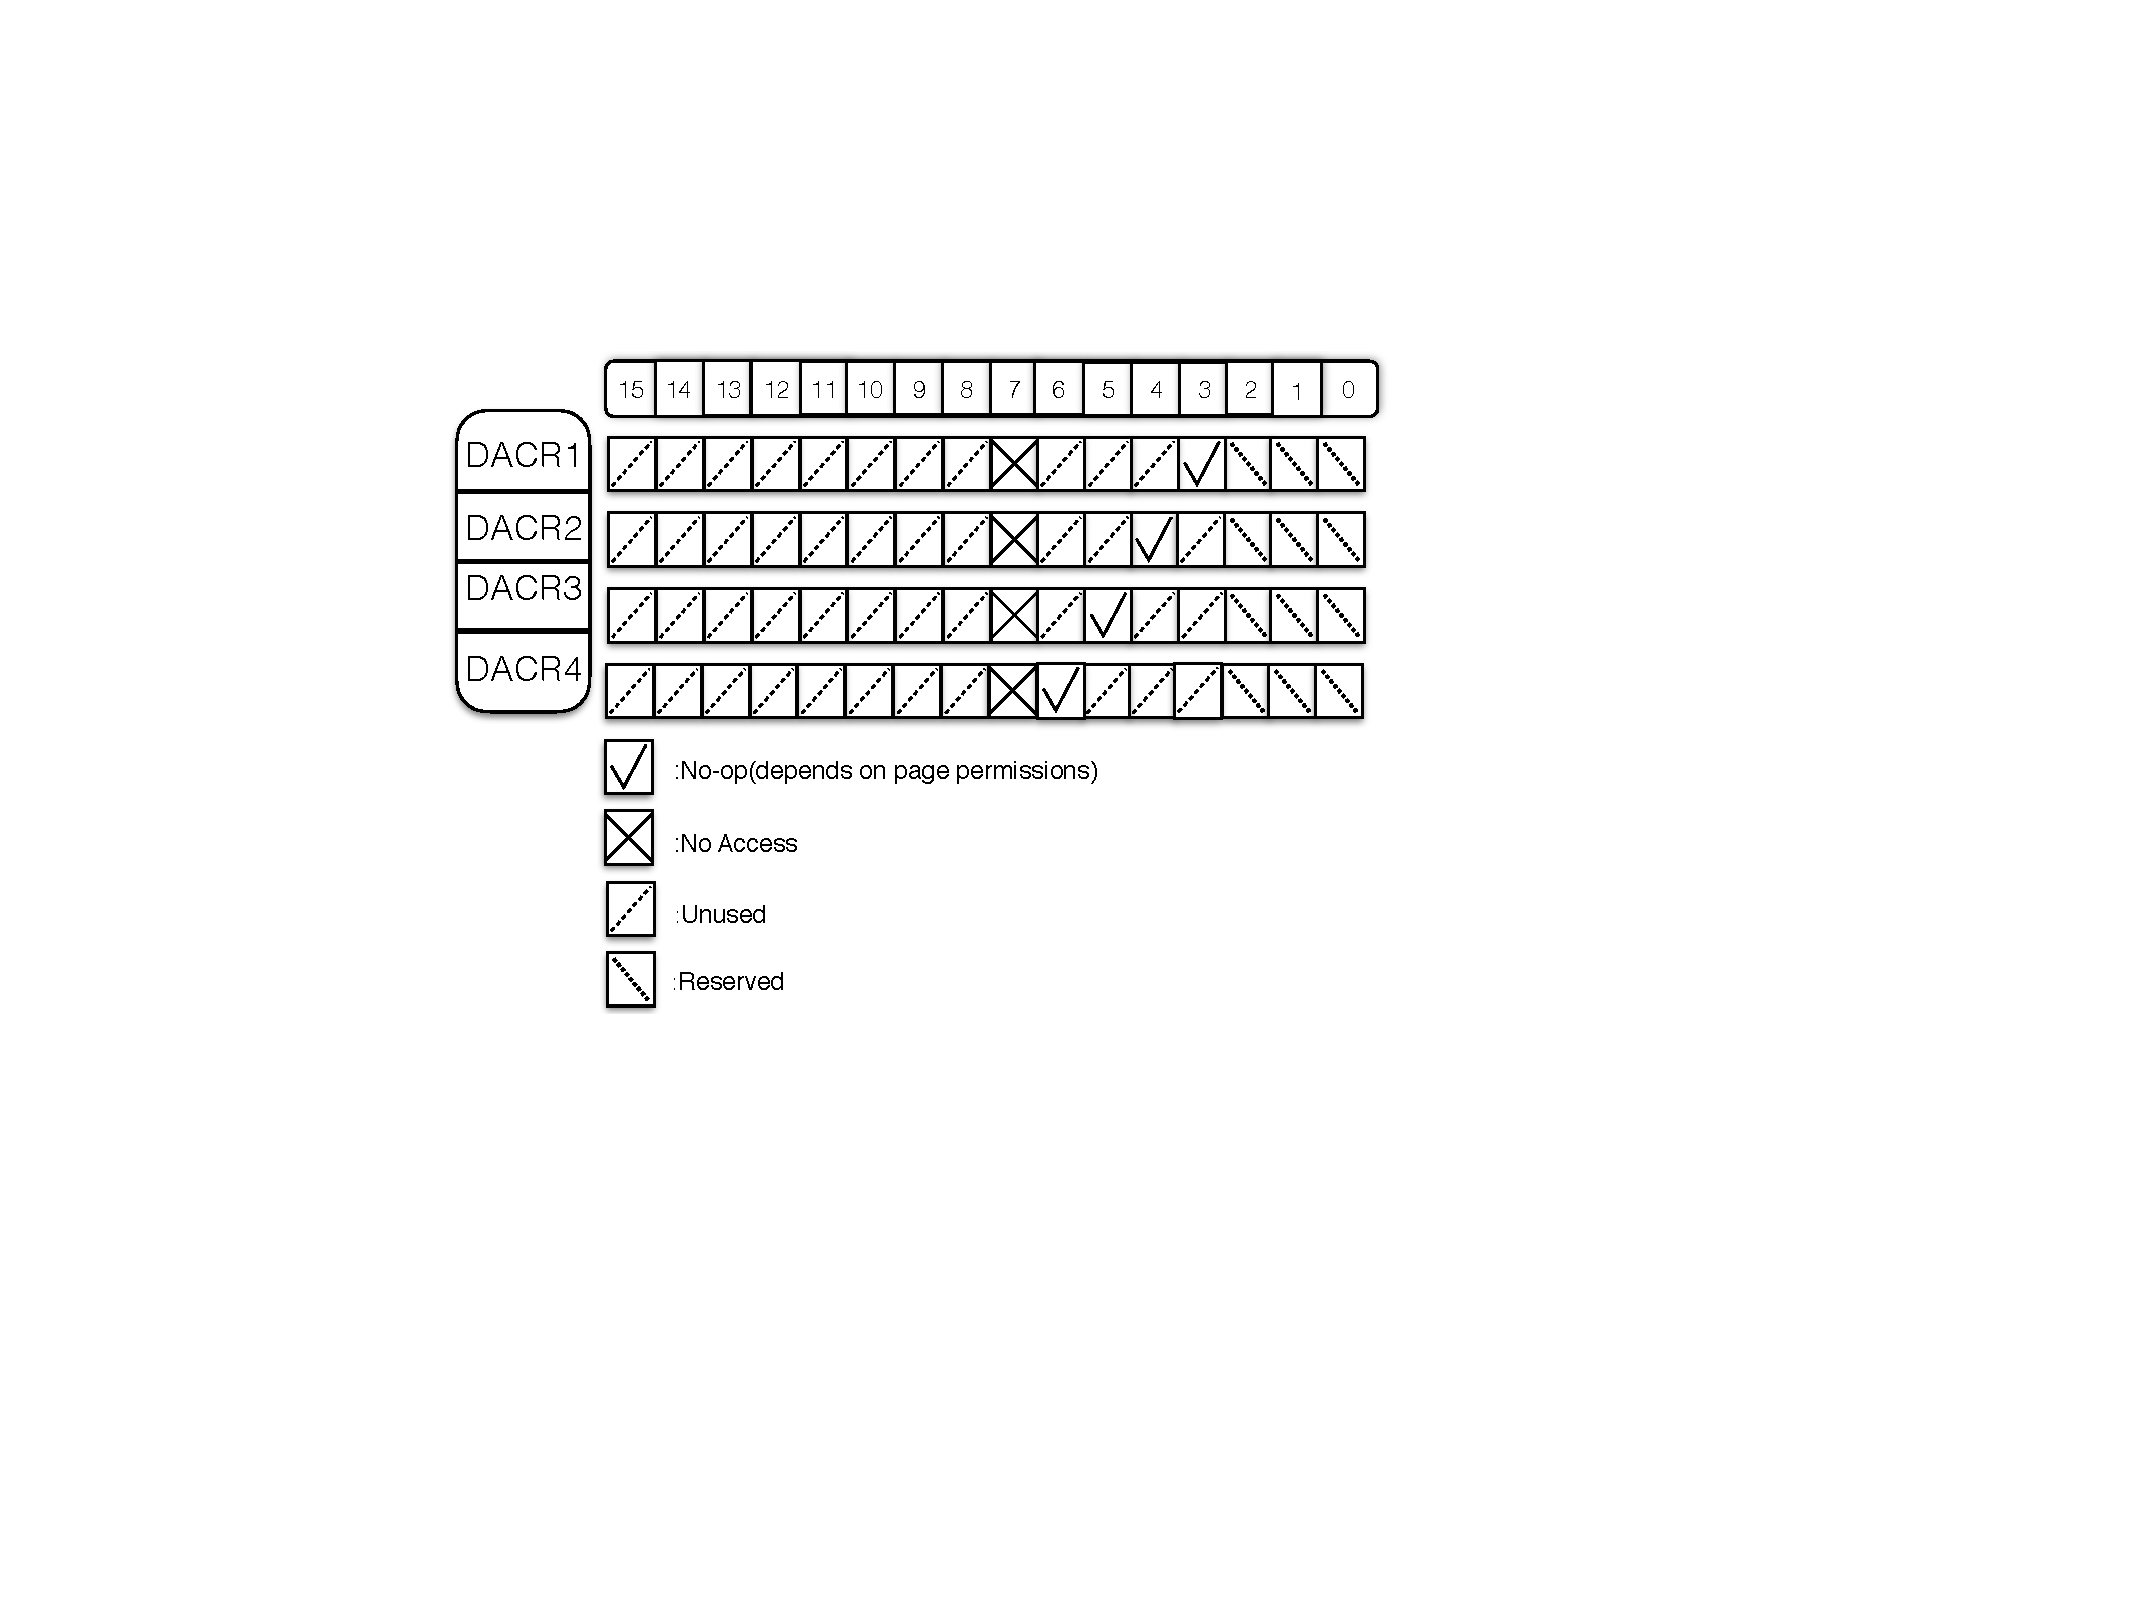
\includegraphics[width=\textwidth]{shreds/figures/dacr}
		\caption{The DACR setup for a quad-core system, where $k=4$. The first 3 domains ($Dom_{0}-Dom_{2}$) are reserved by Linux. Each core has a designated domain ($Dom_{3}-Dom_{6}$) that it may access when executing a shred. No CPU can access $Dom_{7}$. 
		 }
		\label{fig:dacr_setup}
	\end{minipage}
 \hfill
	\begin{minipage}[b]{0.4\textwidth}
		\centering	
		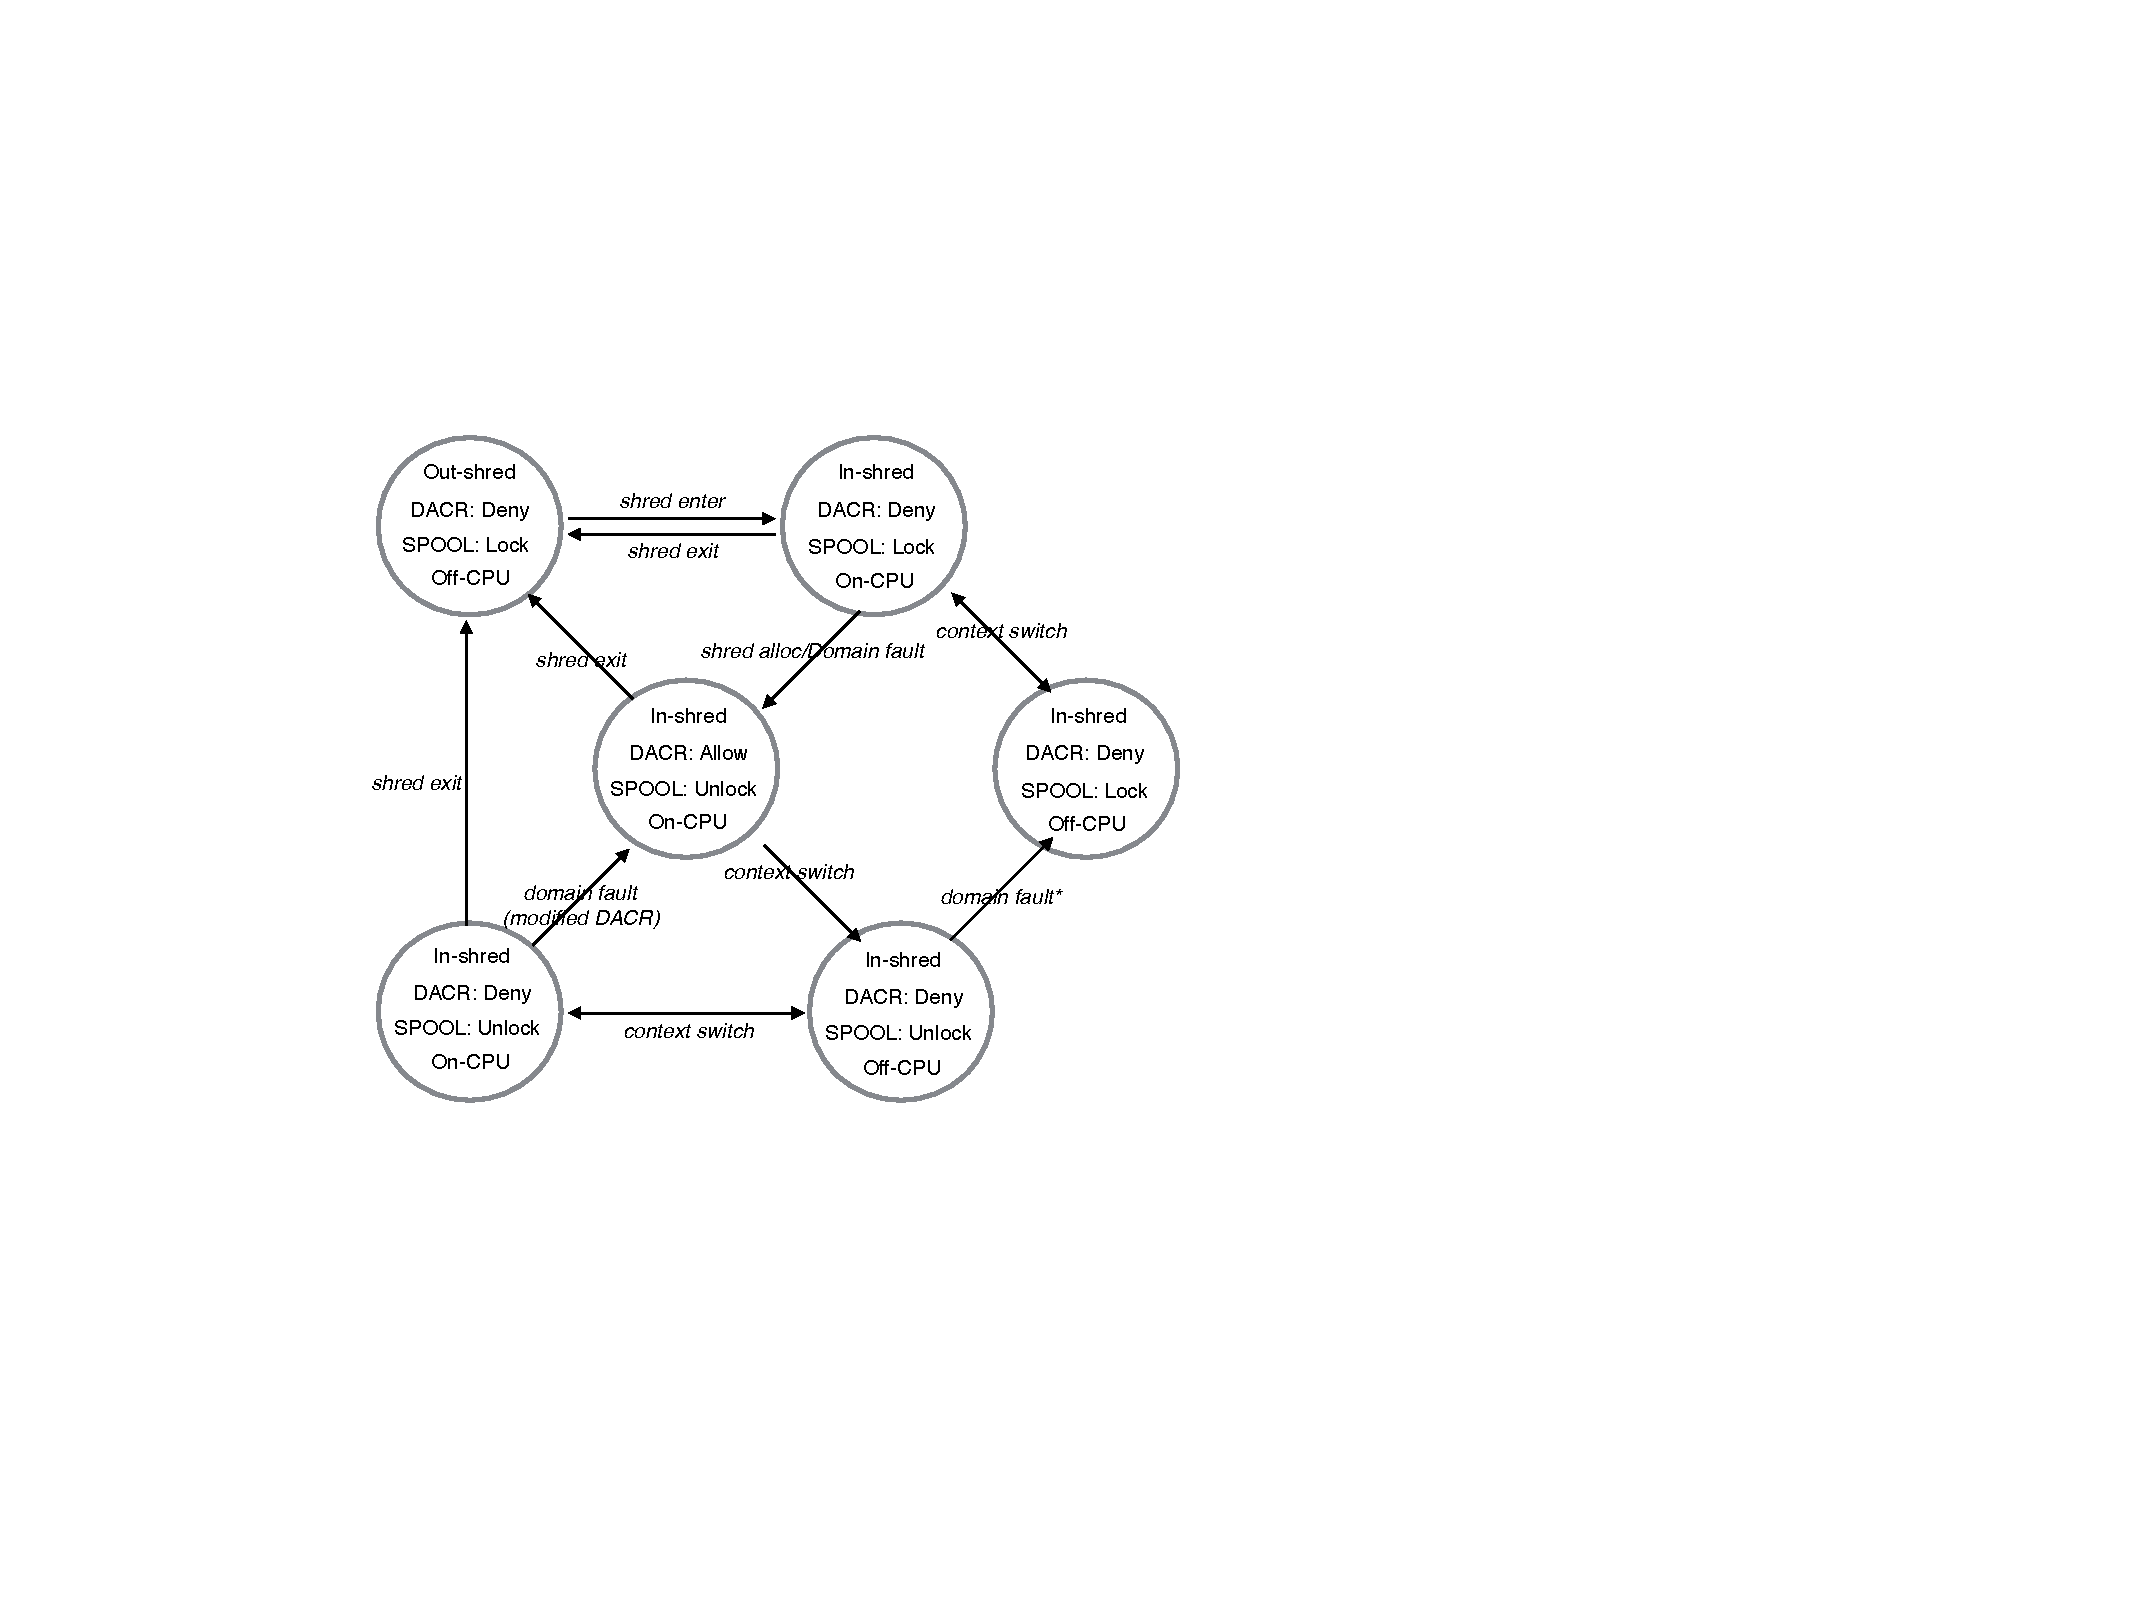
\includegraphics[width=\textwidth]{shreds/figures/shred_state_transition}
		\caption{A shred's transition of states}
		\label{fig:shredstat}
	\end{minipage}
\end{figure*}

S-driver uses the $k$ CPUs and the $k+1$ domains for executing shreds and protecting s-pools. 
When a shred starts or resumes its execution on $CPU_{i}$, S-driver assigns its associated s-pool to $Dom_{i}$, and therefore, the shred can freely access its s-pool while other concurrent threads, if any, cannot. 
When the shred terminates or is preempted, S-driver assigns its s-pool to $Dom_{k+1}$, which prevents any access to the pool from that moment on. 
As a result, S-driver allows or denies access to s-pools on a per-CPU basis, depending on if an associated shred occupies the CPU. 
Even if any malicious code manages to run concurrently alongside the shred inside the same process on another CPU, it cannot access the shred's s-pool without triggering domain faults. Thus, $P1$ is achieved. 

% performance and optimization 
It is reasonably efficient to switch s-pools to different domains upon shred entries and exits are. These operations do not involve heavy page table switches as process- or VM-based solutions do. They only require a shallow walk through of the first level page table and updates to the PDEs pointing to the s-pools in question. Besides, they do not trigger full TLB flushes as our design uses the per-address TLB eviction interface ({\tt flush\_tlb\_page}) and only invalidates the TLB entries related to the updated PDEs. 
To further reduce the overhead, we invent a technique called {\em lazy domain adjustment}: when a shred is leaving $CPU_{i}$, without adjusting any domain assignment, S-driver quickly changes the DACR to revoke the CPU's access to $Dom_{i}$ and lets the CPU's execution continue. It does not assign the s-pool used by the previous shred to $Dom_{k+1}$ until a domain fault happens (\ie another shred coming to the CPU and accessing its s-pool). The lazy domain adjustment avoids unnecessary domain changes and halves the already small overhead in some test cases.

%\begin{figure}[t]
%\begin{center}
%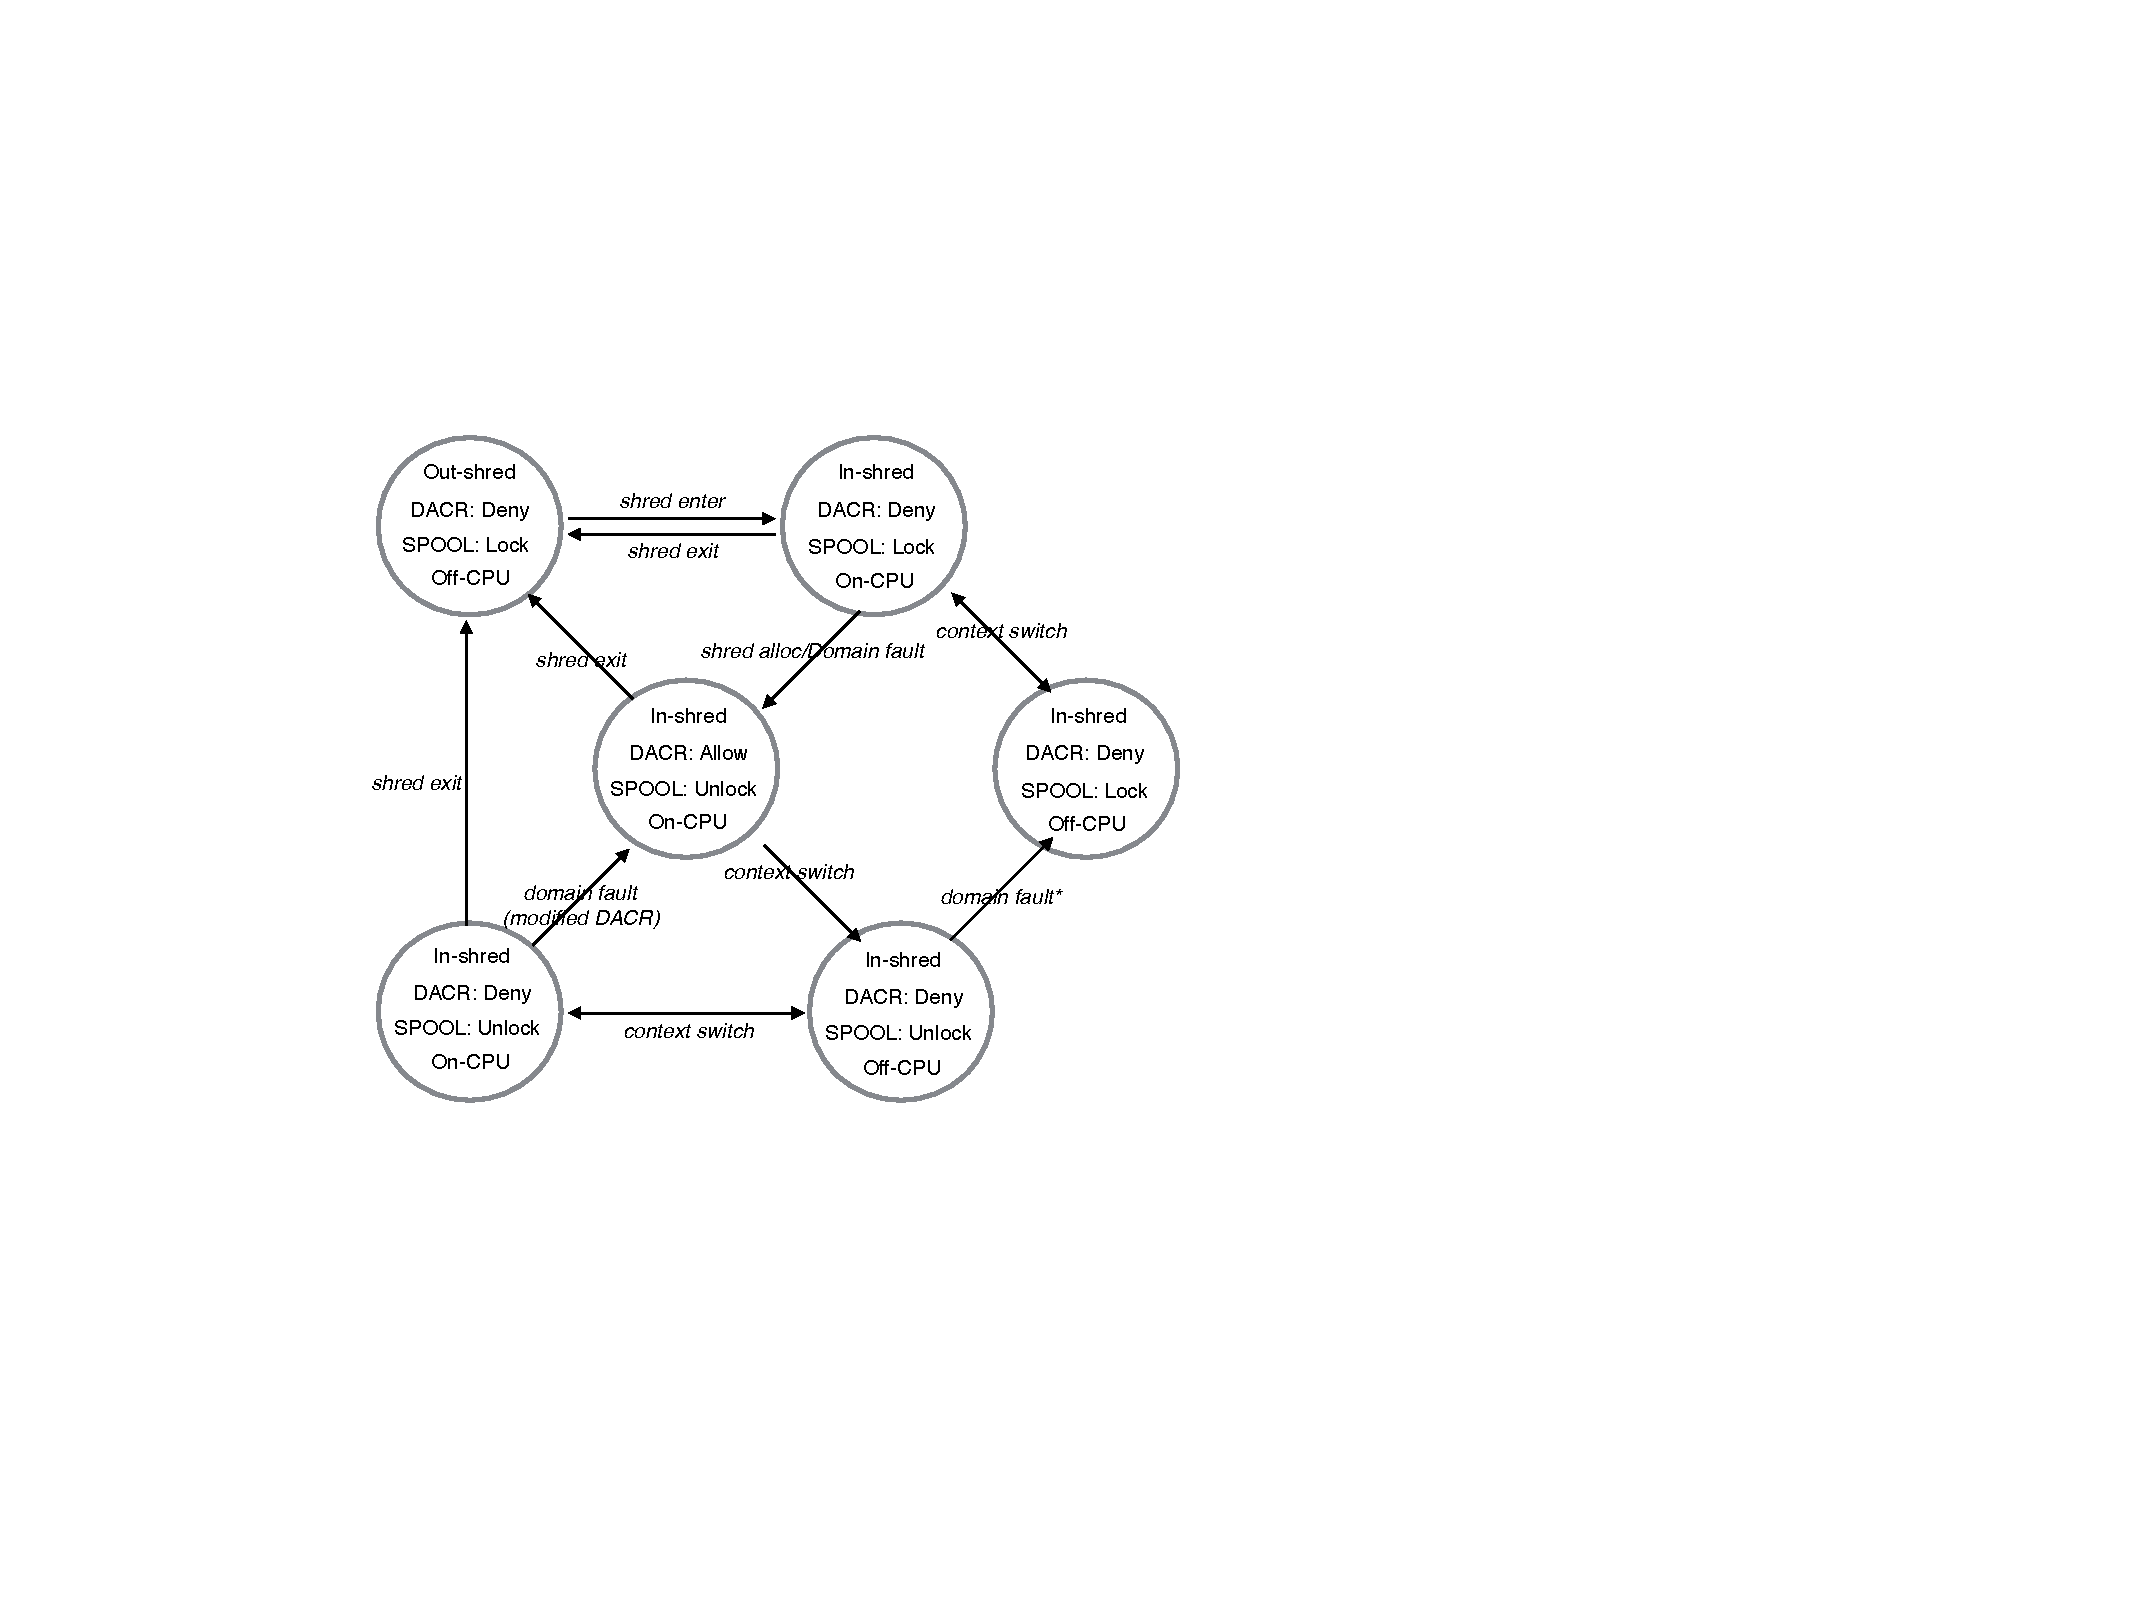
\includegraphics[scale=0.65]{shreds/figures/shred_state_transition}
%\caption{A shred's transition of states}
%\label{fig:shredstat}
%\end{center}
%\end{figure}

Figure~\ref{fig:shredstat} shows how S-driver orchestrates the transitions of a shred's states in response to the API calls, context switches, and domain faults. Each state is defined by a  combination of four properties:  

\begin{itemize}
\item $Shred$ = \{In-shred $|$ Out-shred\}: if the shred has started or exited. 
\item $DACR$ = \{Allow $|$ Deny\}: if the DACR allows or denies the current CPU to access its domain. 
\item $SPOOL$ = \{Lock $|$ Unlock\}: if the associated s-pool is locked or not. 
\item $CPU$ = \{On-CPU $|$ Off-CPU\}: if the shred is running on a CPU or not. 
\end{itemize}

The transition starts from the top, left circle, when the shred has not started and its s-pool is locked. After {\tt shred\_enter} is called, S-driver starts the shred, but it will not adjust the DACR or the s-pool access till a domain fault or a {\tt spool\_alloc} call due to the lazy domain adjustment in effect. When a context switch happens in the middle of the shred execution with unlocked DACR and s-pool, S-driver instantly sets the DACR to Deny but (safely) leaves the s-pool open. Later on, if a domain fault occurs, S-driver locks the previous s-pool because the fault means that the current code running on the CPU is in-shred and is trying to access its s-pool. If a domain fault never occurs till the shred regains the CPU, S-driver does not need to change any domain or s-pool settings, in which case the lazy domain adjustment saves two relatively heavy s-pool locking and unlocking operations. 
 
\point{Secure stacks for shreds}
%shadow stack support and switch 
Although S-compiler forbids unsanitized data flows from s-pools to unprotected memory regions, it has to allow in-shred code to copy s-pool data to local variables, which would be located in the regular stack and potentially accessible to in-process malicious code. 
To prevent secret leaks via stacks, S-driver creates a secure stack for each shred, allocated from its associated s-pool. When code execution enters a shred, S-driver transparently switches the stack without the application's knowledge: it copies the current stack frame to the secure stack and then overwrites the stack pointer. When the shred exits or encounters a signal to be handled outside of the shred, S-driver restores the regular stack.
As a result, local variables used by shreds never exist in regular stacks, and therefore cannot leak secrets.

\point{Runtime protection of shreds}
In addition to enabling and securing shreds and s-pools, S-driver also protects the inline reference monitor (IRM) that S-compiler plants in shred code. 
S-driver write-protects the memory pages containing the instrumented code and the associated data in memory.
It also pins the pages in s-pools in memory to prevent leaks via memory swap.  
Given that our threat model assumes the existence of in-process adversaries, S-driver also mediates the system calls that malicious code in user space may use to overwrite the page protection, dump physical memory via {\tt /dev/*mem}, disturb shreds via {\tt ptrace}, or load untrusted kernel modules. 
For each program using shreds, S-driver starts this mediation before loading the program code, avoiding pre-existing malicious code. 

S-driver's system call mediation also mitigates the attacks that steal secret data, not directly from s-pools, but from the I/O media where secret data are loaded or stored. 
For instance, instead of targeting the private key loaded in an s-pool, an in-process attacker may read the key file on disk. 
S-driver monitors file-open operations insides shreds. When the first time a file $F$ is accessed by a shred $S$, S-driver marks $F$ as a shred-private file and only allows shreds that share the same s-pool with $S$ to access $F$. This restriction is persistent and survives program and system reboots. 
As a result, an attacker can read $F$ only if she manages to intrude the program during its first run and access $F$ before a shred does. Although not completely preventing such attacks, S-driver makes them very difficult to succeed in reality. 
For a complete remedy, we envision a new primitive for in-shred code to encrypt and decrypt secret data with a persistent key assigned to each s-pool and automatically managed by S-driver. However, our current prototype does not support this primitive. 


It is worth noting that, although the system call mediation can prevent user-space malicious code that tries to break shreds via the system interfaces, it is a more intrusive and less configurable design choice than the well-known access control and capability frameworks, such as SELinux, AppArmor, and Capsicum~\cite{watson2010capsicum}. 
However, we leave the integration with those systems as future work because the system call mediation is easy to implement and is sufficient for the prototyping purpose. 



\subsection{Implementation}
\label{shreds:sec:impl}

We built S-compiler based on LLVM~\cite{lattner2004llvm} and its C front-end  Clang~\cite{clang}. We built S-driver with Linux as the reference OS. The implemented system was deployed and evaluated on a quad-core ARM Cortex-A7 computer (Raspberry Pi 2 Model B running Linux 4.1.15).

\point{S-compiler}
The modular and pass-based architecture of LLVM allows us to take advantage of the existing analyzers and easily extends the compilation pipeline. 
S-compiler adds two new passes to LLVM: the shred analysis pass and the security instrumentation pass. Both operate on LLVM bitcode as the IR. 

The analysis pass carries out the checks on the usages and security properties of shreds, as described in \S~\ref{shreds:sec:design}. 
We did not use LLVM's built-in data flow analysis for those checks due to its overly heuristic point-to analysis and the unnecessarily conservative transfer functions.
Instead, we implemented our specialized data flow analysis based on the basic round-robin iterative algorithm, with weak context sensitivity and a straightforward propagation model (i.e., only tracking value-conserving propagators).
We also had to extend LLVM's compilation pipeline because it by default only supports intra-module passes while S-compiler needs to perform inter-module analysis. We employed a linker plugin, called the Link-Time Optimization (LTO), to cross link the IR of all compilation modules and feed the linked IR to our analyzers. 


The instrumentation pass uses the LLVM IR Builder interfaces to insert security checks into the analyzed IR, which are necessary for enforcing the in-shred control flow regulations and preventing dynamic data leaks. 

\IncMargin{1em}
\begin{algorithm}
\small
\SetKwData{Spool}{s\_pool}
\SetKwData{Owner}{s\_owner}
\SetKwData{FaultThread}{fault\_thread}
\SetKwData{CPUDomain}{cpu\_domain}
\SetKwData{SpoolDomain}{s\_pool\_domain}
\SetKwFunction{FindSpool}{FindSpool}
\SetKwFunction{GetOwner}{GetOwner}
\SetKwFunction{GetCPUDomain}{GetCPUDomain}
\SetKwFunction{GetSpoolDomain}{GetSpoolDomain}
\SetKwFunction{BadArea}{bad\_area}
\SetKwFunction{GoodArea}{good\_area}
\SetKwFunction{RestoreDACR}{RestoreDACR}
\SetKwFunction{UnlockSPool}{UnlockSPool}
\SetKwFunction{AdjustSPool}{AdjustSPool}
\SetKwFunction{LockActiveSPoolList}{LockOtherActiveSPools}
\SetKwInOut{Input}{input}
\SetKwInOut{Output}{result}
\Input{The faulting virtual address $fault\_addr$}
\Output{Recover from the domain fault, or kill the faulting thread}
\BlankLine
\emph{/*Identity check*/}\\
  \Spool$\leftarrow$ \FindSpool{$fault\_addr$}\;
  \Owner$\leftarrow$ \GetOwner{$\Spool$}\;
  \If{\FaultThread is NOT in shred}{goto \BadArea}
  \If{\FaultThread is NOT \Owner}{goto \BadArea}
\BlankLine
\emph{/*Recover from domain fault*/}\\
  \CPUDomain$\leftarrow$ \GetCPUDomain{}\;
  \SpoolDomain$\leftarrow$ \GetSpoolDomain{\Spool}\;
   \If{\Spool is unlocked}
   {
   		  
          \If{\CPUDomain $=$ \SpoolDomain}
          {
            \emph{/*No need to change domain for s\_pool*/} \\
            \RestoreDACR{}\;
          }
          \Else
   		  {
   		    \AdjustSPool{\CPUDomain}  
   		  }
   }
    \Else
    {
    	\UnlockSPool{\CPUDomain} 
    }
   \LockActiveSPoolList{\Spool}\;
\caption{Domain Fault Handler}\label{dom_fault_handler}
\end{algorithm}
\DecMargin{1em}

\point{S-driver}
We built S-driver into a Loadable Kernel Module (LKM) for Linux. 
S-driver creates a virtual device file ({\tt /dev/shreds}) to handle the {\tt ioctl} requests made internally by the shred APIs. 
It uses 13 out of 16 memory domains to protect s-pools because the recent versions of Linux kernel for ARM already occupies 3 domains (for isolating device, kernel, and user-space memory). 
S-driver uses the available domains to protect unlimited s-pools and controls each CPU's access to the domains as described in \S~\ref{shreds:sec:design}.
Since Linux does not provide callback interfaces for drivers to react to scheduling events, in order to safely handle context switches or signal dispatches in shreds, 
S-driver dynamically patches the OS scheduler so that, during every context switch, the DACR of the current CPU is reset, which locks the open s-pool, if any. 
The overhead of this operation is negligible because resetting the DACR only takes a single lightweight instruction. 
To capture illegal access to s-pools and lazily adjust domain assignments, 
S-driver registers itself to be the only handler of domain faults and is triggered whenever a domain violation happens. 
Algorithm~\ref{dom_fault_handler} shows how S-driver handles a domain fault. 
Purely implementing S-driver as a LKM allows shreds to be introduced into a host without installing a custom-build kernel image.


\subsection{Analysis}
\label{rpo:sec:analysis}

% \begin{table}[t]
    \caption{Narrowing down the Common Crawl to the candidate set used in our analysis (from left to right).}
    \label{rpo:tab:dataset_stats}
    \centering
    \footnotesize
    \begin{tabular}{lrrr}
    \toprule
    \multicolumn{2}{r}{\textbf{Relative CSS}} & \textbf{Alexa Top 1M} & \textbf{Candidate Set} \\
    \midrule
    All Pages & 203,609,675 & 141,384,967 & 136,793,450 \\
    Tested Pages & 53,725,270 & 31,448,446 & 30,991,702 \\
    Sites & 5,960,505 & 223,212 & 222,443 \\
    Document Types & 9,833 & 2,965 & 2,898 \\
    \bottomrule
    \end{tabular}
\end{table}


For the purposes of our analysis, we gradually narrow down the seed data from
the Common Crawl to pages using relative style paths in the Alexa Top 1\,M,
reflecting injected style directives under RPO, and being exploitable due to
quirks mode rendering.

% Table~\ref{rpo:tab:dataset_stats} shows a summary of our dataset. \textit{Tested
% Pages} refers to the set of randomly selected pages from the page groups as
% discussed in Section~\ref{rpo:sec:methodology:candidate}. For brevity,
% we are referring to \textit{Tested Pages} wherever we mention pages in the
% remainder of the paper.

\subsubsection{Relative Stylesheet Paths}
\label{rpo:sec:analysis:relative}

\begin{figure}[t]
\centering
\begin{minipage}{.32\textwidth}
    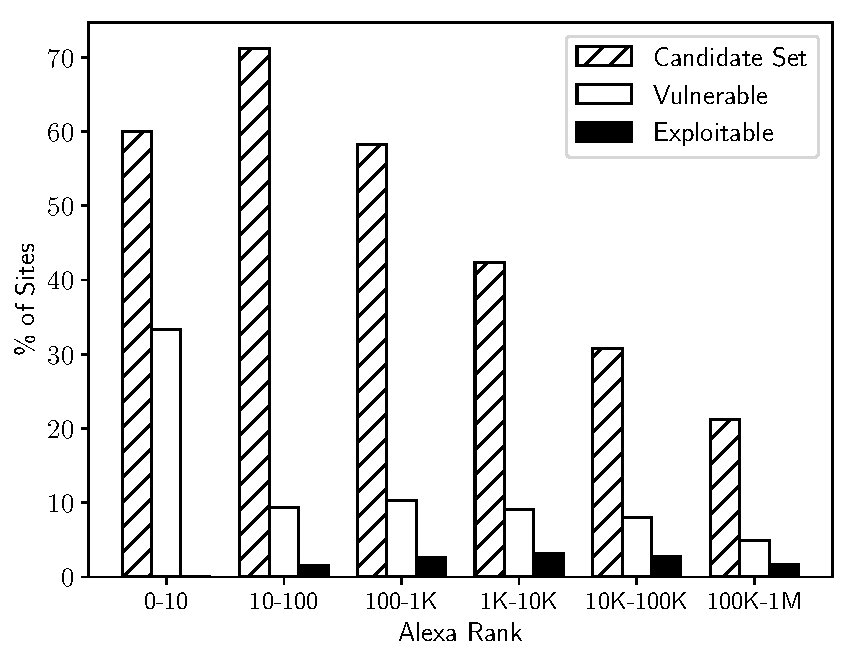
\includegraphics[width=1\textwidth,height=.8\textwidth]{rpo/figures/alexa_rank}
    \caption{Percentage of the Alexa site ranking in our candidate set
             (exponentially increasing bucket size).}
    \label{rpo:fig:analysis:alexa_rank}
\end{minipage}
\hfill
\begin{minipage}{.32\textwidth}
    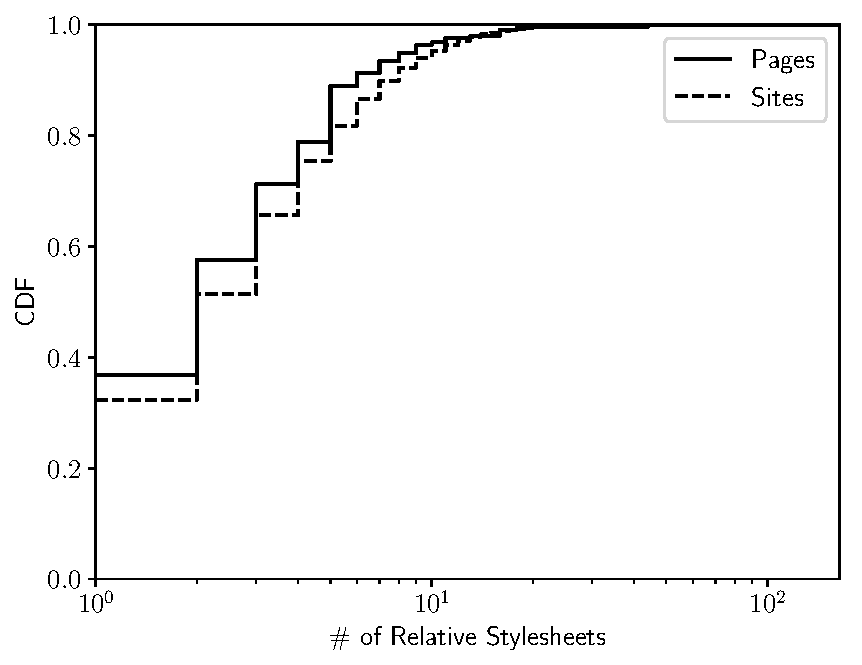
\includegraphics[width=1\textwidth,height=.8\textwidth]{rpo/figures/relative_stylesheets}
    \caption{CDF of total and maximum number of relative stylesheets per web
             page and site, respectively.}
    \label{rpo:fig:analysis:relative_stylesheets}
\end{minipage}
\hfill
\begin{minipage}{.32\textwidth}
    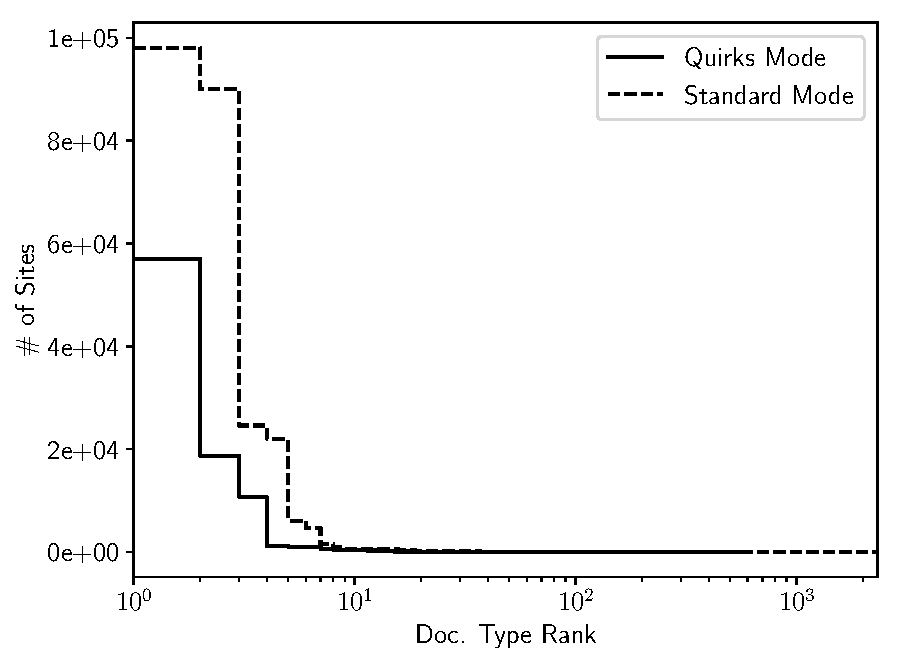
\includegraphics[width=1\textwidth,height=.8\textwidth]{rpo/figures/doctypes_rank_sites}
    \caption{Number of sites containing at least one page with a certain
             document type (ordered by doctype rank).}
    \label{rpo:fig:analysis:doctypes_rank_sites}
\end{minipage}
\end{figure}


To assess the extent to which our Common Crawl-seeded candidate set covers sites
of different popularity, consider the hatched bars in
Figure~\ref{rpo:fig:analysis:alexa_rank}. Six out of the ten largest sites
according to Alexa are represented in our candidate set. That is, they are
contained in the Common Crawl, and have relative style paths. The figure shows
that our candidate set contains a higher fraction of the largest sites and a
lower fraction of the smaller sites. Consequently, our results better represent
the most popular sites, which receive most visitors, and most potential victims
of RPO attacks.

While all the pages in the candidate set contain at least one relative
stylesheet path, Figure~\ref{rpo:fig:analysis:relative_stylesheets} shows that
63.1\,\% of them contain multiple relative paths, which increases the chances of
finding a successful RPO and style injection point.

\subsubsection{Vulnerable Pages}
\label{rpo:sec:analysis:vulnerable}

\begin{table*}[t]
    \centering
    \caption{Vulnerable/exploitable pages and sites in the candidate set (IE using framing).}
    \label{rpo:tab:vulnerable_exploitable_result}
    \footnotesize
    \begin{tabular}{lrrrrrr}
    \toprule
    \multirow{2}{*}{\textbf{Technique}} &
    \multicolumn{2}{c}{\textbf{Vulnerable}} &
    \multicolumn{2}{c}{\textbf{Exploitable (Chrome)}} &
    \multicolumn{2}{c}{\textbf{Exploitable (IE)}} \\

    \cmidrule[0.5pt](lr){2-3}
    \cmidrule[0.5pt](lr){4-5}
    \cmidrule[0.5pt](lr){6-7}

    &
    \textbf{Pages} &
    \textbf{Sites} &
    \textbf{Pages} &
    \textbf{Sites} &
    \textbf{Pages} &
    \textbf{Sites}
    \\

    \midrule

    Path Parameter & 309,079 (1.0\%) & 9,136 (4.1\%) & 6,048 (\textless 0.1\%) & 1,025 (0.5\%) & 52,344 (0.2\%) & 3,433 (1.5\%) \\
    Encoded Path & 53,502 (0.2\%) & 1,802 (0.8\%) & 3 (\textless 0.1\%) & 2 (\textless 0.1\%) & 24 (\textless 0.1\%) & 5 (\textless 0.1\%) \\
    Encoded Query & 89,757 (0.3\%) & 1,303 (0.6\%) & 23 (\textless 0.1\%) & 20 (\textless 0.1\%) & 137 (\textless 0.1\%) & 43 (\textless 0.1\%) \\
    Cookie & 15,656 (\textless 0.1\%) & 1,030 (0.5\%) & 4,722 (\textless 0.1\%) & 81 (\textless 0.1\%) & 2,447 (\textless 0.1\%) & 238 (0.1\%) \\

    \midrule

    Total & 377,043 (1.2\%) & 11,986 (5.4\%) & 10,781 (<0.1\%) & 1,106 (0.5\%) & 54,853 (0.2\%) & 3,645 (1.6\%) \\

    \bottomrule
    \end{tabular}

\end{table*}


We consider a candidate page vulnerable if one of the style injection techniques
of Section~\ref{rpo:sec:methodology:vulnerable} succeeds. In other
words, the server's response should reflect the injected payload. Furthermore,
we conservatively require that the response not contain a \texttt{base} tag
since a correctly configured base tag can prevent path confusion.

Table~\ref{rpo:tab:vulnerable_exploitable_result} shows that 1.2\,\% of pages
are vulnerable to at least one of the injection techniques, and 5.4\,\% of sites
contain at least one vulnerable page. The path parameter technique is most
effective against pages, followed by the encoded query and the encoded path
techniques. Sites that are ranked higher according to Alexa are more likely to
be vulnerable, as shown in Figure~\ref{rpo:fig:analysis:alexa_rank}, where
vulnerable and exploitable sites are relative to the candidate set in each
bucket. While one third of the candidate set in the Top~10 (two out of six
sites) is vulnerable, the percentage oscillates between 8 and 10\,\% among the
Top~100\,k. The candidate set is dominated by the smaller sites in the ranks
between 100\,k and 1\,M, which have a vulnerability rate of 4.9\,\% and push
down the average over the entire ranking.

% A \texttt{base} tag in the server response can prevent path confusion because it
% indicates how the browser should expand relative paths. We observed a number of
% inconsistencies with respect to its use. At first, 603 pages on 60 sites
% contained a \texttt{base} tag in their response; however, the server response
% after injecting our payload did not contain the tag anymore, rendering these
% pages potentially exploitable. Furthermore, Internet Explorer's implementation
% of the \texttt{base} tag appears to be broken. When such a tag is present,
% Internet Explorer fetches two URLs for stylesheets---one expanded according to
% the base URL specified in the tag, and one expanded in the regular, potentially
% ``confused'' way of using the page URL as the base. In our experiments, Internet
% Explorer always applied the ``confused'' stylesheet, even when the one based on
% the \texttt{base} tag URL loaded faster. Consequently, \texttt{base} tags do not
% appear to be an effective defense against RPO in Internet Explorer (They seem to
% work as expected in other browsers, including Edge).


\subsubsection{Exploitable Pages}
\label{rpo:sec:analysis:exploitable}

To test whether a vulnerable page was exploitable, we opened it in Chrome,
injected a style payload with an image reference (randomly generated URL), and
checked if the image was indeed loaded. This test succeeded for 2.9\,\% of
vulnerable pages; 0.5\,\% of sites in the candidate set had at least one
exploitable page (Table~\ref{rpo:tab:vulnerable_exploitable_result}).

% In the following, we explore various factors that may impact whether a
% vulnerable page can be exploited, and we show how some of these partial defenses
% can be bypassed.

% \paragraph{Document Types}
% \label{rpo:sec:analysis:doctypes}

% \begin{table}[t]
\centering
\begin{minipage}[t]{.55\textwidth}
    \caption{Summary of document type usage in sites.\newline}
    \label{rpo:tab:doctypes_summary}
    \centering
    \footnotesize
    \begin{tabular}{lrr}
    \toprule
    \textbf{Doc. Type} & \textbf{At Least One Page} & \textbf{All Pages} \\
    \midrule

    None & 56,985 (25.6\%) & 19,968 (9.0\%) \\
    Quirks & 27,794 (12.5\%) & 7,720 (3.5\%) \\
    None or Quirks & 71,597 (32.2\%) & 30,040 (13.5\%) \\
    \addlinespace
    Standards & 192,403 (86.5\%) & 150,846 (67.8\%) \\    
    \bottomrule
    \end{tabular}
\end{minipage}
\hfill
\begin{minipage}[t]{.43\textwidth}
    \caption{Quirks mode document types by browser.}
    \label{rpo:tab:doctypes_browsers}
    \centering
    \footnotesize
    \begin{tabular}{llr}
    \toprule

    \textbf{Browser} &
    \textbf{OS} &
    \textbf{Doc. Types} \\

    \midrule
    Chrome 55 & Linux & 1,378 (31.9\,\%) \\
    Opera 42 & Linux & 1,378 (31.9\,\%) \\
    Safari 10 & macOS & 1,378 (31.9\,\%) \\
    \addlinespace
    Firefox 50 & Linux & 1,326 (30.7\,\%) \\
    \addlinespace
    Edge 38 & Windows & 1,319 (30.5\,\%) \\
    IE 11 & Windows & 1,319 (30.5\,\%) \\
    \bottomrule
    \end{tabular}
\end{minipage}
\end{table}


% \begin{table}[t]
    \caption{Most frequent document types causing all browsers to render
    in quirks mode, as well as the sites that use at least one such
    document type.}
    \label{rpo:tab:top_quirksmode_doctypes}
    \centering
    \footnotesize
    \begin{tabular}{lrr}
    \toprule
    \textbf{Document Type (shortened)} & \textbf{Pages} & \textbf{Sites} \\
    \midrule
    (none) & 1,818,595 (5.9\,\%) & 56,985 (25.6\,\%) \\
    "-//W3C//DTD HTML 4.01 Transitional//EN" & 721,884 (2.3\,\%) & 18,648 (8.4\,\%) \\
    "-//W3C//DTD HTML 4.0 Transitional//EN" & 385,656 (1.2\,\%) & 11,566 (5.2\,\%) \\
    "-//W3C//DTD HTML 3.2 Final//EN" & 22,019 (<0.1\,\%) & 1,175 (0.5\,\%) \\
    "-//W3C//DTD HTML 3.2//EN" & 10,839 (<0.1\,\%) & 927 (0.4\,\%) \\
    \midrule
    All & 3,046,449 (9.6\,\%) & 71,597 (32.2\,\%) \\
    \bottomrule
    \end{tabular}
\end{table}


% HTML document types play a significant role in RPO-based style injection attacks
% because browsers typically parse resources with a non-CSS content type in a CSS
% context only when the page specifies an ancient or non-standard HTML document
% type (or none at all). The pages in our candidate set contain a total of 4,318
% distinct document types. However, the majority of these unique document types
% are not standardized and differ from the standardized ones only by small
% variations, such as forgotten spaces or misspellings.

% To determine how browsers interpret these document types (i.e., whether they
% cause them to render a page in standards or quirks mode), we designed a
% controlled experiment. For each unique document type, we set up a local page
% with a relative stylesheet path and carried out an RPO attack to inject CSS
% using a payload similar to what we described in
% Section~\ref{rpo:sec:methodology:vulnerable}. We automatically opened
% the local page in Chrome, Firefox, Edge, Internet Explorer, Safari, and Opera,
% and we kept track of which document type caused the injected CSS to be parsed
% and the injected background image to be downloaded.

% Table~\ref{rpo:tab:doctypes_browsers} contains the results of this experiment.
% Even though the exact numbers vary among browsers, roughly a third of the unique
% document types we encountered result in quirks mode rendering. Not surprisingly,
% both Microsoft products Edge and Internet Explorer exhibit identical results,
% whereas the common Webkit ancestry of Chrome, Opera, and Safari also show
% identical results. Overall, 1,271 (29.4\,\%) of the unique document types force
% all the browsers into quirks mode, whereas 1,378 (31.9\,\%) of them cause at
% least one browser to use quirks mode rendering.
% Table~\ref{rpo:tab:top_quirksmode_doctypes} shows the most frequently used
% document types that force all the browsers into quirks mode, which includes the
% absence of a document type declaration in the page.

% To test how often Internet Explorer allows a page's document type to be
% overridden when loading it in an \texttt{iframe}, we created another controlled
% experiment using a local attack page framing the victim page, as outlined in
% Section~\ref{rpo:sec:methodology:exploitable}. Using Internet
% Explorer~11, we loaded our local attack page for each unique document type
% inside the frame, and tested if the injected CSS was parsed. While Internet
% Explorer parsed the injected CSS for 1,319 (30.5\,\%) of the document types in
% the default setting, the frame override trick caused CSS parsing for 4,248
% (98.4\,\%) of the unique document types.

% While over one thousand document types result in quirks mode, and around three
% thousand document types cause standards mode parsing, the number of document
% types that have been standardized is several orders of magnitude smaller. In
% fact, only a few (standardized) document types are used frequently in pages,
% whereas the majority of unique document types are used very rarely.
% Figure~\ref{rpo:fig:analysis:doctypes_rank_sites} shows that only about ten
% standards and quirks mode document types are widely used in pages and sites.
% Furthermore, only about 9.6\,\% of pages in the candidate set use a quirks mode
% document type; on the remaining pages, potential RPO style injection
% vulnerabilities cannot be exploited because the CSS would not be parsed (unless
% Internet Explorer is used). However, when grouping pages in the candidate set by
% site, 32.2\,\% of sites contain at least one page rendered in quirks mode
% (Table~\ref{rpo:tab:doctypes_summary}), which is one of the preconditions for
% successful RPO.

% \paragraph{Internet Explorer Framing}

% We showed above that by loading a page in a frame, Internet Explorer can be
% forced to disregard a standards mode document type that would prevent
% interpretation of injected style. To find out how often this technique can be
% applied for successful RPO attacks, we replicated our Chrome experiment in
% Internet Explorer, this time loading each vulnerable page inside a frame. Around
% 14.5\,\% of vulnerable pages were exploitable in Internet Explorer, five times
% more than in Chrome (1.6\,\% of the sites in the candidate set).

% Figure~\ref{rpo:fig:analysis:alexa_rank} shows the combined exploitability
% results for Chrome and Internet Explorer according to the rank of the site.
% While our methodology did not find any exploitable vulnerability on the six
% highest-ranked sites in the candidate set, between 1.6\,\% and 3.2\,\% of
% candidate sites in each remaining bucket were found to be exploitable. The
% highest exploitability rate occurred in the ranks 1\,k through 10\,k.

% Broken down by injection technique, the framing trick in Internet Explorer
% results in more exploitable pages for each technique except for cookie injection
% (Table~\ref{rpo:tab:vulnerable_exploitable_result}). One possible explanation
% for this difference is that the Internet Explorer crawl was conducted one month
% after the Chrome crawl, and sites may have changed in the meantime. Furthermore,
% we observed two additional impediments to successful exploitation in Internet
% Explorer that do not apply to Chrome. The framing technique is susceptible to
% frame-busting methods employed by the framed pages, and Internet Explorer
% implements an anti-MIME-sniffing header that Chrome appears to ignore. We
% analyze these issues below.

% \paragraph{Anti-Framing Techniques}

% Some sites use a range of techniques to prevent other pages from loading them in
% a frame~\cite{w2sp2010frame_busting}. One of these techniques is the
% \texttt{X-Frame-Options} header. It accepts three different values:
% \texttt{DENY}, \texttt{SAMEORIGIN}, and \texttt{ALLOW-FROM} followed by a
% whitelist of URLs.

% In the vulnerable dataset, 4,999 pages across 391 sites use this header
% correctly and as a result prevent the attack. However, 1,900 pages across 34
% sites provide incorrect values for this header, and we successfully attack 552
% pages on 2 sites with Internet Explorer.

% A related technique is the \texttt{frame-ancestors} directive provided by
% Content Security Policy. It defines a (potentially empty) whitelist of URLs
% allowed to load the current page in a frame, similar to \texttt{ALLOW-FROM}.
% However, it is not supported by Internet Explorer, thus it cannot be used to
% prevent the attack.

% Furthermore, developers may use JavaScript code to prevent framing of a page.
% Yet, techniques exist to bypass this
% protection~\cite{owasp_clickjacking_defence}. In addition, the attacker can use
% the HTML 5 \texttt{sandbox} attribute in the \texttt{iframe} tag and omit the
% \texttt{allow-top-navigation} directive to render JavaScript frame-busting code
% ineffective. However, we did not implement any of these techniques to allow
% framing, which means that more vulnerable pages could likely be exploited in
% practice.

% \paragraph{MIME Sniffing}

% A consequence of self-reference in the type of RPO studied in this paper is that
% the HTTP content type of the fake ``stylesheet'' is \texttt{text/html} rather
% than the expected \texttt{text/css}. Because many sites contain misconfigured
% content types, many browsers attempt to infer the type based on the request
% context or file extension (\textit{MIME sniffing}), especially in quirks mode.
% In order to ask the browser to disable content sniffing and refuse interpreting
% data with an unexpected or wrong type, sites can set the header
% \texttt{X-Content-Type-Options: nosniff}~\cite{sp2009contentsniff,firefox_mime_sniff,content_type_options}.

% To determine whether the injected CSS is still being parsed and executed in
% presence of this header while the browser renders in quirks mode, we ran an
% experiment similar to Section~\ref{rpo:sec:analysis:doctypes}. For each browser
% in Table~\ref{rpo:tab:doctypes_browsers}, we extracted the document types in
% which the browser renders in quirks mode, and for each of them, we set up a
% local page with a relative stylesheet path. We then opened the page in the
% browser, launched an RPO attack, and monitored if the injected CSS was executed.

% Only Firefox, Internet Explorer, and Edge respected this header and did not
% interpret injected CSS in any of the quirks mode document types. The remaining
% browsers did not block the stylesheet even though the content type was not
% \texttt{text/css}. With an additional experiment, we confirmed that Internet
% Explorer blocked our injected CSS payload when \texttt{nosniff} was set, even in
% the case of the framing technique.

% Out of all the vulnerable pages, 96,618 pages across 232 sites had a
% \texttt{nosniff} response header; 23 pages across 10 sites were confirmed
% exploitable in Chrome but not in Internet Explorer, since the latter browser
% respects the header while the former does not.

% \subsubsection{Content Management Systems}
% \label{rpo:sec:analysis:cmses}

% While analyzing the exploitable pages in our dataset, we noticed that many
% appeared to belong to well-known CMSes. Since these web applications are
% typically installed on thousands of sites, fixing RPO weaknesses in these
% applications could have a large impact.

% To identify CMSes, we visited all exploitable pages using
% Wappalyzer~\cite{wappalyzer}. Additionally, we detected two CMSes that were not
% supported by Wappalyzer. Overall, we identified 23 CMSes on 41,288 pages across
% 1,589 sites. Afterwards, we manually investigated whether the RPO weakness
% stemmed from the CMS by installing the latest version of each CMS (or using the
% online demo), and testing whether exploitable paths found in our dataset were
% also exploitable in the CMS. After careful analysis, we confirmed four CMSes to
% be exploitable in their most recent version that are being used by 40,255 pages
% across 1,197 sites.

% Out of the four exploitable CMSes, one declares no document type and one uses a
% quirks mode document type. These two CMSes can be exploited in Chrome, whereas
% the remaining two can be exploited with the framing trick in Internet Explorer.
% % Beyond the view of our Common Crawl candidate set, Wappalyzer detected nearly
% % 32\,k installations of these CMSes across the Internet, which suggests that many
% % more sites could be attacked with RPO. We reported the RPO weaknesses to the
% % vendors of these CMSes using recommended notification
% % techniques~\cite{usenixsec2016vulnnotify1,usenixsec2016vulnnotify2,weis2017vulnnotify}.
% % Thus far, we heard back from one of the vendors, who acknowledged the
% % vulnerability and are going to take the necessary steps to fix the issue.
% % However, we have not received any response from the other vendors.

% \subsubsection{Mitigation Techniques}
% \label{rpo:sec:mitigation}

% Relative path overwrites rely on the web server and the web browser interpreting
% URLs differently. HTML pages can use only absolute (or root-relative) URLs,
% which removes the need for the web browser to expand relative paths.
% Alternatively, when the HTML page contains a \texttt{<base>} tag, browsers are
% expected to use the URL provided therein to expand relative paths instead of
% interpreting the current document's URL.
% % Both methods can remove ambiguities and
% % render RPO impossible if applied correctly. Specifically, base URLs must be set
% % according to the server's content routing logic. If developers choose to
% % calculate base URLs dynamically on the server side rather than setting them
% % manually to constant values, there is a risk that routing-agnostic algorithms
% % could be confused by manipulated URLs and re-introduce attack opportunities by
% % instructing browsers to use an attacker-controlled base URL. Furthermore,
% % Internet Explorer does not appear to implement this tag correctly.
% % 
% Web developers can reduce the attack surface of their sites by eliminating any
% injection sinks for strings that could be interpreted as a style directive.
% % However, doing so is challenging because in the attack presented in this paper,
% % style injection does not require a specific sink type and does not need the
% % ability of injecting markup. Injection can be accomplished with relatively
% % commonly used characters, that is, alphanumeric characters and
% % \texttt{()\{\}/"}. Experience has shown that despite years of efforts, even
% % context-sensitive and more special character-intensive XSS injection is still
% % possible in many sites, which leads us to believe that style injection will be
% % similarly difficult to eradicate. Even when all special characters in user input
% % are replaced by their corresponding HTML entities and direct style injection is
% % not possible, more targeted RPO attack variants referencing existing files may
% % still be feasible. For instance, it has been shown that user uploads of
% % seemingly benign profile pictures can be used as ``scripts'' (or
% % stylesheets)~\cite{rpo_techniques}.

% Instead of preventing RPO and style injection vulnerabilities, the most
% promising approach could be to avoid exploitation. In fact, declaring a modern
% document type that causes the HTML document to be rendered in standards mode
% makes the attack fail in all browsers except for Internet Explorer. Web
% developers can harden their pages against the frame-override technique in
% Internet Explorer by using commonly recommended HTTP headers.
% % \texttt{X-Content-Type-Options} to disable ``content type sniffing'' and always
% % use the MIME type sent by the server (which must be configured correctly),
% % \texttt{X-Frame-Options} to disallow loading the page in a frame, and
% % \texttt{X-UA-Compatible} to turn off Internet Explorer's compatibility view.


\newcommand{\excision}{\textsc{Excision}\xspace}

\section{Detection of Malicious Third-Party Content Inclusions}

\subsection{Overview}
\label{inclusion:sec:overview}

While the same origin policy (SOP) enforces a modicum of origin-based separation
between code and data from different principals, developers have clamored for
more flexible sharing models provided by, e.g., Content Security Policy
(CSP)~\cite{csp_spec}, Cross-Origin Resource Sharing (CORS)~\cite{cors_spec},
and postMessage-based cross-frame communication. These newer standards permit
greater flexibility in performing cross-origin inclusions, and each come with
associated mechanisms for restricting communication to trusted origins. However,
recent work has shown that these standards are difficult to apply securely in
practice~\cite{ndss2013postman,raid2014csp}, and do not necessarily address the
challenges of trusting remote inclusions on the dynamic Web. In addition to the
inapplicability of some approaches such as CSP, third parties can leverage their
power to bypass these security mechanisms. For example, ISPs and browser
extensions are able to tamper with HTTP traffic to modify or remove CSP rules in
HTTP responses~\cite{usenixsec2015webeval,sp2015adinjection}.

In this section, we propose an in-browser approach called \excision to
automatically detect and block malicious third-party content inclusions as web
pages are loaded into the user's browser or during the execution of browser
extensions. Our approach does not rely on examination of the content of the
resources; rather, it relies on analyzing the sequence of inclusions that leads
to the resolution and loading of a terminal remote resource. Unlike prior
work~\cite{ccs2012madtracer}, \excision resolves \emph{inclusion sequences
(chains)} through instrumentation of the browser itself, an approach that
provides a high-fidelity view of the third-party inclusion process as well as
the ability to interdict content loading in real-time. This precise view also
renders ineffective common obfuscation techniques used by attackers to evade
detection. Obfuscation causes the detection rate of these approaches to degrade
significantly since obfuscated third-party inclusions cannot be traced using
existing techniques~\cite{ccs2012madtracer}. Furthermore, the in-browser
property of our system allows users to browse websites with a higher confidence
since malicious third-party content is prevented from being included while the
web page is loading.

We implemented \excision as a set of modifications to the Chromium browser, and
evaluated its effectiveness by analyzing the Alexa Top 200K over a period of 11
months. Our evaluation demonstrates that \excision achieves a 93.39\% detection
rate, a false positive rate of 0.59\%, and low performance overhead. We also
performed a usability test of our research prototype, which shows that \excision
does not detract from the user's browsing experience while automatically
protecting the user from the vast majority of malicious content on the Web. The
detection results suggest that \excision could be used as a complementary system
to other techniques such as CSP.




\subsection{Design}
\label{shreds:sec:design}
%We design and implement a system that enables shreds for Linux/ARM platforms. Our system consists of a compilation toolchain (S-compiler) and a dynamic loadable kernel extension (S-driver). Developers can adopt shreds in their programs using a set of simple APIs: two APIs for entering and exiting a shred; two APIs for allocating and freeing memory in an s-pool. S-compiler is needed to build programs that contain shreds. S-compiler performs the code analysis and instrumentation. During runtime, S-driver handles shred creations and terminations. It manages and protects s-pools. Our design makes a novel use of memory domains, an under-exploited feature in ARM CPUs, to efficiently protect s-pools and shred executions.
\subsubsection{Shred APIs and Usages}
Application developers use shreds and s-pools via the following intuitive APIs: 

\vspace{.1in}
\indent\indent {\tt err\_t }{\btt shred\_enter}{\tt (int {\itt pool\_desc})};   \\
\indent\indent {\tt err\_t }{\btt shred\_exit}{\tt ()};     \\
\indent\indent {\tt void * }{\btt spool\_alloc}{\tt (size\_t {\itt size})};   \\
\indent\indent {\tt void  }{\btt spool\_free}{\tt (void *{\itt ptr})};     
\vspace{.1in}

These APIs internally make requests to S-driver via {\tt ioctl} for managing shreds and s-pools.
To explain the API usage, we use the lightweight open-source web server, Lighttpd, as an example, where we employ shreds to protect the HTTP authentication password in Lighttpd's virtual memory. 
By wrapping the code that receives and checks the password in two shreds and storing the password in an s-pool, the modified Lighttpd prevents out-shred code, including third-party and injected code, from accessing the password in memory. 
Listings~\ref{list:request}-\ref{list:auth} show the code snippets that contain the  modifications (lines marked with ``+'').   

% enter shred
A successful call to {\btt shred\_enter} starts a shred execution on the current thread. 
It also causes a switch to a secure execution stack allocated in s-pool, which prevents potential secret leaks via local variables after the shred exits. 
The thread then is given exclusive access to the associated s-pool, which is specified by the developer using the {\itt pool\_desc} parameter of {\btt shred\_enter}. 
% pool sharing 
Our design allows developers to associate an s-pool with multiple shreds by using the same descriptor at shred creations (\eg an encryption shred and a decryption shred may need to share the same s-pool storing keys). 
The two shreds in Lighttpd, created on Line 9 in Listing~\ref{list:request} and Line 3 in Listing~\ref{list:auth}, share the same s-pool. 
However, as a security restriction, shreds in different compilation units cannot share s-pools. Therefore, even if shreds from different origins happen to use the same descriptor value, their s-pools are kept separate. 

% exit shred 
The {\btt shred\_exit} API stops the calling shred, revokes the current thread's access to the s-pool, and recovers the original execution stack. It is called immediately after a self-contained operation or computation on the s-pool finishes, as shown on Line 22 in in Listing~\ref{list:request} and Line 8 in Listing~\ref{list:auth}. 
% caveats 
The shred enter and exit APIs must be used in pairs without nesting. 
To facilitate verification, an enter-exit pair must be called inside a same function.
In principle, a shred should contain a minimum body of code that corresponds to a single undividable task requiring access to an s-pool. 
In the example, since Lighttpd separates the parsing and processing of HTTP requests, we naturally used two small shreds, rather than one big shred, to respectively read the password from network and checks if the hash value of the password matches with the local hash. 

To allocate memory from its associated s-pool, in-shred code calls {\btt spool\_alloc}, in a same way as using libc's {\tt malloc}. 
Similar to regular heap-backed memory regions, buffers allocated in s-pools are persistent and do not change as code execution enters or exits shreds. They are erased and reclaimed by S-driver when in-shred code calls {\btt spool\_free}. 
In the Lighttpd example, an s-pool named  {\tt  AUTH\_PASSWD\_POOL} is used for storing the password that the server receives via HTTP authentication requests. 
The password enters the s-pool immediately after being read from the network stream and stays there till being erased at the end of its lifecycle. 


\begin{lstlisting}[caption={{\tt lighttpd/src/request.c} -- The HTTP request parser specially handles the AUTH request inside a shred: it allocates a {\tt data\_string} object in the s-pool (Line 11), copies the input password from the network stream to the object (Line 12-15), saves the object pointer to the array of parsed headers (Line 17), and finally erases the password from the input buffer before exiting the shred. }, label=list:request]
int http_request_parse(server *srv, 
    connection *con) {
...
  /* inside the request parsing loop */   
   char *cur;  /* current parsing offset */    
+  char auth_str[] = "Authorization";
+  int auth_str_len = strlen(auth_str); 
+  if (strncmp(cur, auth_str, auth_str_len)==0){
+   shred_enter(AUTH_PASSWD_POOL);
+   /* object holding passwd in spool */
+   data_string *ds = s_ds_init(); 
+   int pw_len = get_passwd_length(cur);
+   cur += auth_str_len + 1;
+   buffer_copy_string_len(ds->key, auth_str, auth_str_len);
+   buffer_copy_string_len(ds->value, cur, pw_len);
+   /* add ds to header pointer array */
+   array_insert_unique(parsed_headers, ds);
+   /* only related shreds can deref ds */
+   /* wipe out passwd from input stream */
+   memset(cur, 0, pw_len); 
+   cur += pw_len; 
+   shred_exit();
+  }
...
}
\end{lstlisting}


\begin{figure*}[h]
	\centering
	\begin{minipage}[b]{0.45\textwidth}
		\centering	
		\begin{lstlisting}[caption={{\tt lighttpd/src/data\_string.c} -- We added s-pool support to the {\tt data\_string} type in Lighttpd, which allows the HTTP parser to save the AUTH password, among other things, in s-pools and erase them when needed.}, label=list:ds]
		/* called inside a shred */
		data_string *s_ds_init(void) {
 		  data_string *ds;
		+  ds = spool_alloc(sizeof(*ds));
		+  ds->key = spool_alloc(sizeof(buffer));
		+  ds->value = spool_alloc(sizeof(buffer));
			...
	  	 return ds;
		}

		/* called inside a shred */
		void s_ds_free(data_string *ds) {
		...
		+  spool_free(ds->key);
		+  spool_free(ds->value);
		+  spool_free(ds);
		   return;
		}
		\end{lstlisting}
	\end{minipage}
 \hfill
	\begin{minipage}[b]{0.45\textwidth}
		\centering	
		\begin{lstlisting}[caption={{\tt lighttpd/src/mod\_auth.c} -- When the authentication module receives the parsed headers, it enters a shred, associated to the same s-pool as the parser shred. It retrieves the password by dereferencing {\tt ds}, as if the password resided in a regular memory region (Line 5)}, label=list:auth]
		...
		/* inside HTTP auth module */
		+  shred_enter(AUTH_PASSWD_POOL);
	    	/* ds points passwd obj in spool */
		   http_authorization = ds->value->ptr;
  			 ... // hash passwd and compare with local copy 
		+  s_ds_free(ds);
		+  shred_exit();
		...
	\end{lstlisting}
	\end{minipage}
\end{figure*}


%\begin{lstlisting}[caption={{\tt lighttpd/src/data\_string.c} -- We added s-pool support to the {\tt data\_string} type in Lighttpd, which allows the HTTP parser to save the AUTH password, among other things, in s-pools and erase them when needed.}, label=list:ds]
%/* called inside a shred */
%data_string *s_ds_init(void) {
%   data_string *ds;
%+  ds = spool_alloc(sizeof(*ds));
%+  ds->key = spool_alloc(sizeof(buffer));
%+  ds->value = spool_alloc(sizeof(buffer));
%...
%   return ds;
%}
%
%/* called inside a shred */
%void s_ds_free(data_string *ds) {
%...
%+  spool_free(ds->key);
%+  spool_free(ds->value);
%+  spool_free(ds);
%   return;
%}
%\end{lstlisting}

%src/mod_auth.c  #251
%\begin{lstlisting}[caption={{\tt lighttpd/src/mod\_auth.c} -- When the authentication module receives the parsed headers, it enters a shred, associated to the same s-pool as the parser shred. It retrieves the password by dereferencing {\tt ds}, as if the password resided in a regular memory region (Line 5)}, label=list:auth]
%...
%/* inside HTTP auth module */
%+  shred_enter(AUTH_PASSWD_POOL);
%    /* ds points passwd obj in spool */
%   http_authorization = ds->value->ptr;
%   ... // hash passwd and compare with local copy 
%+  s_ds_free(ds);
%+  shred_exit();
%...
%\end{lstlisting}

\subsubsection{Security Properties}
%Shreds are thread segments of various sizes (Figure~\ref{fig:shred}), which are defined by application developers. 
%Code running inside a shred can store and access secrets in an assigned memory pool (s-pool), which is inaccessible to the rest of the thread or other threads in the same process, despite that they all share the same virtual memory space. 
%By running sensitive code pieces in individual shreds and storing secrets in associated s-pools, developers prevent malicious or erroneous code running in the same thread or process from retrieving the secrets, and in turn, defend against in-process abuse attacks. 
Shreds' security is guaranteed by three properties: 
\begin{itemize}
\item {\bf P1 - Exclusive access to s-pool:} 
An s-pool is solely accessible to its associated shreds. Other shreds or threads, even when running concurrently with the associated shreds, cannot access the s-pool. 
\item {\bf P2 - Non-leaky entry and exit:}
Data loaded into s-pools cannot have copies elsewhere in memory or be exported without sanitization. 
\item {\bf P3 - Untampered execution:}
Shred execution cannot be altered or diverted outside of the shred. 
\end{itemize}

$P1$ enables the very protection of a shred's sensitive memory against other unrelated shreds or out-shred code that run in the same address space. 
$P2$ avoids secret leaks when data are being loaded into or exported out of s-pools (e.g, ensuring that no secret is buffered in unprotected memory as a result of standard I/O).
$P3$ prevents in-process malicious code from manipulating shreds' control flow. Such manipulation can cause, for instance, ROP that forces a shred to execute out-shred code and expose its s-pool. 

%Although seemingly restrictive, the second rule is not impractical: the commonly used libraries, such as libc and libm, can be pre-compiled and installed along with S-driver as part of system deployment; the uncommon libraries required in shreds for processing sensitive data are usually in-house developed or open source, and therefore, can be recompiled by developers. 
Next, we explain how we design S-compiler and S-driver together to ensure these properties.



\subsubsection{S-compiler: automatic toolchain for shred verification and instrumentation}
Developers use S-compiler to build programs that use shreds.  
In addition to regular compilation, S-compiler performs a series of analysis and instrumentation to verify programs' use of shreds and prepare the executables so that S-driver can enforce the security properties ($P1$-$P2$) during runtime. 
In addition, S-compiler checks that code included in a shred follows two rules. 
First, it cannot copy data from an s-pool to unprotected memory without applying any transformation (\eg encryption). This rule prevents unexpected secret leaks from s-pools and is needed for achieving $P2$. 
Second, in-shred code can only use libraries built using S-compiler. This rule allows all code inside shreds to be checked and instrumented for $P3$. 

Unlike general-purpose program analysis, S-compiler's analysis is mostly scoped within the code involved in shred executions, and therefore, can afford to favor accuracy over scalability. Prior to the analysis and transformation, S-compiler translates an input program into an intermediate representation (IR) in the single static assignment (SSA) form. 

\point{Checking shred usage}
% safe/correct API usage: 
%	pair up enter exit: per path analysis, also code coverage 
% 	no leaky load/store secret from/to unprotected memory
To verify that all shreds in the program are properly closed, S-compiler first identifies all the shred creations sites(\ie calls to {\btt shred\_enter}), uses them as analysis entry points, and constructs a context-sensitive control flow graph for each shred. S-compiler then performs a code path exploration on each graph in search for any unclosed shred (or unpaired use of {\btt shred\_enter} and {\btt shred\_exit}), which developers are asked to fix. This check is sound because it is not inter-procedural (\ie a pair of shred enter and exit APIs must be called inside a same function) and it conservatively models indirect jumps. 

To prevent potential secret leaks,
S-compiler performs an inter-procedural data-flow analysis in each shred.
Potential leaks happen when sensitive data in the s-pool are propagated to unprotected memory. 
To ensure that, the data-flow analysis 
%checks for such case. 
%First, it ensures that data stored in s-pools do not pre-exist in regular memory (\ie such data must be directly loaded into s-pools from input channels, such as {\tt stdin} or file system.
%Second, the analysis 
checks for any unsanitized data propagation from an s-pool  object to a regular heap destination. 
Thanks to the explicit memory allocations and aliasing in s-pool, the data-flow analysis  needs neither manually defined sources or sinks nor heuristic point-to analysis. 
In addition, this analysis strikes a balance between security and usability: it captures the common forms of secret leaks (\eg those resulted from bugs) while permitting intentional data exports (\eg saving encrypted  secrets). 

Buffered I/O, when used for loading or storing s-pool data, may implicitly leak the data to pre-allocated buffers outside of s-pools, which data-flow analysis can hardly detect. Therefore, S-compiler replaces any buffered I/O (\eg {\tt fopen}) with direct I/O (\eg {\tt open}) in shreds. 


\point{Hardening in-shred control flows} 
We adopt a customized form control-flow integrity (CFI) to ensure that in-process malicious code cannot hijack any shred execution. To that end, S-compiler hardens in-shred code during compilation. Based on the control flow graphs constructed in the previous step, S-compiler identifies all dynamic control flow transfers, including indirect jumps and calls as well as returns, inside each shred. It then instruments these control flow transfers so that they only target basic block  entrances within containing shreds. 
This slightly coarse-grained CFI does not incur high overhead as the fine-grained CFI and at the same time is sufficiently secure for our use. It prevents shred execution from being diverted to out-shred code. Furthermore, since shreds are usually small in code size (\ie few ROP gadgets) and our CFI only allows basic block-aligned control transfers, the chance of in-shred ROP is practically negligible. 
The control flow hardening only applies to in-shred code. If a function is called both inside and outside of a shred,
S-compiler duplicates the function and instruments the duplicate for in-shred use while keeping the original function unchanged for out-shred use. S-compiler creates new symbols for such duplicates and replaces the in-shred call targets with the new symbols. As a result, a function can be used inside shreds and instrumented without affecting out-shred invocations. Using function duplicates also allows S-compiler to arrange the code reachable in a shred in adjacent memory pages, which facilitates the enforcement of control flow instrumentations and improves code cache locality.

\point{Binding shreds and s-pools}
% also need to explain the bound b/w s-pools and shreds are immutable due to the shred section metadata 
% S-driver only recognize binding from executable loading; preventing dynamica manipulation; also disallow cross-unit binding 
Developers define a constant integer as the pool descriptor for each s-pool they need. 
To associate an s-pool with a shred, they use the constant descriptor as the {\itt pool\_desc} parameter when calling {\btt shred\_enter}. This simple way of creating the association is intuitive and allows explicit sharing of an s-pool among multiple shreds. 
However, if not protected, it may be abused by in-process malicious code (\eg creating a shred with an association to an arbitrary s-pool). 
S-compiler prevents such abuse by statically binding shreds and their s-pools. 
It first infers the pool-shred association by performing a constant folding on the {\itt pool\_desc} used in each {\btt shred\_enter} invocation. It then records the associations in a special section ({\tt .shred}) in the resulting executable, to which S-driver will refer during runtime when deciding if a shred (identified by its relative offset in memory) indeed has access to a requested s-pool. Thanks to the static binding, dynamically forged pool-shred association is prevented, so is s-pool sharing across different compilation units. 

\subsubsection{S-driver: OS-level manager for shreds and s-pools}
S-driver is a dynamically loadable kernel extension. It can be easily installed on a system as a regular driver. 
S-driver provides the OS-level support and protection for shreds and s-pools. 

\point{ARM memory domains}
%should we mention 32 bit limitation and restricted addressing mode?
S-driver leverages a widely available yet rarely used ARM CPU feature, namely the 
the memory domain mechanism, to realize s-pools or create specially protected memory regions inside a single virtual memory space. 
At the same time, our design is not specific to ARM and can realize s-pools using a  mechanism similar to memory domains in future Intel CPUs~\cite{mpk15,mpk:rfc}. 
On ARM platforms, domains are a primary yet lesser known memory access control mechanism, independent of the widely used paging-based access control.
A memory domain represents a collection of virtual memory regions. 
By setting a 4-bit flag in a Page Directory Entry (PDE), OS assigns the memory region described by the PDE to one of the 16 ($2^4$) domains supported by the CPU. 
Since each PDE has its own domain flag, the regions constituting a domain do not have to be adjacent. 
Upon each memory access, the hardware Memory Management Unit (MMU) determines the domain to which the requested memory address belongs and then decides if the access should be allowed based on the current access level for that domain. The access level for each domain is recorded in the per-core Domain Access Control Registers (DACR)~\cite{dacr}, and therefore, can be individually configured for each CPU core. 
%what about TLB? and paging based access control / check
% need a figure for the access check flow
%In general, using the memory domain mechanism, the OS can conveniently define separate access modes for regions inside a single virtual memory space, which are efficiently enforced at the hardware level. 

\point{Creation and management of s-pools}
Although memory domains are ideal building blocks for s-pools thanks to their efficient hardware-enforced access control, memory domains are not originally designed for this purpose and cannot directly enable s-pools due to two limitations. 
First, only a total of 16 memory domains are available. If intuitively using one domain for creating one s-pool, the limited domains will soon run out as the number of s-pools used in a program increases.
Second, the access control on memory domains is very basic and does not concern the subject of an access (\ie who initiates the access). However, access control for s-pools must recognize subjects at the granularity of shreds. 
S-driver overcomes both limitations of memory domains by multiplexing the limited domains and introducing shred identities into the access control logic. 

S-driver uses the limited domains to support as many s-pools as an application may need. Rather than permanently assigning an s-pool to a domain, S-driver uses domains as temporary and rotating security identities for s-pools in an on-demand fashion. 
Specifically, it uses a total of $k=Min(N_{dom}-1, N_{cpu})$ domains, where $N_{dom}$ is the number of available domains and $N_{cpu}$ is the number of CPU (or cores) on a system. The first $k$ domains are reserved for the first $k$ CPUs. S-driver sets the per-CPU DACR in a way such that, 
$Dom_{i}$ is only accessible to shreds running on $CPU_{i}$, for the first $k$ CPUs; $Dom_{k+1}$ is inaccessible to any CPU in user mode. 
Figure~\ref{fig:dacr_setup} shows an example DACR setup.

\begin{figure*}[t]
	\centering
	\begin{minipage}[b]{0.4\textwidth}
		\centering	
		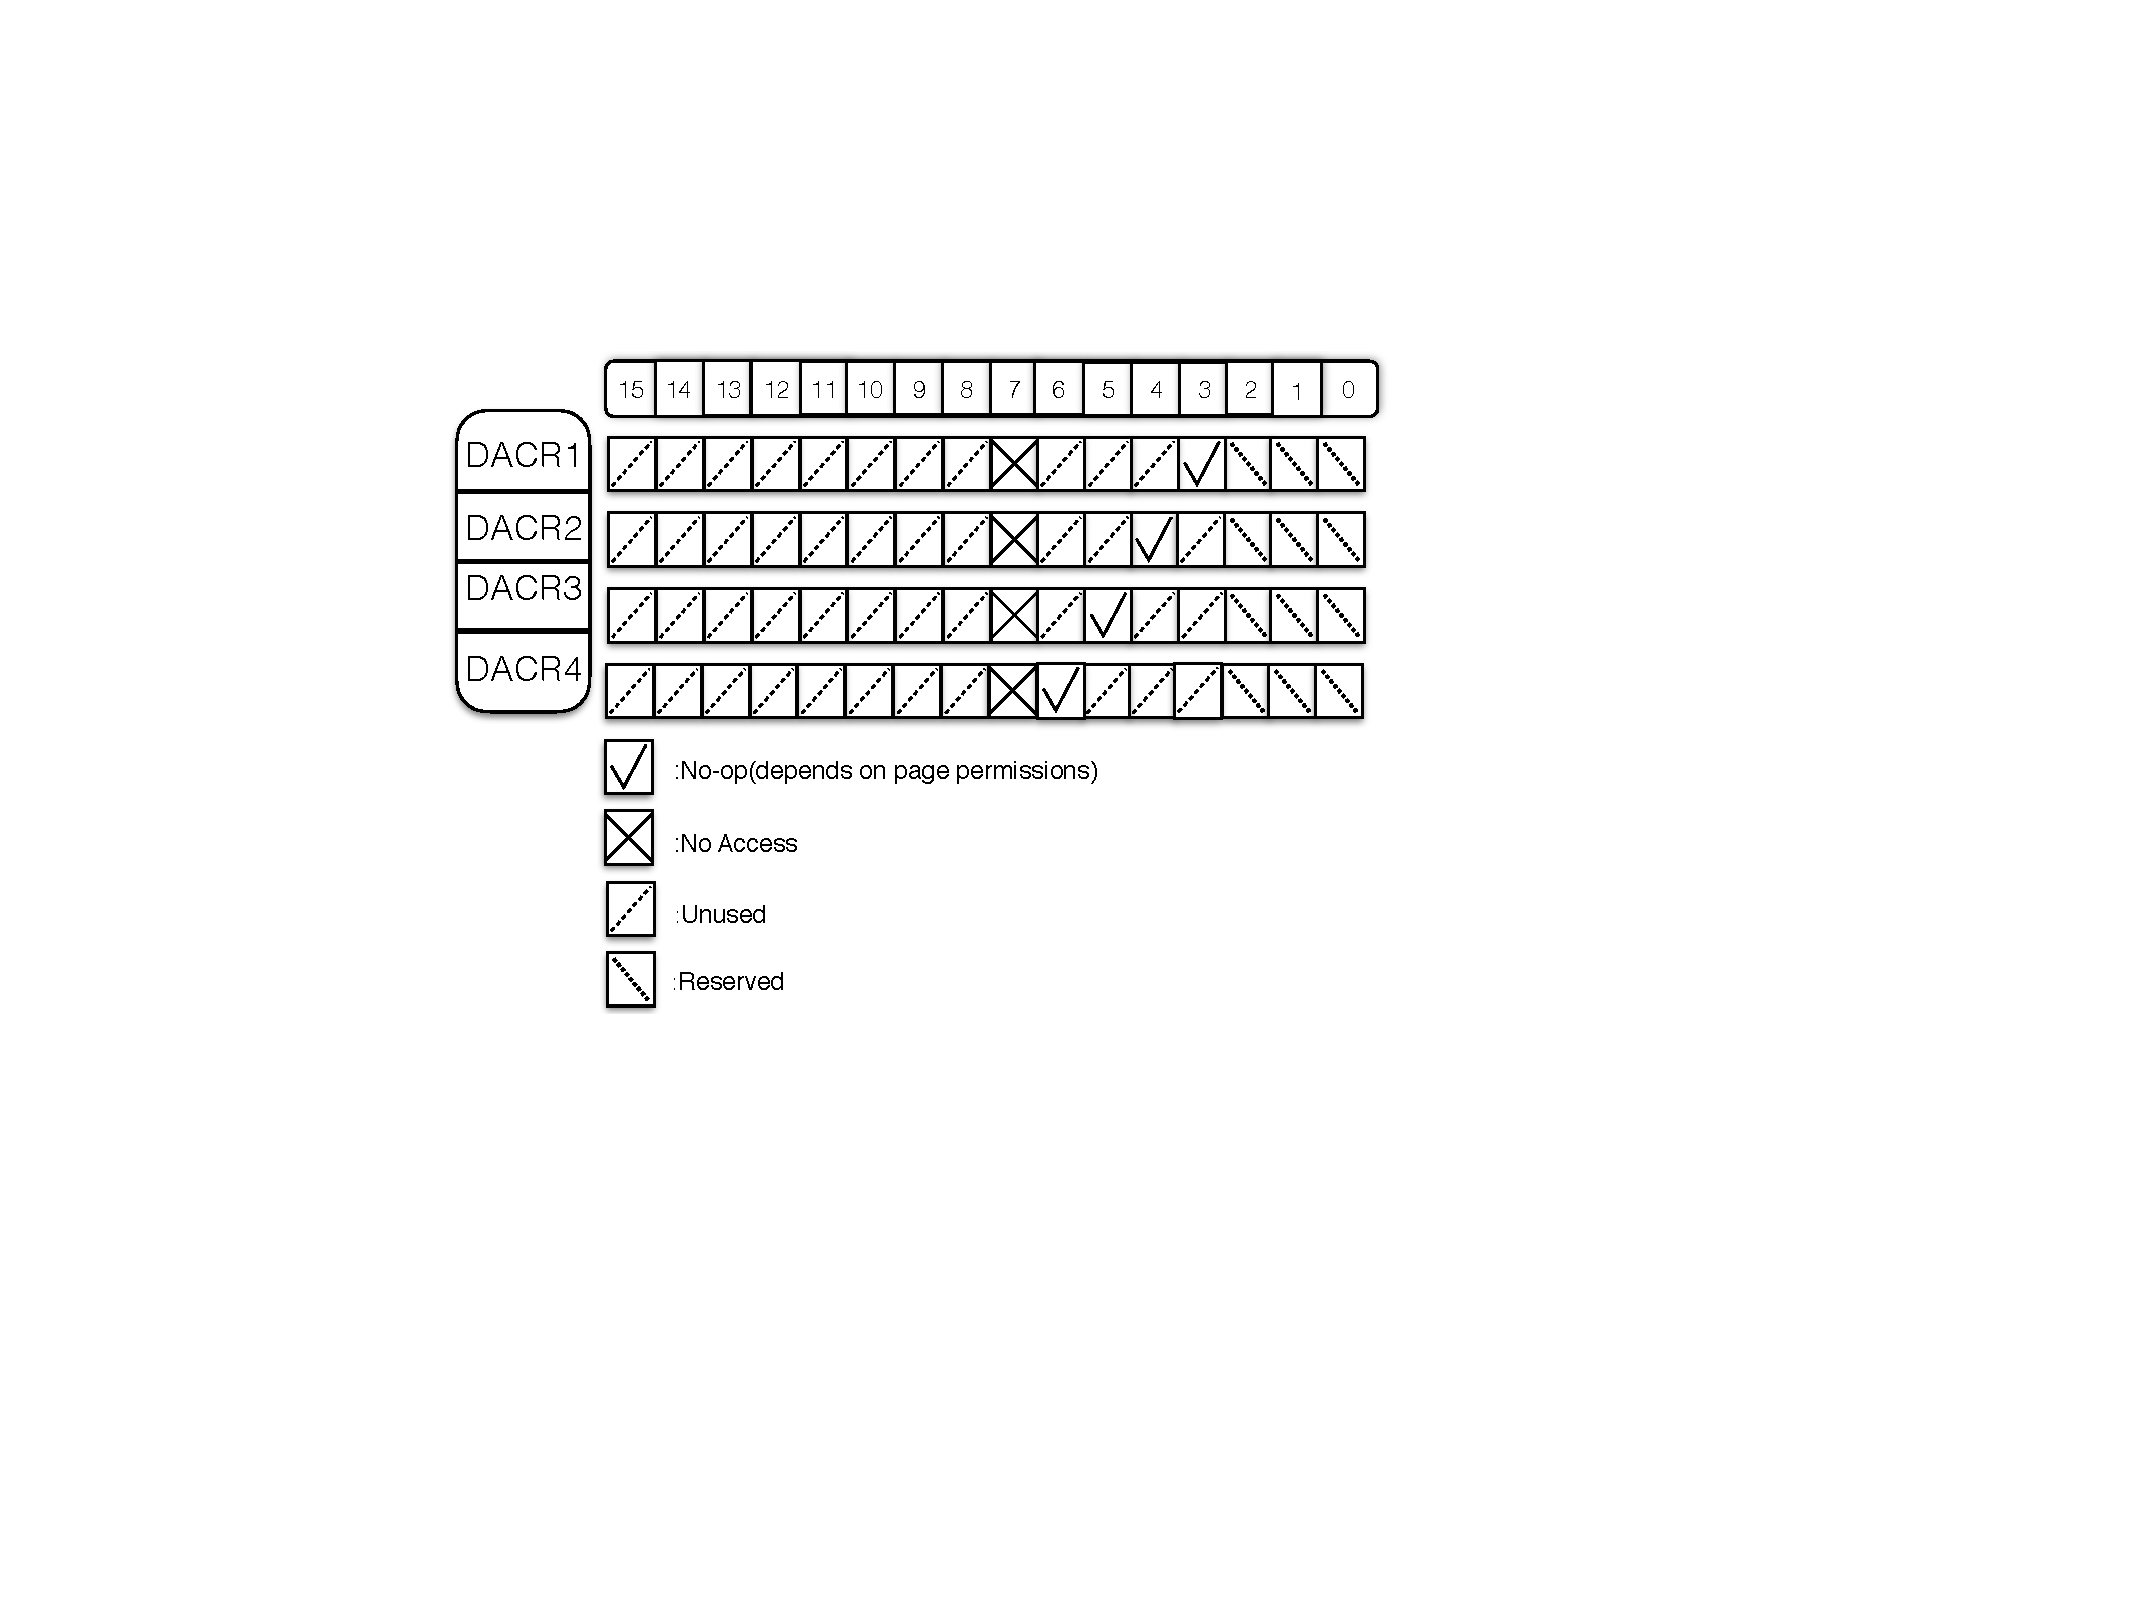
\includegraphics[width=\textwidth]{shreds/figures/dacr}
		\caption{The DACR setup for a quad-core system, where $k=4$. The first 3 domains ($Dom_{0}-Dom_{2}$) are reserved by Linux. Each core has a designated domain ($Dom_{3}-Dom_{6}$) that it may access when executing a shred. No CPU can access $Dom_{7}$. 
		 }
		\label{fig:dacr_setup}
	\end{minipage}
 \hfill
	\begin{minipage}[b]{0.4\textwidth}
		\centering	
		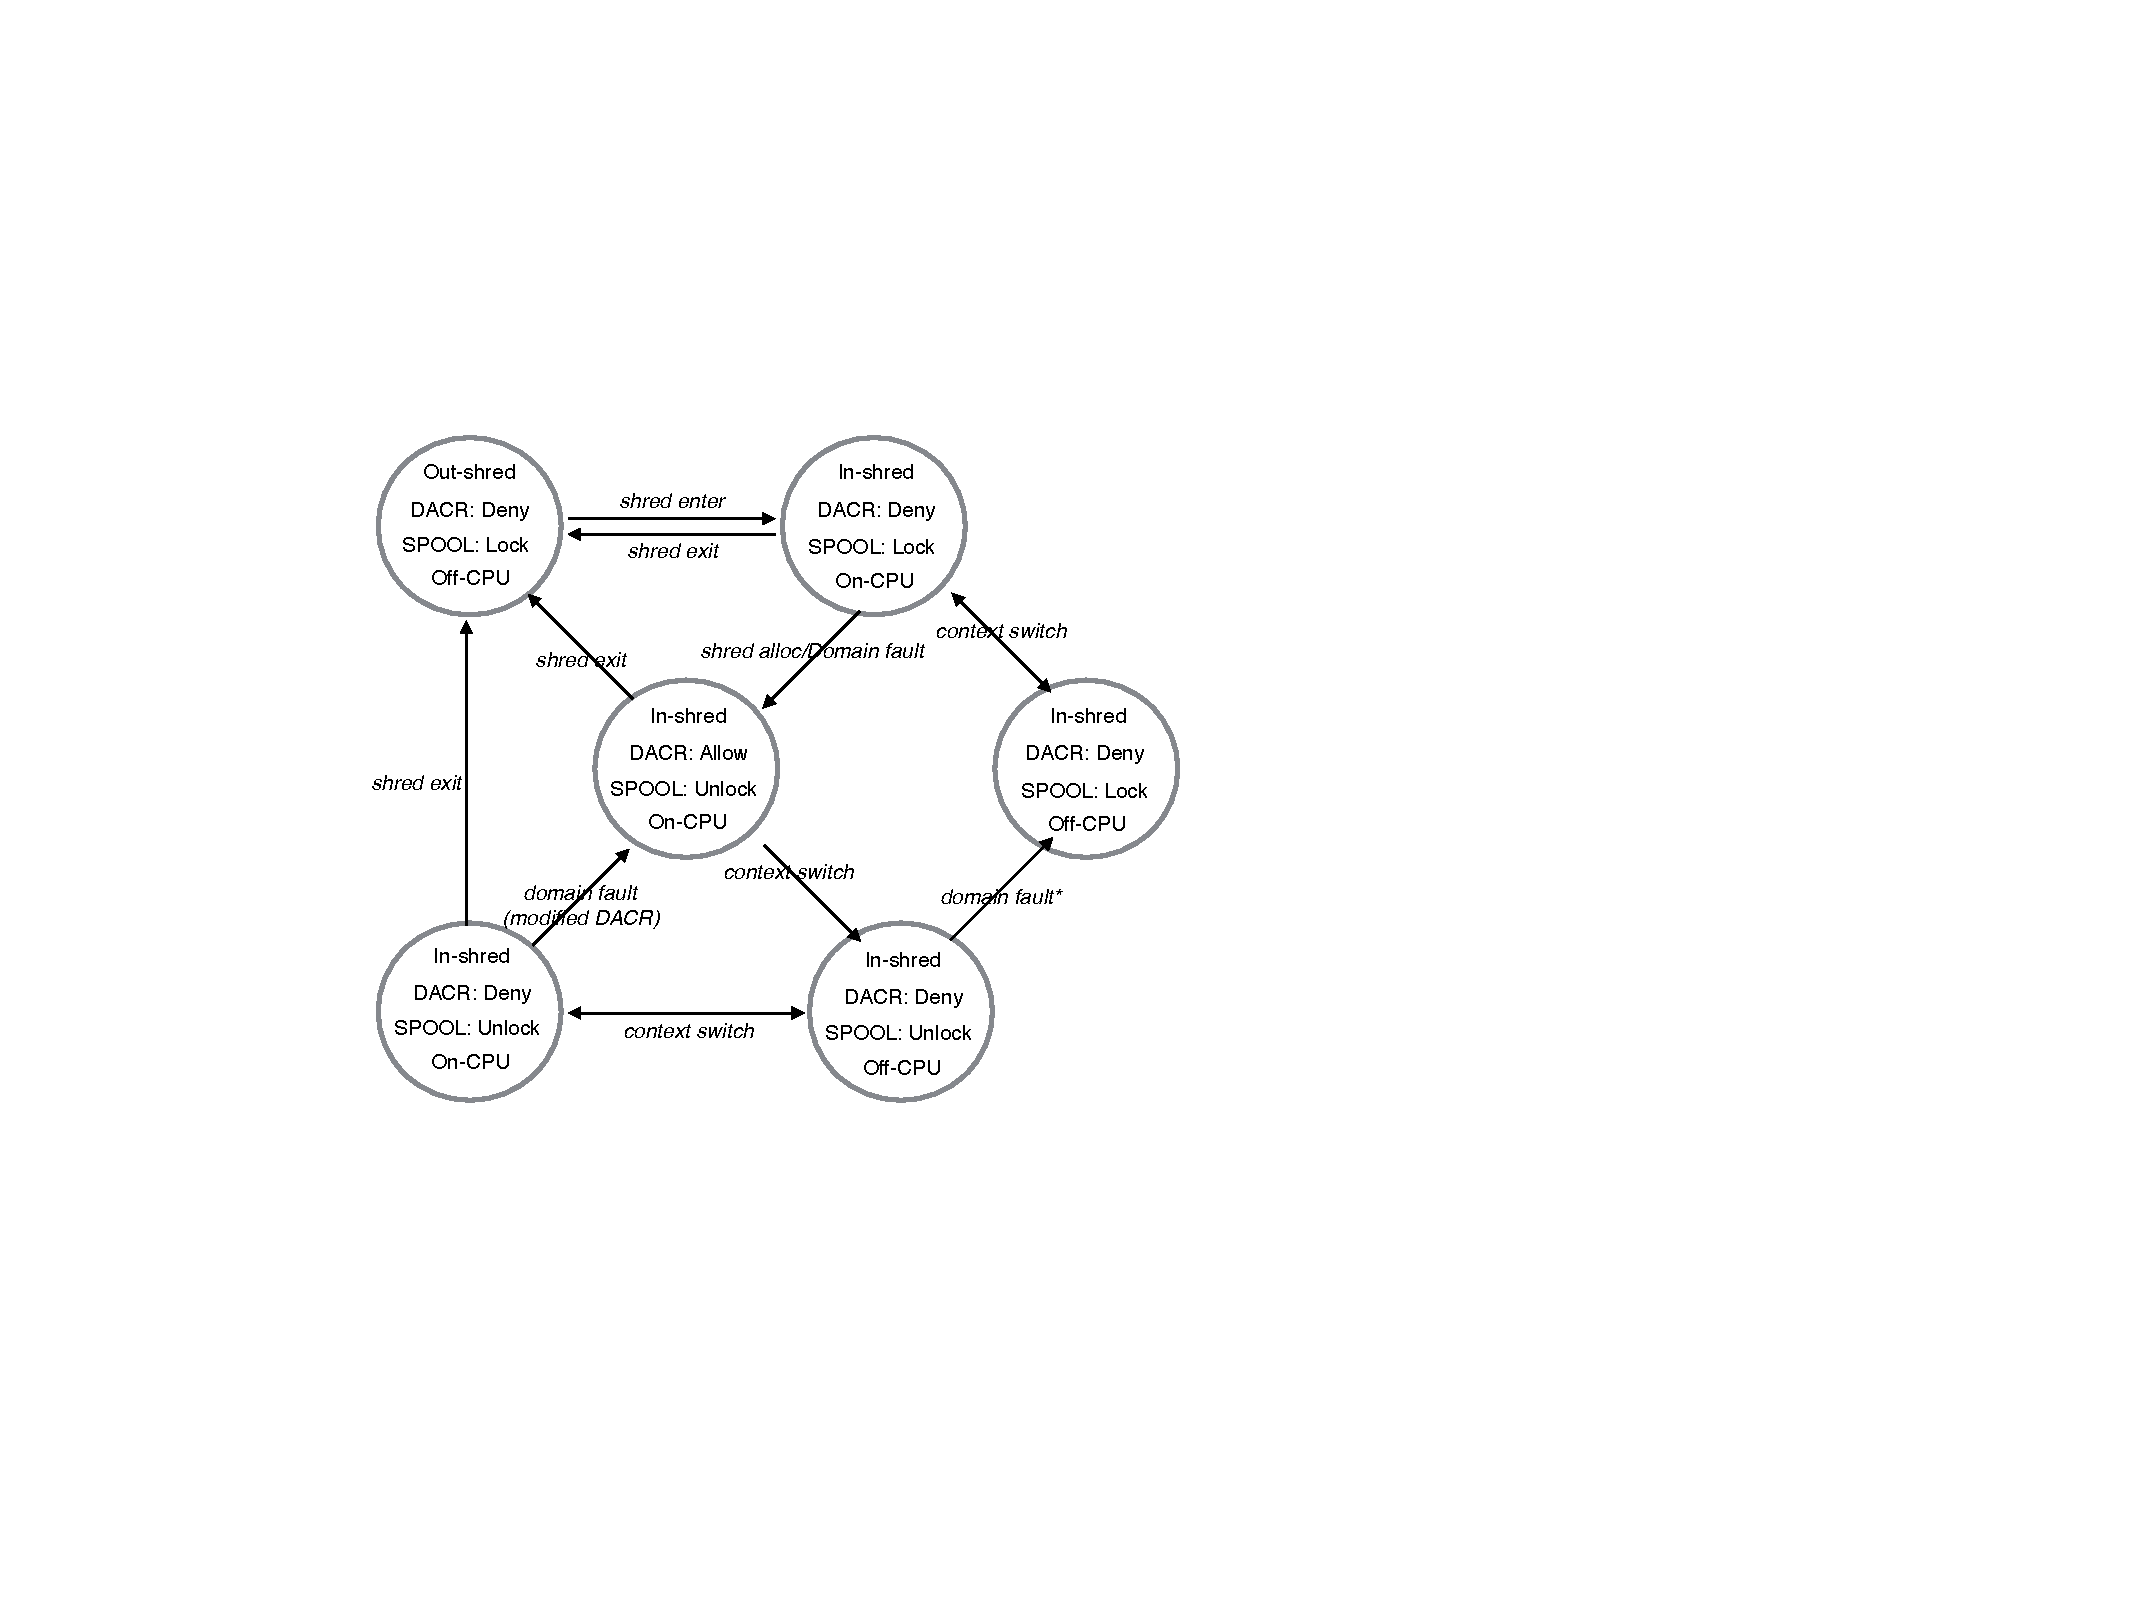
\includegraphics[width=\textwidth]{shreds/figures/shred_state_transition}
		\caption{A shred's transition of states}
		\label{fig:shredstat}
	\end{minipage}
\end{figure*}

S-driver uses the $k$ CPUs and the $k+1$ domains for executing shreds and protecting s-pools. 
When a shred starts or resumes its execution on $CPU_{i}$, S-driver assigns its associated s-pool to $Dom_{i}$, and therefore, the shred can freely access its s-pool while other concurrent threads, if any, cannot. 
When the shred terminates or is preempted, S-driver assigns its s-pool to $Dom_{k+1}$, which prevents any access to the pool from that moment on. 
As a result, S-driver allows or denies access to s-pools on a per-CPU basis, depending on if an associated shred occupies the CPU. 
Even if any malicious code manages to run concurrently alongside the shred inside the same process on another CPU, it cannot access the shred's s-pool without triggering domain faults. Thus, $P1$ is achieved. 

% performance and optimization 
It is reasonably efficient to switch s-pools to different domains upon shred entries and exits are. These operations do not involve heavy page table switches as process- or VM-based solutions do. They only require a shallow walk through of the first level page table and updates to the PDEs pointing to the s-pools in question. Besides, they do not trigger full TLB flushes as our design uses the per-address TLB eviction interface ({\tt flush\_tlb\_page}) and only invalidates the TLB entries related to the updated PDEs. 
To further reduce the overhead, we invent a technique called {\em lazy domain adjustment}: when a shred is leaving $CPU_{i}$, without adjusting any domain assignment, S-driver quickly changes the DACR to revoke the CPU's access to $Dom_{i}$ and lets the CPU's execution continue. It does not assign the s-pool used by the previous shred to $Dom_{k+1}$ until a domain fault happens (\ie another shred coming to the CPU and accessing its s-pool). The lazy domain adjustment avoids unnecessary domain changes and halves the already small overhead in some test cases.

%\begin{figure}[t]
%\begin{center}
%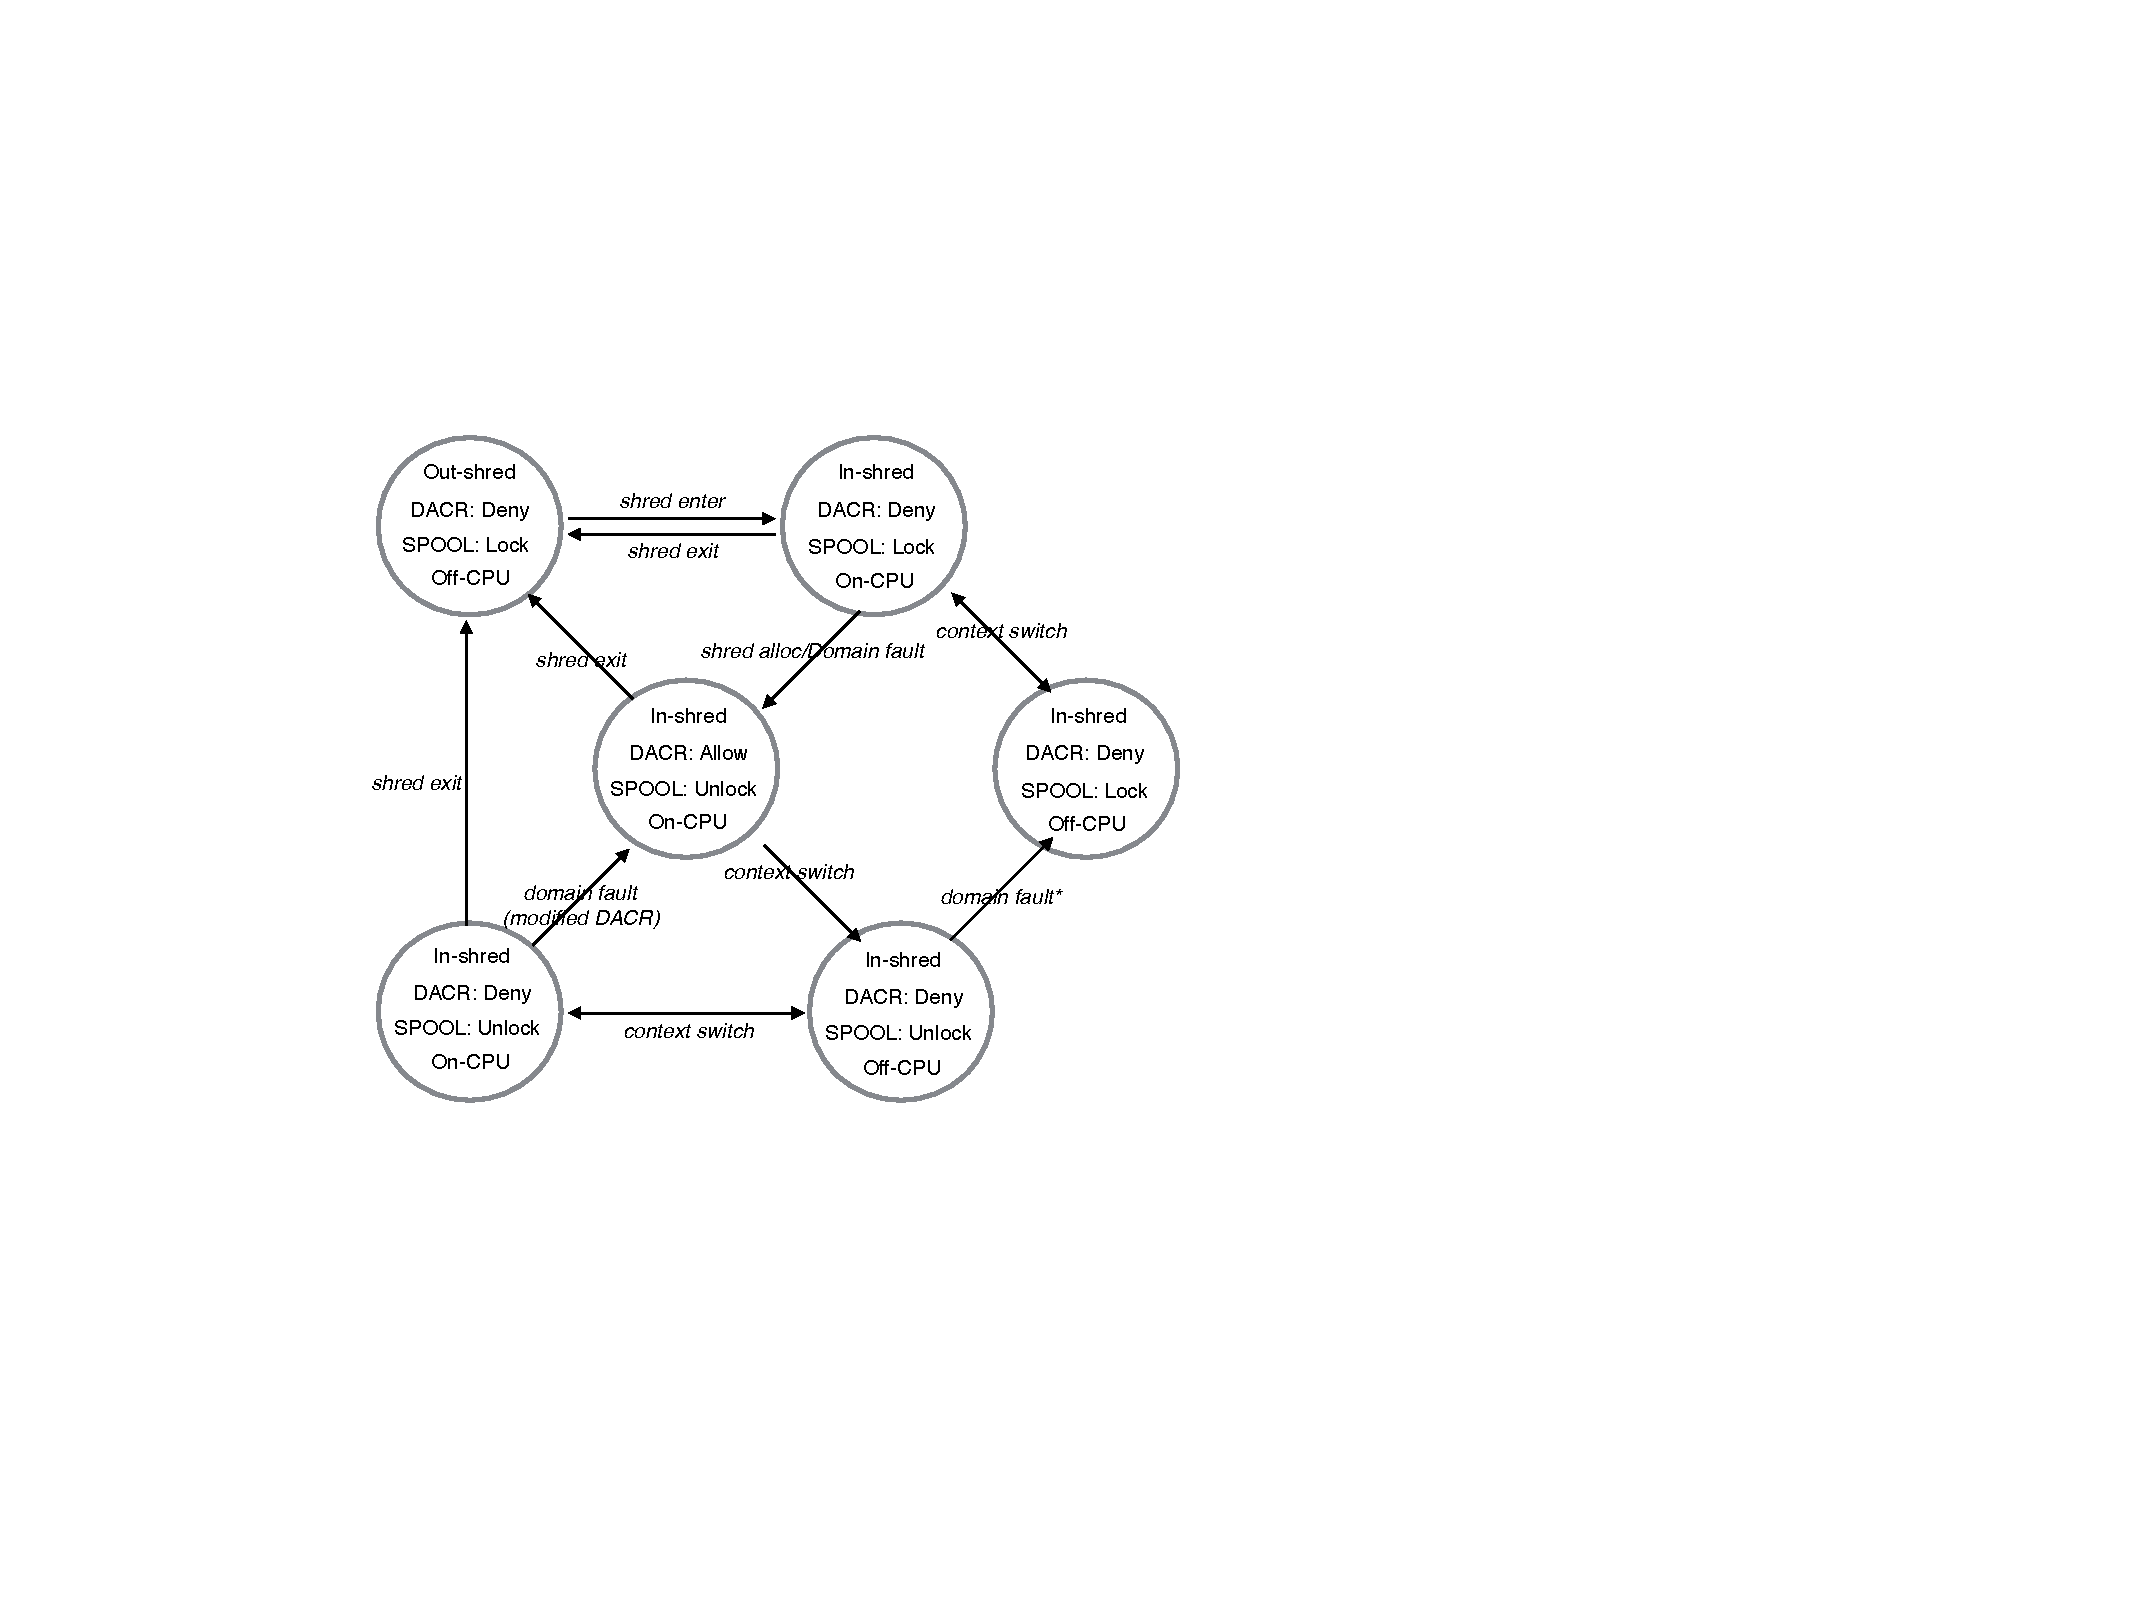
\includegraphics[scale=0.65]{shreds/figures/shred_state_transition}
%\caption{A shred's transition of states}
%\label{fig:shredstat}
%\end{center}
%\end{figure}

Figure~\ref{fig:shredstat} shows how S-driver orchestrates the transitions of a shred's states in response to the API calls, context switches, and domain faults. Each state is defined by a  combination of four properties:  

\begin{itemize}
\item $Shred$ = \{In-shred $|$ Out-shred\}: if the shred has started or exited. 
\item $DACR$ = \{Allow $|$ Deny\}: if the DACR allows or denies the current CPU to access its domain. 
\item $SPOOL$ = \{Lock $|$ Unlock\}: if the associated s-pool is locked or not. 
\item $CPU$ = \{On-CPU $|$ Off-CPU\}: if the shred is running on a CPU or not. 
\end{itemize}

The transition starts from the top, left circle, when the shred has not started and its s-pool is locked. After {\tt shred\_enter} is called, S-driver starts the shred, but it will not adjust the DACR or the s-pool access till a domain fault or a {\tt spool\_alloc} call due to the lazy domain adjustment in effect. When a context switch happens in the middle of the shred execution with unlocked DACR and s-pool, S-driver instantly sets the DACR to Deny but (safely) leaves the s-pool open. Later on, if a domain fault occurs, S-driver locks the previous s-pool because the fault means that the current code running on the CPU is in-shred and is trying to access its s-pool. If a domain fault never occurs till the shred regains the CPU, S-driver does not need to change any domain or s-pool settings, in which case the lazy domain adjustment saves two relatively heavy s-pool locking and unlocking operations. 
 
\point{Secure stacks for shreds}
%shadow stack support and switch 
Although S-compiler forbids unsanitized data flows from s-pools to unprotected memory regions, it has to allow in-shred code to copy s-pool data to local variables, which would be located in the regular stack and potentially accessible to in-process malicious code. 
To prevent secret leaks via stacks, S-driver creates a secure stack for each shred, allocated from its associated s-pool. When code execution enters a shred, S-driver transparently switches the stack without the application's knowledge: it copies the current stack frame to the secure stack and then overwrites the stack pointer. When the shred exits or encounters a signal to be handled outside of the shred, S-driver restores the regular stack.
As a result, local variables used by shreds never exist in regular stacks, and therefore cannot leak secrets.

\point{Runtime protection of shreds}
In addition to enabling and securing shreds and s-pools, S-driver also protects the inline reference monitor (IRM) that S-compiler plants in shred code. 
S-driver write-protects the memory pages containing the instrumented code and the associated data in memory.
It also pins the pages in s-pools in memory to prevent leaks via memory swap.  
Given that our threat model assumes the existence of in-process adversaries, S-driver also mediates the system calls that malicious code in user space may use to overwrite the page protection, dump physical memory via {\tt /dev/*mem}, disturb shreds via {\tt ptrace}, or load untrusted kernel modules. 
For each program using shreds, S-driver starts this mediation before loading the program code, avoiding pre-existing malicious code. 

S-driver's system call mediation also mitigates the attacks that steal secret data, not directly from s-pools, but from the I/O media where secret data are loaded or stored. 
For instance, instead of targeting the private key loaded in an s-pool, an in-process attacker may read the key file on disk. 
S-driver monitors file-open operations insides shreds. When the first time a file $F$ is accessed by a shred $S$, S-driver marks $F$ as a shred-private file and only allows shreds that share the same s-pool with $S$ to access $F$. This restriction is persistent and survives program and system reboots. 
As a result, an attacker can read $F$ only if she manages to intrude the program during its first run and access $F$ before a shred does. Although not completely preventing such attacks, S-driver makes them very difficult to succeed in reality. 
For a complete remedy, we envision a new primitive for in-shred code to encrypt and decrypt secret data with a persistent key assigned to each s-pool and automatically managed by S-driver. However, our current prototype does not support this primitive. 


It is worth noting that, although the system call mediation can prevent user-space malicious code that tries to break shreds via the system interfaces, it is a more intrusive and less configurable design choice than the well-known access control and capability frameworks, such as SELinux, AppArmor, and Capsicum~\cite{watson2010capsicum}. 
However, we leave the integration with those systems as future work because the system call mediation is easy to implement and is sufficient for the prototyping purpose. 



\subsection{Implementation}
\label{shreds:sec:impl}

We built S-compiler based on LLVM~\cite{lattner2004llvm} and its C front-end  Clang~\cite{clang}. We built S-driver with Linux as the reference OS. The implemented system was deployed and evaluated on a quad-core ARM Cortex-A7 computer (Raspberry Pi 2 Model B running Linux 4.1.15).

\point{S-compiler}
The modular and pass-based architecture of LLVM allows us to take advantage of the existing analyzers and easily extends the compilation pipeline. 
S-compiler adds two new passes to LLVM: the shred analysis pass and the security instrumentation pass. Both operate on LLVM bitcode as the IR. 

The analysis pass carries out the checks on the usages and security properties of shreds, as described in \S~\ref{shreds:sec:design}. 
We did not use LLVM's built-in data flow analysis for those checks due to its overly heuristic point-to analysis and the unnecessarily conservative transfer functions.
Instead, we implemented our specialized data flow analysis based on the basic round-robin iterative algorithm, with weak context sensitivity and a straightforward propagation model (i.e., only tracking value-conserving propagators).
We also had to extend LLVM's compilation pipeline because it by default only supports intra-module passes while S-compiler needs to perform inter-module analysis. We employed a linker plugin, called the Link-Time Optimization (LTO), to cross link the IR of all compilation modules and feed the linked IR to our analyzers. 


The instrumentation pass uses the LLVM IR Builder interfaces to insert security checks into the analyzed IR, which are necessary for enforcing the in-shred control flow regulations and preventing dynamic data leaks. 

\IncMargin{1em}
\begin{algorithm}
\small
\SetKwData{Spool}{s\_pool}
\SetKwData{Owner}{s\_owner}
\SetKwData{FaultThread}{fault\_thread}
\SetKwData{CPUDomain}{cpu\_domain}
\SetKwData{SpoolDomain}{s\_pool\_domain}
\SetKwFunction{FindSpool}{FindSpool}
\SetKwFunction{GetOwner}{GetOwner}
\SetKwFunction{GetCPUDomain}{GetCPUDomain}
\SetKwFunction{GetSpoolDomain}{GetSpoolDomain}
\SetKwFunction{BadArea}{bad\_area}
\SetKwFunction{GoodArea}{good\_area}
\SetKwFunction{RestoreDACR}{RestoreDACR}
\SetKwFunction{UnlockSPool}{UnlockSPool}
\SetKwFunction{AdjustSPool}{AdjustSPool}
\SetKwFunction{LockActiveSPoolList}{LockOtherActiveSPools}
\SetKwInOut{Input}{input}
\SetKwInOut{Output}{result}
\Input{The faulting virtual address $fault\_addr$}
\Output{Recover from the domain fault, or kill the faulting thread}
\BlankLine
\emph{/*Identity check*/}\\
  \Spool$\leftarrow$ \FindSpool{$fault\_addr$}\;
  \Owner$\leftarrow$ \GetOwner{$\Spool$}\;
  \If{\FaultThread is NOT in shred}{goto \BadArea}
  \If{\FaultThread is NOT \Owner}{goto \BadArea}
\BlankLine
\emph{/*Recover from domain fault*/}\\
  \CPUDomain$\leftarrow$ \GetCPUDomain{}\;
  \SpoolDomain$\leftarrow$ \GetSpoolDomain{\Spool}\;
   \If{\Spool is unlocked}
   {
   		  
          \If{\CPUDomain $=$ \SpoolDomain}
          {
            \emph{/*No need to change domain for s\_pool*/} \\
            \RestoreDACR{}\;
          }
          \Else
   		  {
   		    \AdjustSPool{\CPUDomain}  
   		  }
   }
    \Else
    {
    	\UnlockSPool{\CPUDomain} 
    }
   \LockActiveSPoolList{\Spool}\;
\caption{Domain Fault Handler}\label{dom_fault_handler}
\end{algorithm}
\DecMargin{1em}

\point{S-driver}
We built S-driver into a Loadable Kernel Module (LKM) for Linux. 
S-driver creates a virtual device file ({\tt /dev/shreds}) to handle the {\tt ioctl} requests made internally by the shred APIs. 
It uses 13 out of 16 memory domains to protect s-pools because the recent versions of Linux kernel for ARM already occupies 3 domains (for isolating device, kernel, and user-space memory). 
S-driver uses the available domains to protect unlimited s-pools and controls each CPU's access to the domains as described in \S~\ref{shreds:sec:design}.
Since Linux does not provide callback interfaces for drivers to react to scheduling events, in order to safely handle context switches or signal dispatches in shreds, 
S-driver dynamically patches the OS scheduler so that, during every context switch, the DACR of the current CPU is reset, which locks the open s-pool, if any. 
The overhead of this operation is negligible because resetting the DACR only takes a single lightweight instruction. 
To capture illegal access to s-pools and lazily adjust domain assignments, 
S-driver registers itself to be the only handler of domain faults and is triggered whenever a domain violation happens. 
Algorithm~\ref{dom_fault_handler} shows how S-driver handles a domain fault. 
Purely implementing S-driver as a LKM allows shreds to be introduced into a host without installing a custom-build kernel image.


\subsection{Analysis}
\label{rpo:sec:analysis}

% \begin{table}[t]
    \caption{Narrowing down the Common Crawl to the candidate set used in our analysis (from left to right).}
    \label{rpo:tab:dataset_stats}
    \centering
    \footnotesize
    \begin{tabular}{lrrr}
    \toprule
    \multicolumn{2}{r}{\textbf{Relative CSS}} & \textbf{Alexa Top 1M} & \textbf{Candidate Set} \\
    \midrule
    All Pages & 203,609,675 & 141,384,967 & 136,793,450 \\
    Tested Pages & 53,725,270 & 31,448,446 & 30,991,702 \\
    Sites & 5,960,505 & 223,212 & 222,443 \\
    Document Types & 9,833 & 2,965 & 2,898 \\
    \bottomrule
    \end{tabular}
\end{table}


For the purposes of our analysis, we gradually narrow down the seed data from
the Common Crawl to pages using relative style paths in the Alexa Top 1\,M,
reflecting injected style directives under RPO, and being exploitable due to
quirks mode rendering.

% Table~\ref{rpo:tab:dataset_stats} shows a summary of our dataset. \textit{Tested
% Pages} refers to the set of randomly selected pages from the page groups as
% discussed in Section~\ref{rpo:sec:methodology:candidate}. For brevity,
% we are referring to \textit{Tested Pages} wherever we mention pages in the
% remainder of the paper.

\subsubsection{Relative Stylesheet Paths}
\label{rpo:sec:analysis:relative}

\begin{figure}[t]
\centering
\begin{minipage}{.32\textwidth}
    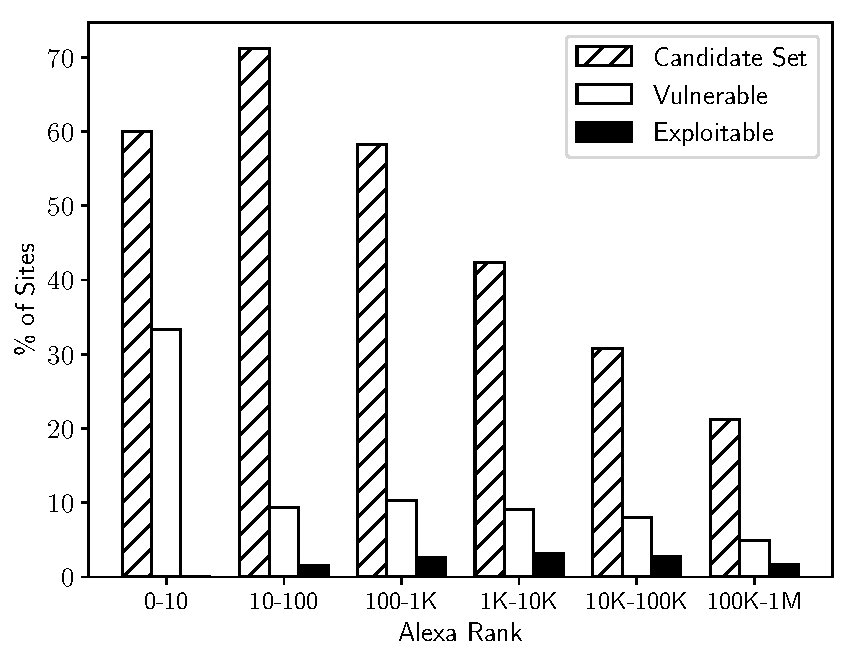
\includegraphics[width=1\textwidth,height=.8\textwidth]{rpo/figures/alexa_rank}
    \caption{Percentage of the Alexa site ranking in our candidate set
             (exponentially increasing bucket size).}
    \label{rpo:fig:analysis:alexa_rank}
\end{minipage}
\hfill
\begin{minipage}{.32\textwidth}
    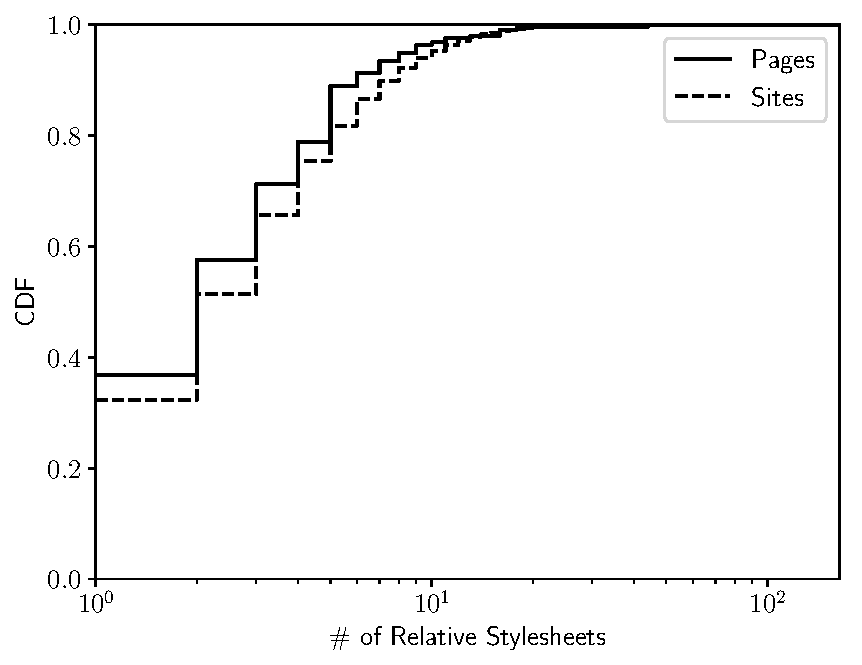
\includegraphics[width=1\textwidth,height=.8\textwidth]{rpo/figures/relative_stylesheets}
    \caption{CDF of total and maximum number of relative stylesheets per web
             page and site, respectively.}
    \label{rpo:fig:analysis:relative_stylesheets}
\end{minipage}
\hfill
\begin{minipage}{.32\textwidth}
    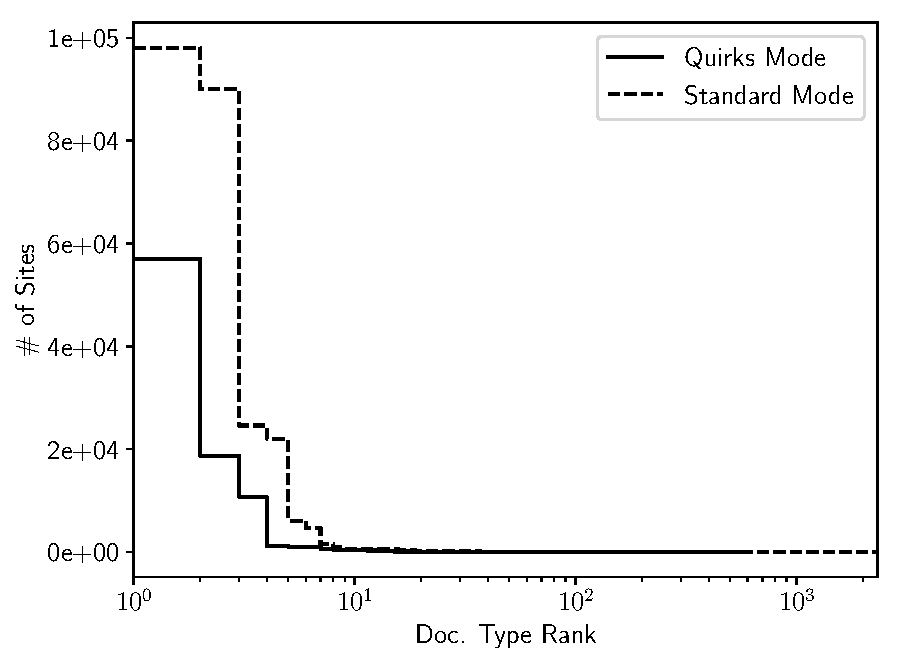
\includegraphics[width=1\textwidth,height=.8\textwidth]{rpo/figures/doctypes_rank_sites}
    \caption{Number of sites containing at least one page with a certain
             document type (ordered by doctype rank).}
    \label{rpo:fig:analysis:doctypes_rank_sites}
\end{minipage}
\end{figure}


To assess the extent to which our Common Crawl-seeded candidate set covers sites
of different popularity, consider the hatched bars in
Figure~\ref{rpo:fig:analysis:alexa_rank}. Six out of the ten largest sites
according to Alexa are represented in our candidate set. That is, they are
contained in the Common Crawl, and have relative style paths. The figure shows
that our candidate set contains a higher fraction of the largest sites and a
lower fraction of the smaller sites. Consequently, our results better represent
the most popular sites, which receive most visitors, and most potential victims
of RPO attacks.

While all the pages in the candidate set contain at least one relative
stylesheet path, Figure~\ref{rpo:fig:analysis:relative_stylesheets} shows that
63.1\,\% of them contain multiple relative paths, which increases the chances of
finding a successful RPO and style injection point.

\subsubsection{Vulnerable Pages}
\label{rpo:sec:analysis:vulnerable}

\begin{table*}[t]
    \centering
    \caption{Vulnerable/exploitable pages and sites in the candidate set (IE using framing).}
    \label{rpo:tab:vulnerable_exploitable_result}
    \footnotesize
    \begin{tabular}{lrrrrrr}
    \toprule
    \multirow{2}{*}{\textbf{Technique}} &
    \multicolumn{2}{c}{\textbf{Vulnerable}} &
    \multicolumn{2}{c}{\textbf{Exploitable (Chrome)}} &
    \multicolumn{2}{c}{\textbf{Exploitable (IE)}} \\

    \cmidrule[0.5pt](lr){2-3}
    \cmidrule[0.5pt](lr){4-5}
    \cmidrule[0.5pt](lr){6-7}

    &
    \textbf{Pages} &
    \textbf{Sites} &
    \textbf{Pages} &
    \textbf{Sites} &
    \textbf{Pages} &
    \textbf{Sites}
    \\

    \midrule

    Path Parameter & 309,079 (1.0\%) & 9,136 (4.1\%) & 6,048 (\textless 0.1\%) & 1,025 (0.5\%) & 52,344 (0.2\%) & 3,433 (1.5\%) \\
    Encoded Path & 53,502 (0.2\%) & 1,802 (0.8\%) & 3 (\textless 0.1\%) & 2 (\textless 0.1\%) & 24 (\textless 0.1\%) & 5 (\textless 0.1\%) \\
    Encoded Query & 89,757 (0.3\%) & 1,303 (0.6\%) & 23 (\textless 0.1\%) & 20 (\textless 0.1\%) & 137 (\textless 0.1\%) & 43 (\textless 0.1\%) \\
    Cookie & 15,656 (\textless 0.1\%) & 1,030 (0.5\%) & 4,722 (\textless 0.1\%) & 81 (\textless 0.1\%) & 2,447 (\textless 0.1\%) & 238 (0.1\%) \\

    \midrule

    Total & 377,043 (1.2\%) & 11,986 (5.4\%) & 10,781 (<0.1\%) & 1,106 (0.5\%) & 54,853 (0.2\%) & 3,645 (1.6\%) \\

    \bottomrule
    \end{tabular}

\end{table*}


We consider a candidate page vulnerable if one of the style injection techniques
of Section~\ref{rpo:sec:methodology:vulnerable} succeeds. In other
words, the server's response should reflect the injected payload. Furthermore,
we conservatively require that the response not contain a \texttt{base} tag
since a correctly configured base tag can prevent path confusion.

Table~\ref{rpo:tab:vulnerable_exploitable_result} shows that 1.2\,\% of pages
are vulnerable to at least one of the injection techniques, and 5.4\,\% of sites
contain at least one vulnerable page. The path parameter technique is most
effective against pages, followed by the encoded query and the encoded path
techniques. Sites that are ranked higher according to Alexa are more likely to
be vulnerable, as shown in Figure~\ref{rpo:fig:analysis:alexa_rank}, where
vulnerable and exploitable sites are relative to the candidate set in each
bucket. While one third of the candidate set in the Top~10 (two out of six
sites) is vulnerable, the percentage oscillates between 8 and 10\,\% among the
Top~100\,k. The candidate set is dominated by the smaller sites in the ranks
between 100\,k and 1\,M, which have a vulnerability rate of 4.9\,\% and push
down the average over the entire ranking.

% A \texttt{base} tag in the server response can prevent path confusion because it
% indicates how the browser should expand relative paths. We observed a number of
% inconsistencies with respect to its use. At first, 603 pages on 60 sites
% contained a \texttt{base} tag in their response; however, the server response
% after injecting our payload did not contain the tag anymore, rendering these
% pages potentially exploitable. Furthermore, Internet Explorer's implementation
% of the \texttt{base} tag appears to be broken. When such a tag is present,
% Internet Explorer fetches two URLs for stylesheets---one expanded according to
% the base URL specified in the tag, and one expanded in the regular, potentially
% ``confused'' way of using the page URL as the base. In our experiments, Internet
% Explorer always applied the ``confused'' stylesheet, even when the one based on
% the \texttt{base} tag URL loaded faster. Consequently, \texttt{base} tags do not
% appear to be an effective defense against RPO in Internet Explorer (They seem to
% work as expected in other browsers, including Edge).


\subsubsection{Exploitable Pages}
\label{rpo:sec:analysis:exploitable}

To test whether a vulnerable page was exploitable, we opened it in Chrome,
injected a style payload with an image reference (randomly generated URL), and
checked if the image was indeed loaded. This test succeeded for 2.9\,\% of
vulnerable pages; 0.5\,\% of sites in the candidate set had at least one
exploitable page (Table~\ref{rpo:tab:vulnerable_exploitable_result}).

% In the following, we explore various factors that may impact whether a
% vulnerable page can be exploited, and we show how some of these partial defenses
% can be bypassed.

% \paragraph{Document Types}
% \label{rpo:sec:analysis:doctypes}

% \begin{table}[t]
\centering
\begin{minipage}[t]{.55\textwidth}
    \caption{Summary of document type usage in sites.\newline}
    \label{rpo:tab:doctypes_summary}
    \centering
    \footnotesize
    \begin{tabular}{lrr}
    \toprule
    \textbf{Doc. Type} & \textbf{At Least One Page} & \textbf{All Pages} \\
    \midrule

    None & 56,985 (25.6\%) & 19,968 (9.0\%) \\
    Quirks & 27,794 (12.5\%) & 7,720 (3.5\%) \\
    None or Quirks & 71,597 (32.2\%) & 30,040 (13.5\%) \\
    \addlinespace
    Standards & 192,403 (86.5\%) & 150,846 (67.8\%) \\    
    \bottomrule
    \end{tabular}
\end{minipage}
\hfill
\begin{minipage}[t]{.43\textwidth}
    \caption{Quirks mode document types by browser.}
    \label{rpo:tab:doctypes_browsers}
    \centering
    \footnotesize
    \begin{tabular}{llr}
    \toprule

    \textbf{Browser} &
    \textbf{OS} &
    \textbf{Doc. Types} \\

    \midrule
    Chrome 55 & Linux & 1,378 (31.9\,\%) \\
    Opera 42 & Linux & 1,378 (31.9\,\%) \\
    Safari 10 & macOS & 1,378 (31.9\,\%) \\
    \addlinespace
    Firefox 50 & Linux & 1,326 (30.7\,\%) \\
    \addlinespace
    Edge 38 & Windows & 1,319 (30.5\,\%) \\
    IE 11 & Windows & 1,319 (30.5\,\%) \\
    \bottomrule
    \end{tabular}
\end{minipage}
\end{table}


% \begin{table}[t]
    \caption{Most frequent document types causing all browsers to render
    in quirks mode, as well as the sites that use at least one such
    document type.}
    \label{rpo:tab:top_quirksmode_doctypes}
    \centering
    \footnotesize
    \begin{tabular}{lrr}
    \toprule
    \textbf{Document Type (shortened)} & \textbf{Pages} & \textbf{Sites} \\
    \midrule
    (none) & 1,818,595 (5.9\,\%) & 56,985 (25.6\,\%) \\
    "-//W3C//DTD HTML 4.01 Transitional//EN" & 721,884 (2.3\,\%) & 18,648 (8.4\,\%) \\
    "-//W3C//DTD HTML 4.0 Transitional//EN" & 385,656 (1.2\,\%) & 11,566 (5.2\,\%) \\
    "-//W3C//DTD HTML 3.2 Final//EN" & 22,019 (<0.1\,\%) & 1,175 (0.5\,\%) \\
    "-//W3C//DTD HTML 3.2//EN" & 10,839 (<0.1\,\%) & 927 (0.4\,\%) \\
    \midrule
    All & 3,046,449 (9.6\,\%) & 71,597 (32.2\,\%) \\
    \bottomrule
    \end{tabular}
\end{table}


% HTML document types play a significant role in RPO-based style injection attacks
% because browsers typically parse resources with a non-CSS content type in a CSS
% context only when the page specifies an ancient or non-standard HTML document
% type (or none at all). The pages in our candidate set contain a total of 4,318
% distinct document types. However, the majority of these unique document types
% are not standardized and differ from the standardized ones only by small
% variations, such as forgotten spaces or misspellings.

% To determine how browsers interpret these document types (i.e., whether they
% cause them to render a page in standards or quirks mode), we designed a
% controlled experiment. For each unique document type, we set up a local page
% with a relative stylesheet path and carried out an RPO attack to inject CSS
% using a payload similar to what we described in
% Section~\ref{rpo:sec:methodology:vulnerable}. We automatically opened
% the local page in Chrome, Firefox, Edge, Internet Explorer, Safari, and Opera,
% and we kept track of which document type caused the injected CSS to be parsed
% and the injected background image to be downloaded.

% Table~\ref{rpo:tab:doctypes_browsers} contains the results of this experiment.
% Even though the exact numbers vary among browsers, roughly a third of the unique
% document types we encountered result in quirks mode rendering. Not surprisingly,
% both Microsoft products Edge and Internet Explorer exhibit identical results,
% whereas the common Webkit ancestry of Chrome, Opera, and Safari also show
% identical results. Overall, 1,271 (29.4\,\%) of the unique document types force
% all the browsers into quirks mode, whereas 1,378 (31.9\,\%) of them cause at
% least one browser to use quirks mode rendering.
% Table~\ref{rpo:tab:top_quirksmode_doctypes} shows the most frequently used
% document types that force all the browsers into quirks mode, which includes the
% absence of a document type declaration in the page.

% To test how often Internet Explorer allows a page's document type to be
% overridden when loading it in an \texttt{iframe}, we created another controlled
% experiment using a local attack page framing the victim page, as outlined in
% Section~\ref{rpo:sec:methodology:exploitable}. Using Internet
% Explorer~11, we loaded our local attack page for each unique document type
% inside the frame, and tested if the injected CSS was parsed. While Internet
% Explorer parsed the injected CSS for 1,319 (30.5\,\%) of the document types in
% the default setting, the frame override trick caused CSS parsing for 4,248
% (98.4\,\%) of the unique document types.

% While over one thousand document types result in quirks mode, and around three
% thousand document types cause standards mode parsing, the number of document
% types that have been standardized is several orders of magnitude smaller. In
% fact, only a few (standardized) document types are used frequently in pages,
% whereas the majority of unique document types are used very rarely.
% Figure~\ref{rpo:fig:analysis:doctypes_rank_sites} shows that only about ten
% standards and quirks mode document types are widely used in pages and sites.
% Furthermore, only about 9.6\,\% of pages in the candidate set use a quirks mode
% document type; on the remaining pages, potential RPO style injection
% vulnerabilities cannot be exploited because the CSS would not be parsed (unless
% Internet Explorer is used). However, when grouping pages in the candidate set by
% site, 32.2\,\% of sites contain at least one page rendered in quirks mode
% (Table~\ref{rpo:tab:doctypes_summary}), which is one of the preconditions for
% successful RPO.

% \paragraph{Internet Explorer Framing}

% We showed above that by loading a page in a frame, Internet Explorer can be
% forced to disregard a standards mode document type that would prevent
% interpretation of injected style. To find out how often this technique can be
% applied for successful RPO attacks, we replicated our Chrome experiment in
% Internet Explorer, this time loading each vulnerable page inside a frame. Around
% 14.5\,\% of vulnerable pages were exploitable in Internet Explorer, five times
% more than in Chrome (1.6\,\% of the sites in the candidate set).

% Figure~\ref{rpo:fig:analysis:alexa_rank} shows the combined exploitability
% results for Chrome and Internet Explorer according to the rank of the site.
% While our methodology did not find any exploitable vulnerability on the six
% highest-ranked sites in the candidate set, between 1.6\,\% and 3.2\,\% of
% candidate sites in each remaining bucket were found to be exploitable. The
% highest exploitability rate occurred in the ranks 1\,k through 10\,k.

% Broken down by injection technique, the framing trick in Internet Explorer
% results in more exploitable pages for each technique except for cookie injection
% (Table~\ref{rpo:tab:vulnerable_exploitable_result}). One possible explanation
% for this difference is that the Internet Explorer crawl was conducted one month
% after the Chrome crawl, and sites may have changed in the meantime. Furthermore,
% we observed two additional impediments to successful exploitation in Internet
% Explorer that do not apply to Chrome. The framing technique is susceptible to
% frame-busting methods employed by the framed pages, and Internet Explorer
% implements an anti-MIME-sniffing header that Chrome appears to ignore. We
% analyze these issues below.

% \paragraph{Anti-Framing Techniques}

% Some sites use a range of techniques to prevent other pages from loading them in
% a frame~\cite{w2sp2010frame_busting}. One of these techniques is the
% \texttt{X-Frame-Options} header. It accepts three different values:
% \texttt{DENY}, \texttt{SAMEORIGIN}, and \texttt{ALLOW-FROM} followed by a
% whitelist of URLs.

% In the vulnerable dataset, 4,999 pages across 391 sites use this header
% correctly and as a result prevent the attack. However, 1,900 pages across 34
% sites provide incorrect values for this header, and we successfully attack 552
% pages on 2 sites with Internet Explorer.

% A related technique is the \texttt{frame-ancestors} directive provided by
% Content Security Policy. It defines a (potentially empty) whitelist of URLs
% allowed to load the current page in a frame, similar to \texttt{ALLOW-FROM}.
% However, it is not supported by Internet Explorer, thus it cannot be used to
% prevent the attack.

% Furthermore, developers may use JavaScript code to prevent framing of a page.
% Yet, techniques exist to bypass this
% protection~\cite{owasp_clickjacking_defence}. In addition, the attacker can use
% the HTML 5 \texttt{sandbox} attribute in the \texttt{iframe} tag and omit the
% \texttt{allow-top-navigation} directive to render JavaScript frame-busting code
% ineffective. However, we did not implement any of these techniques to allow
% framing, which means that more vulnerable pages could likely be exploited in
% practice.

% \paragraph{MIME Sniffing}

% A consequence of self-reference in the type of RPO studied in this paper is that
% the HTTP content type of the fake ``stylesheet'' is \texttt{text/html} rather
% than the expected \texttt{text/css}. Because many sites contain misconfigured
% content types, many browsers attempt to infer the type based on the request
% context or file extension (\textit{MIME sniffing}), especially in quirks mode.
% In order to ask the browser to disable content sniffing and refuse interpreting
% data with an unexpected or wrong type, sites can set the header
% \texttt{X-Content-Type-Options: nosniff}~\cite{sp2009contentsniff,firefox_mime_sniff,content_type_options}.

% To determine whether the injected CSS is still being parsed and executed in
% presence of this header while the browser renders in quirks mode, we ran an
% experiment similar to Section~\ref{rpo:sec:analysis:doctypes}. For each browser
% in Table~\ref{rpo:tab:doctypes_browsers}, we extracted the document types in
% which the browser renders in quirks mode, and for each of them, we set up a
% local page with a relative stylesheet path. We then opened the page in the
% browser, launched an RPO attack, and monitored if the injected CSS was executed.

% Only Firefox, Internet Explorer, and Edge respected this header and did not
% interpret injected CSS in any of the quirks mode document types. The remaining
% browsers did not block the stylesheet even though the content type was not
% \texttt{text/css}. With an additional experiment, we confirmed that Internet
% Explorer blocked our injected CSS payload when \texttt{nosniff} was set, even in
% the case of the framing technique.

% Out of all the vulnerable pages, 96,618 pages across 232 sites had a
% \texttt{nosniff} response header; 23 pages across 10 sites were confirmed
% exploitable in Chrome but not in Internet Explorer, since the latter browser
% respects the header while the former does not.

% \subsubsection{Content Management Systems}
% \label{rpo:sec:analysis:cmses}

% While analyzing the exploitable pages in our dataset, we noticed that many
% appeared to belong to well-known CMSes. Since these web applications are
% typically installed on thousands of sites, fixing RPO weaknesses in these
% applications could have a large impact.

% To identify CMSes, we visited all exploitable pages using
% Wappalyzer~\cite{wappalyzer}. Additionally, we detected two CMSes that were not
% supported by Wappalyzer. Overall, we identified 23 CMSes on 41,288 pages across
% 1,589 sites. Afterwards, we manually investigated whether the RPO weakness
% stemmed from the CMS by installing the latest version of each CMS (or using the
% online demo), and testing whether exploitable paths found in our dataset were
% also exploitable in the CMS. After careful analysis, we confirmed four CMSes to
% be exploitable in their most recent version that are being used by 40,255 pages
% across 1,197 sites.

% Out of the four exploitable CMSes, one declares no document type and one uses a
% quirks mode document type. These two CMSes can be exploited in Chrome, whereas
% the remaining two can be exploited with the framing trick in Internet Explorer.
% % Beyond the view of our Common Crawl candidate set, Wappalyzer detected nearly
% % 32\,k installations of these CMSes across the Internet, which suggests that many
% % more sites could be attacked with RPO. We reported the RPO weaknesses to the
% % vendors of these CMSes using recommended notification
% % techniques~\cite{usenixsec2016vulnnotify1,usenixsec2016vulnnotify2,weis2017vulnnotify}.
% % Thus far, we heard back from one of the vendors, who acknowledged the
% % vulnerability and are going to take the necessary steps to fix the issue.
% % However, we have not received any response from the other vendors.

% \subsubsection{Mitigation Techniques}
% \label{rpo:sec:mitigation}

% Relative path overwrites rely on the web server and the web browser interpreting
% URLs differently. HTML pages can use only absolute (or root-relative) URLs,
% which removes the need for the web browser to expand relative paths.
% Alternatively, when the HTML page contains a \texttt{<base>} tag, browsers are
% expected to use the URL provided therein to expand relative paths instead of
% interpreting the current document's URL.
% % Both methods can remove ambiguities and
% % render RPO impossible if applied correctly. Specifically, base URLs must be set
% % according to the server's content routing logic. If developers choose to
% % calculate base URLs dynamically on the server side rather than setting them
% % manually to constant values, there is a risk that routing-agnostic algorithms
% % could be confused by manipulated URLs and re-introduce attack opportunities by
% % instructing browsers to use an attacker-controlled base URL. Furthermore,
% % Internet Explorer does not appear to implement this tag correctly.
% % 
% Web developers can reduce the attack surface of their sites by eliminating any
% injection sinks for strings that could be interpreted as a style directive.
% % However, doing so is challenging because in the attack presented in this paper,
% % style injection does not require a specific sink type and does not need the
% % ability of injecting markup. Injection can be accomplished with relatively
% % commonly used characters, that is, alphanumeric characters and
% % \texttt{()\{\}/"}. Experience has shown that despite years of efforts, even
% % context-sensitive and more special character-intensive XSS injection is still
% % possible in many sites, which leads us to believe that style injection will be
% % similarly difficult to eradicate. Even when all special characters in user input
% % are replaced by their corresponding HTML entities and direct style injection is
% % not possible, more targeted RPO attack variants referencing existing files may
% % still be feasible. For instance, it has been shown that user uploads of
% % seemingly benign profile pictures can be used as ``scripts'' (or
% % stylesheets)~\cite{rpo_techniques}.

% Instead of preventing RPO and style injection vulnerabilities, the most
% promising approach could be to avoid exploitation. In fact, declaring a modern
% document type that causes the HTML document to be rendered in standards mode
% makes the attack fail in all browsers except for Internet Explorer. Web
% developers can harden their pages against the frame-override technique in
% Internet Explorer by using commonly recommended HTTP headers.
% % \texttt{X-Content-Type-Options} to disable ``content type sniffing'' and always
% % use the MIME type sent by the server (which must be configured correctly),
% % \texttt{X-Frame-Options} to disallow loading the page in a frame, and
% % \texttt{X-UA-Compatible} to turn off Internet Explorer's compatibility view.


\newcommand{\excision}{\textsc{Excision}\xspace}

\section{Detection of Malicious Third-Party Content Inclusions}

\subsection{Overview}
\label{inclusion:sec:overview}

While the same origin policy (SOP) enforces a modicum of origin-based separation
between code and data from different principals, developers have clamored for
more flexible sharing models provided by, e.g., Content Security Policy
(CSP)~\cite{csp_spec}, Cross-Origin Resource Sharing (CORS)~\cite{cors_spec},
and postMessage-based cross-frame communication. These newer standards permit
greater flexibility in performing cross-origin inclusions, and each come with
associated mechanisms for restricting communication to trusted origins. However,
recent work has shown that these standards are difficult to apply securely in
practice~\cite{ndss2013postman,raid2014csp}, and do not necessarily address the
challenges of trusting remote inclusions on the dynamic Web. In addition to the
inapplicability of some approaches such as CSP, third parties can leverage their
power to bypass these security mechanisms. For example, ISPs and browser
extensions are able to tamper with HTTP traffic to modify or remove CSP rules in
HTTP responses~\cite{usenixsec2015webeval,sp2015adinjection}.

In this section, we propose an in-browser approach called \excision to
automatically detect and block malicious third-party content inclusions as web
pages are loaded into the user's browser or during the execution of browser
extensions. Our approach does not rely on examination of the content of the
resources; rather, it relies on analyzing the sequence of inclusions that leads
to the resolution and loading of a terminal remote resource. Unlike prior
work~\cite{ccs2012madtracer}, \excision resolves \emph{inclusion sequences
(chains)} through instrumentation of the browser itself, an approach that
provides a high-fidelity view of the third-party inclusion process as well as
the ability to interdict content loading in real-time. This precise view also
renders ineffective common obfuscation techniques used by attackers to evade
detection. Obfuscation causes the detection rate of these approaches to degrade
significantly since obfuscated third-party inclusions cannot be traced using
existing techniques~\cite{ccs2012madtracer}. Furthermore, the in-browser
property of our system allows users to browse websites with a higher confidence
since malicious third-party content is prevented from being included while the
web page is loading.

We implemented \excision as a set of modifications to the Chromium browser, and
evaluated its effectiveness by analyzing the Alexa Top 200K over a period of 11
months. Our evaluation demonstrates that \excision achieves a 93.39\% detection
rate, a false positive rate of 0.59\%, and low performance overhead. We also
performed a usability test of our research prototype, which shows that \excision
does not detract from the user's browsing experience while automatically
protecting the user from the vast majority of malicious content on the Web. The
detection results suggest that \excision could be used as a complementary system
to other techniques such as CSP.




\subsection{Design}
\label{shreds:sec:design}
%We design and implement a system that enables shreds for Linux/ARM platforms. Our system consists of a compilation toolchain (S-compiler) and a dynamic loadable kernel extension (S-driver). Developers can adopt shreds in their programs using a set of simple APIs: two APIs for entering and exiting a shred; two APIs for allocating and freeing memory in an s-pool. S-compiler is needed to build programs that contain shreds. S-compiler performs the code analysis and instrumentation. During runtime, S-driver handles shred creations and terminations. It manages and protects s-pools. Our design makes a novel use of memory domains, an under-exploited feature in ARM CPUs, to efficiently protect s-pools and shred executions.
\subsubsection{Shred APIs and Usages}
Application developers use shreds and s-pools via the following intuitive APIs: 

\vspace{.1in}
\indent\indent {\tt err\_t }{\btt shred\_enter}{\tt (int {\itt pool\_desc})};   \\
\indent\indent {\tt err\_t }{\btt shred\_exit}{\tt ()};     \\
\indent\indent {\tt void * }{\btt spool\_alloc}{\tt (size\_t {\itt size})};   \\
\indent\indent {\tt void  }{\btt spool\_free}{\tt (void *{\itt ptr})};     
\vspace{.1in}

These APIs internally make requests to S-driver via {\tt ioctl} for managing shreds and s-pools.
To explain the API usage, we use the lightweight open-source web server, Lighttpd, as an example, where we employ shreds to protect the HTTP authentication password in Lighttpd's virtual memory. 
By wrapping the code that receives and checks the password in two shreds and storing the password in an s-pool, the modified Lighttpd prevents out-shred code, including third-party and injected code, from accessing the password in memory. 
Listings~\ref{list:request}-\ref{list:auth} show the code snippets that contain the  modifications (lines marked with ``+'').   

% enter shred
A successful call to {\btt shred\_enter} starts a shred execution on the current thread. 
It also causes a switch to a secure execution stack allocated in s-pool, which prevents potential secret leaks via local variables after the shred exits. 
The thread then is given exclusive access to the associated s-pool, which is specified by the developer using the {\itt pool\_desc} parameter of {\btt shred\_enter}. 
% pool sharing 
Our design allows developers to associate an s-pool with multiple shreds by using the same descriptor at shred creations (\eg an encryption shred and a decryption shred may need to share the same s-pool storing keys). 
The two shreds in Lighttpd, created on Line 9 in Listing~\ref{list:request} and Line 3 in Listing~\ref{list:auth}, share the same s-pool. 
However, as a security restriction, shreds in different compilation units cannot share s-pools. Therefore, even if shreds from different origins happen to use the same descriptor value, their s-pools are kept separate. 

% exit shred 
The {\btt shred\_exit} API stops the calling shred, revokes the current thread's access to the s-pool, and recovers the original execution stack. It is called immediately after a self-contained operation or computation on the s-pool finishes, as shown on Line 22 in in Listing~\ref{list:request} and Line 8 in Listing~\ref{list:auth}. 
% caveats 
The shred enter and exit APIs must be used in pairs without nesting. 
To facilitate verification, an enter-exit pair must be called inside a same function.
In principle, a shred should contain a minimum body of code that corresponds to a single undividable task requiring access to an s-pool. 
In the example, since Lighttpd separates the parsing and processing of HTTP requests, we naturally used two small shreds, rather than one big shred, to respectively read the password from network and checks if the hash value of the password matches with the local hash. 

To allocate memory from its associated s-pool, in-shred code calls {\btt spool\_alloc}, in a same way as using libc's {\tt malloc}. 
Similar to regular heap-backed memory regions, buffers allocated in s-pools are persistent and do not change as code execution enters or exits shreds. They are erased and reclaimed by S-driver when in-shred code calls {\btt spool\_free}. 
In the Lighttpd example, an s-pool named  {\tt  AUTH\_PASSWD\_POOL} is used for storing the password that the server receives via HTTP authentication requests. 
The password enters the s-pool immediately after being read from the network stream and stays there till being erased at the end of its lifecycle. 


\begin{lstlisting}[caption={{\tt lighttpd/src/request.c} -- The HTTP request parser specially handles the AUTH request inside a shred: it allocates a {\tt data\_string} object in the s-pool (Line 11), copies the input password from the network stream to the object (Line 12-15), saves the object pointer to the array of parsed headers (Line 17), and finally erases the password from the input buffer before exiting the shred. }, label=list:request]
int http_request_parse(server *srv, 
    connection *con) {
...
  /* inside the request parsing loop */   
   char *cur;  /* current parsing offset */    
+  char auth_str[] = "Authorization";
+  int auth_str_len = strlen(auth_str); 
+  if (strncmp(cur, auth_str, auth_str_len)==0){
+   shred_enter(AUTH_PASSWD_POOL);
+   /* object holding passwd in spool */
+   data_string *ds = s_ds_init(); 
+   int pw_len = get_passwd_length(cur);
+   cur += auth_str_len + 1;
+   buffer_copy_string_len(ds->key, auth_str, auth_str_len);
+   buffer_copy_string_len(ds->value, cur, pw_len);
+   /* add ds to header pointer array */
+   array_insert_unique(parsed_headers, ds);
+   /* only related shreds can deref ds */
+   /* wipe out passwd from input stream */
+   memset(cur, 0, pw_len); 
+   cur += pw_len; 
+   shred_exit();
+  }
...
}
\end{lstlisting}


\begin{figure*}[h]
	\centering
	\begin{minipage}[b]{0.45\textwidth}
		\centering	
		\begin{lstlisting}[caption={{\tt lighttpd/src/data\_string.c} -- We added s-pool support to the {\tt data\_string} type in Lighttpd, which allows the HTTP parser to save the AUTH password, among other things, in s-pools and erase them when needed.}, label=list:ds]
		/* called inside a shred */
		data_string *s_ds_init(void) {
 		  data_string *ds;
		+  ds = spool_alloc(sizeof(*ds));
		+  ds->key = spool_alloc(sizeof(buffer));
		+  ds->value = spool_alloc(sizeof(buffer));
			...
	  	 return ds;
		}

		/* called inside a shred */
		void s_ds_free(data_string *ds) {
		...
		+  spool_free(ds->key);
		+  spool_free(ds->value);
		+  spool_free(ds);
		   return;
		}
		\end{lstlisting}
	\end{minipage}
 \hfill
	\begin{minipage}[b]{0.45\textwidth}
		\centering	
		\begin{lstlisting}[caption={{\tt lighttpd/src/mod\_auth.c} -- When the authentication module receives the parsed headers, it enters a shred, associated to the same s-pool as the parser shred. It retrieves the password by dereferencing {\tt ds}, as if the password resided in a regular memory region (Line 5)}, label=list:auth]
		...
		/* inside HTTP auth module */
		+  shred_enter(AUTH_PASSWD_POOL);
	    	/* ds points passwd obj in spool */
		   http_authorization = ds->value->ptr;
  			 ... // hash passwd and compare with local copy 
		+  s_ds_free(ds);
		+  shred_exit();
		...
	\end{lstlisting}
	\end{minipage}
\end{figure*}


%\begin{lstlisting}[caption={{\tt lighttpd/src/data\_string.c} -- We added s-pool support to the {\tt data\_string} type in Lighttpd, which allows the HTTP parser to save the AUTH password, among other things, in s-pools and erase them when needed.}, label=list:ds]
%/* called inside a shred */
%data_string *s_ds_init(void) {
%   data_string *ds;
%+  ds = spool_alloc(sizeof(*ds));
%+  ds->key = spool_alloc(sizeof(buffer));
%+  ds->value = spool_alloc(sizeof(buffer));
%...
%   return ds;
%}
%
%/* called inside a shred */
%void s_ds_free(data_string *ds) {
%...
%+  spool_free(ds->key);
%+  spool_free(ds->value);
%+  spool_free(ds);
%   return;
%}
%\end{lstlisting}

%src/mod_auth.c  #251
%\begin{lstlisting}[caption={{\tt lighttpd/src/mod\_auth.c} -- When the authentication module receives the parsed headers, it enters a shred, associated to the same s-pool as the parser shred. It retrieves the password by dereferencing {\tt ds}, as if the password resided in a regular memory region (Line 5)}, label=list:auth]
%...
%/* inside HTTP auth module */
%+  shred_enter(AUTH_PASSWD_POOL);
%    /* ds points passwd obj in spool */
%   http_authorization = ds->value->ptr;
%   ... // hash passwd and compare with local copy 
%+  s_ds_free(ds);
%+  shred_exit();
%...
%\end{lstlisting}

\subsubsection{Security Properties}
%Shreds are thread segments of various sizes (Figure~\ref{fig:shred}), which are defined by application developers. 
%Code running inside a shred can store and access secrets in an assigned memory pool (s-pool), which is inaccessible to the rest of the thread or other threads in the same process, despite that they all share the same virtual memory space. 
%By running sensitive code pieces in individual shreds and storing secrets in associated s-pools, developers prevent malicious or erroneous code running in the same thread or process from retrieving the secrets, and in turn, defend against in-process abuse attacks. 
Shreds' security is guaranteed by three properties: 
\begin{itemize}
\item {\bf P1 - Exclusive access to s-pool:} 
An s-pool is solely accessible to its associated shreds. Other shreds or threads, even when running concurrently with the associated shreds, cannot access the s-pool. 
\item {\bf P2 - Non-leaky entry and exit:}
Data loaded into s-pools cannot have copies elsewhere in memory or be exported without sanitization. 
\item {\bf P3 - Untampered execution:}
Shred execution cannot be altered or diverted outside of the shred. 
\end{itemize}

$P1$ enables the very protection of a shred's sensitive memory against other unrelated shreds or out-shred code that run in the same address space. 
$P2$ avoids secret leaks when data are being loaded into or exported out of s-pools (e.g, ensuring that no secret is buffered in unprotected memory as a result of standard I/O).
$P3$ prevents in-process malicious code from manipulating shreds' control flow. Such manipulation can cause, for instance, ROP that forces a shred to execute out-shred code and expose its s-pool. 

%Although seemingly restrictive, the second rule is not impractical: the commonly used libraries, such as libc and libm, can be pre-compiled and installed along with S-driver as part of system deployment; the uncommon libraries required in shreds for processing sensitive data are usually in-house developed or open source, and therefore, can be recompiled by developers. 
Next, we explain how we design S-compiler and S-driver together to ensure these properties.



\subsubsection{S-compiler: automatic toolchain for shred verification and instrumentation}
Developers use S-compiler to build programs that use shreds.  
In addition to regular compilation, S-compiler performs a series of analysis and instrumentation to verify programs' use of shreds and prepare the executables so that S-driver can enforce the security properties ($P1$-$P2$) during runtime. 
In addition, S-compiler checks that code included in a shred follows two rules. 
First, it cannot copy data from an s-pool to unprotected memory without applying any transformation (\eg encryption). This rule prevents unexpected secret leaks from s-pools and is needed for achieving $P2$. 
Second, in-shred code can only use libraries built using S-compiler. This rule allows all code inside shreds to be checked and instrumented for $P3$. 

Unlike general-purpose program analysis, S-compiler's analysis is mostly scoped within the code involved in shred executions, and therefore, can afford to favor accuracy over scalability. Prior to the analysis and transformation, S-compiler translates an input program into an intermediate representation (IR) in the single static assignment (SSA) form. 

\point{Checking shred usage}
% safe/correct API usage: 
%	pair up enter exit: per path analysis, also code coverage 
% 	no leaky load/store secret from/to unprotected memory
To verify that all shreds in the program are properly closed, S-compiler first identifies all the shred creations sites(\ie calls to {\btt shred\_enter}), uses them as analysis entry points, and constructs a context-sensitive control flow graph for each shred. S-compiler then performs a code path exploration on each graph in search for any unclosed shred (or unpaired use of {\btt shred\_enter} and {\btt shred\_exit}), which developers are asked to fix. This check is sound because it is not inter-procedural (\ie a pair of shred enter and exit APIs must be called inside a same function) and it conservatively models indirect jumps. 

To prevent potential secret leaks,
S-compiler performs an inter-procedural data-flow analysis in each shred.
Potential leaks happen when sensitive data in the s-pool are propagated to unprotected memory. 
To ensure that, the data-flow analysis 
%checks for such case. 
%First, it ensures that data stored in s-pools do not pre-exist in regular memory (\ie such data must be directly loaded into s-pools from input channels, such as {\tt stdin} or file system.
%Second, the analysis 
checks for any unsanitized data propagation from an s-pool  object to a regular heap destination. 
Thanks to the explicit memory allocations and aliasing in s-pool, the data-flow analysis  needs neither manually defined sources or sinks nor heuristic point-to analysis. 
In addition, this analysis strikes a balance between security and usability: it captures the common forms of secret leaks (\eg those resulted from bugs) while permitting intentional data exports (\eg saving encrypted  secrets). 

Buffered I/O, when used for loading or storing s-pool data, may implicitly leak the data to pre-allocated buffers outside of s-pools, which data-flow analysis can hardly detect. Therefore, S-compiler replaces any buffered I/O (\eg {\tt fopen}) with direct I/O (\eg {\tt open}) in shreds. 


\point{Hardening in-shred control flows} 
We adopt a customized form control-flow integrity (CFI) to ensure that in-process malicious code cannot hijack any shred execution. To that end, S-compiler hardens in-shred code during compilation. Based on the control flow graphs constructed in the previous step, S-compiler identifies all dynamic control flow transfers, including indirect jumps and calls as well as returns, inside each shred. It then instruments these control flow transfers so that they only target basic block  entrances within containing shreds. 
This slightly coarse-grained CFI does not incur high overhead as the fine-grained CFI and at the same time is sufficiently secure for our use. It prevents shred execution from being diverted to out-shred code. Furthermore, since shreds are usually small in code size (\ie few ROP gadgets) and our CFI only allows basic block-aligned control transfers, the chance of in-shred ROP is practically negligible. 
The control flow hardening only applies to in-shred code. If a function is called both inside and outside of a shred,
S-compiler duplicates the function and instruments the duplicate for in-shred use while keeping the original function unchanged for out-shred use. S-compiler creates new symbols for such duplicates and replaces the in-shred call targets with the new symbols. As a result, a function can be used inside shreds and instrumented without affecting out-shred invocations. Using function duplicates also allows S-compiler to arrange the code reachable in a shred in adjacent memory pages, which facilitates the enforcement of control flow instrumentations and improves code cache locality.

\point{Binding shreds and s-pools}
% also need to explain the bound b/w s-pools and shreds are immutable due to the shred section metadata 
% S-driver only recognize binding from executable loading; preventing dynamica manipulation; also disallow cross-unit binding 
Developers define a constant integer as the pool descriptor for each s-pool they need. 
To associate an s-pool with a shred, they use the constant descriptor as the {\itt pool\_desc} parameter when calling {\btt shred\_enter}. This simple way of creating the association is intuitive and allows explicit sharing of an s-pool among multiple shreds. 
However, if not protected, it may be abused by in-process malicious code (\eg creating a shred with an association to an arbitrary s-pool). 
S-compiler prevents such abuse by statically binding shreds and their s-pools. 
It first infers the pool-shred association by performing a constant folding on the {\itt pool\_desc} used in each {\btt shred\_enter} invocation. It then records the associations in a special section ({\tt .shred}) in the resulting executable, to which S-driver will refer during runtime when deciding if a shred (identified by its relative offset in memory) indeed has access to a requested s-pool. Thanks to the static binding, dynamically forged pool-shred association is prevented, so is s-pool sharing across different compilation units. 

\subsubsection{S-driver: OS-level manager for shreds and s-pools}
S-driver is a dynamically loadable kernel extension. It can be easily installed on a system as a regular driver. 
S-driver provides the OS-level support and protection for shreds and s-pools. 

\point{ARM memory domains}
%should we mention 32 bit limitation and restricted addressing mode?
S-driver leverages a widely available yet rarely used ARM CPU feature, namely the 
the memory domain mechanism, to realize s-pools or create specially protected memory regions inside a single virtual memory space. 
At the same time, our design is not specific to ARM and can realize s-pools using a  mechanism similar to memory domains in future Intel CPUs~\cite{mpk15,mpk:rfc}. 
On ARM platforms, domains are a primary yet lesser known memory access control mechanism, independent of the widely used paging-based access control.
A memory domain represents a collection of virtual memory regions. 
By setting a 4-bit flag in a Page Directory Entry (PDE), OS assigns the memory region described by the PDE to one of the 16 ($2^4$) domains supported by the CPU. 
Since each PDE has its own domain flag, the regions constituting a domain do not have to be adjacent. 
Upon each memory access, the hardware Memory Management Unit (MMU) determines the domain to which the requested memory address belongs and then decides if the access should be allowed based on the current access level for that domain. The access level for each domain is recorded in the per-core Domain Access Control Registers (DACR)~\cite{dacr}, and therefore, can be individually configured for each CPU core. 
%what about TLB? and paging based access control / check
% need a figure for the access check flow
%In general, using the memory domain mechanism, the OS can conveniently define separate access modes for regions inside a single virtual memory space, which are efficiently enforced at the hardware level. 

\point{Creation and management of s-pools}
Although memory domains are ideal building blocks for s-pools thanks to their efficient hardware-enforced access control, memory domains are not originally designed for this purpose and cannot directly enable s-pools due to two limitations. 
First, only a total of 16 memory domains are available. If intuitively using one domain for creating one s-pool, the limited domains will soon run out as the number of s-pools used in a program increases.
Second, the access control on memory domains is very basic and does not concern the subject of an access (\ie who initiates the access). However, access control for s-pools must recognize subjects at the granularity of shreds. 
S-driver overcomes both limitations of memory domains by multiplexing the limited domains and introducing shred identities into the access control logic. 

S-driver uses the limited domains to support as many s-pools as an application may need. Rather than permanently assigning an s-pool to a domain, S-driver uses domains as temporary and rotating security identities for s-pools in an on-demand fashion. 
Specifically, it uses a total of $k=Min(N_{dom}-1, N_{cpu})$ domains, where $N_{dom}$ is the number of available domains and $N_{cpu}$ is the number of CPU (or cores) on a system. The first $k$ domains are reserved for the first $k$ CPUs. S-driver sets the per-CPU DACR in a way such that, 
$Dom_{i}$ is only accessible to shreds running on $CPU_{i}$, for the first $k$ CPUs; $Dom_{k+1}$ is inaccessible to any CPU in user mode. 
Figure~\ref{fig:dacr_setup} shows an example DACR setup.

\begin{figure*}[t]
	\centering
	\begin{minipage}[b]{0.4\textwidth}
		\centering	
		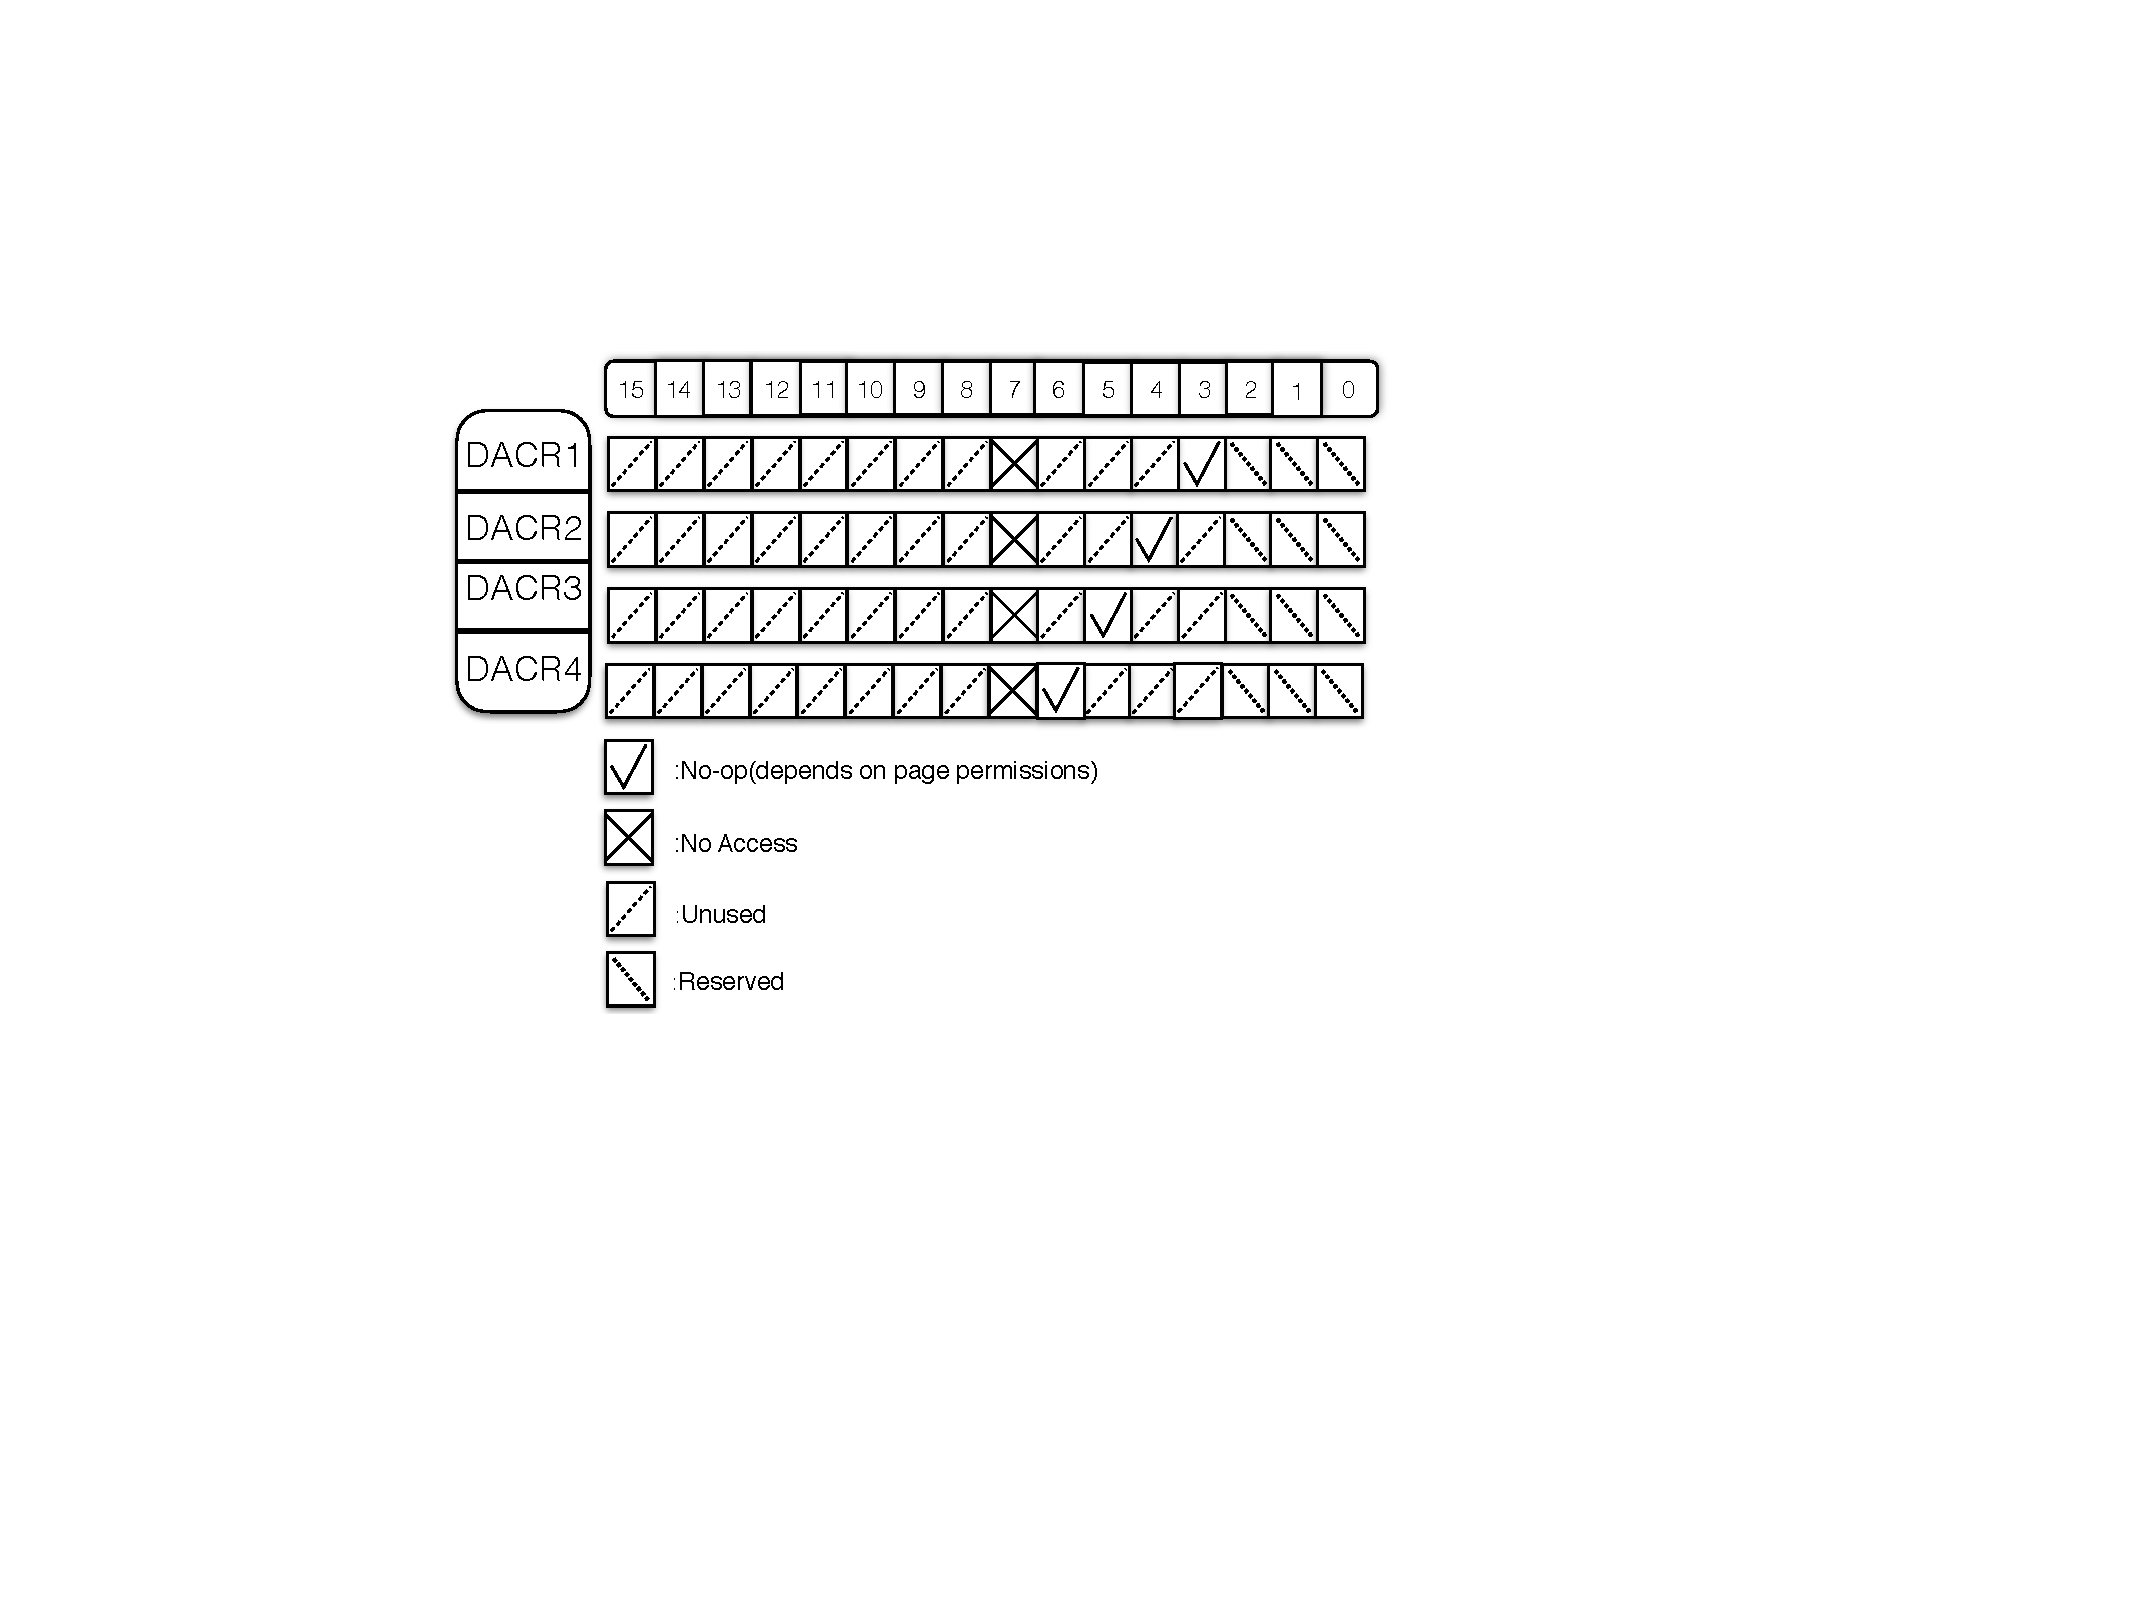
\includegraphics[width=\textwidth]{shreds/figures/dacr}
		\caption{The DACR setup for a quad-core system, where $k=4$. The first 3 domains ($Dom_{0}-Dom_{2}$) are reserved by Linux. Each core has a designated domain ($Dom_{3}-Dom_{6}$) that it may access when executing a shred. No CPU can access $Dom_{7}$. 
		 }
		\label{fig:dacr_setup}
	\end{minipage}
 \hfill
	\begin{minipage}[b]{0.4\textwidth}
		\centering	
		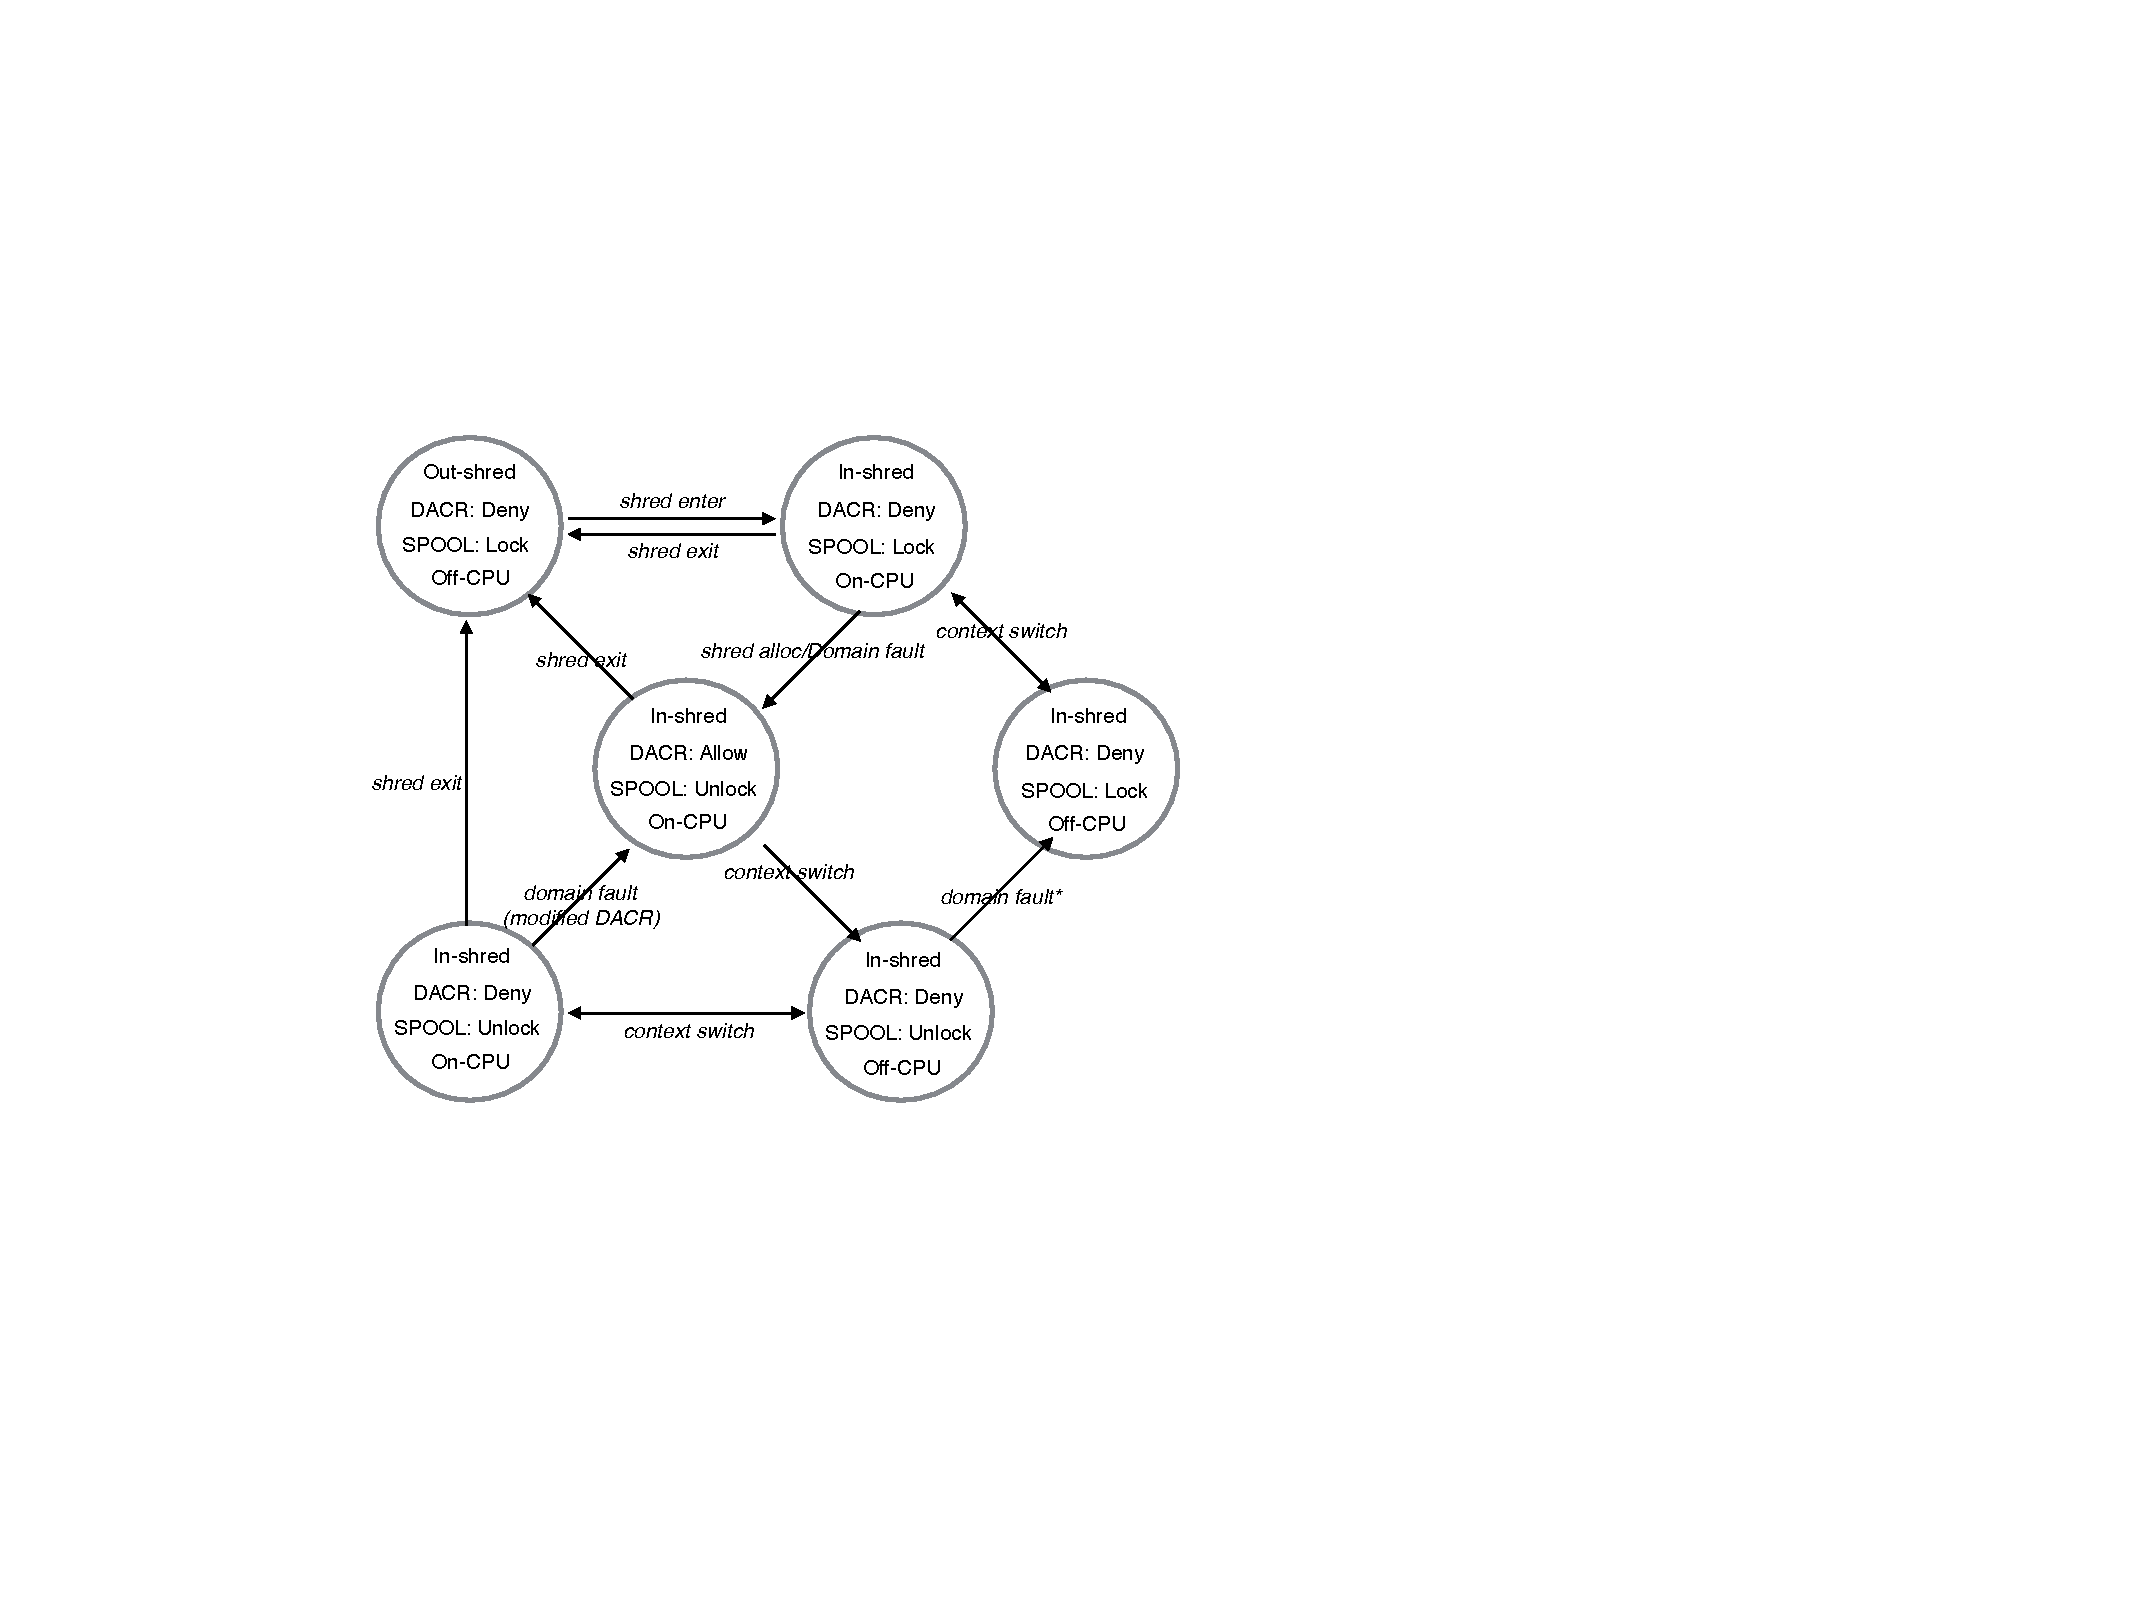
\includegraphics[width=\textwidth]{shreds/figures/shred_state_transition}
		\caption{A shred's transition of states}
		\label{fig:shredstat}
	\end{minipage}
\end{figure*}

S-driver uses the $k$ CPUs and the $k+1$ domains for executing shreds and protecting s-pools. 
When a shred starts or resumes its execution on $CPU_{i}$, S-driver assigns its associated s-pool to $Dom_{i}$, and therefore, the shred can freely access its s-pool while other concurrent threads, if any, cannot. 
When the shred terminates or is preempted, S-driver assigns its s-pool to $Dom_{k+1}$, which prevents any access to the pool from that moment on. 
As a result, S-driver allows or denies access to s-pools on a per-CPU basis, depending on if an associated shred occupies the CPU. 
Even if any malicious code manages to run concurrently alongside the shred inside the same process on another CPU, it cannot access the shred's s-pool without triggering domain faults. Thus, $P1$ is achieved. 

% performance and optimization 
It is reasonably efficient to switch s-pools to different domains upon shred entries and exits are. These operations do not involve heavy page table switches as process- or VM-based solutions do. They only require a shallow walk through of the first level page table and updates to the PDEs pointing to the s-pools in question. Besides, they do not trigger full TLB flushes as our design uses the per-address TLB eviction interface ({\tt flush\_tlb\_page}) and only invalidates the TLB entries related to the updated PDEs. 
To further reduce the overhead, we invent a technique called {\em lazy domain adjustment}: when a shred is leaving $CPU_{i}$, without adjusting any domain assignment, S-driver quickly changes the DACR to revoke the CPU's access to $Dom_{i}$ and lets the CPU's execution continue. It does not assign the s-pool used by the previous shred to $Dom_{k+1}$ until a domain fault happens (\ie another shred coming to the CPU and accessing its s-pool). The lazy domain adjustment avoids unnecessary domain changes and halves the already small overhead in some test cases.

%\begin{figure}[t]
%\begin{center}
%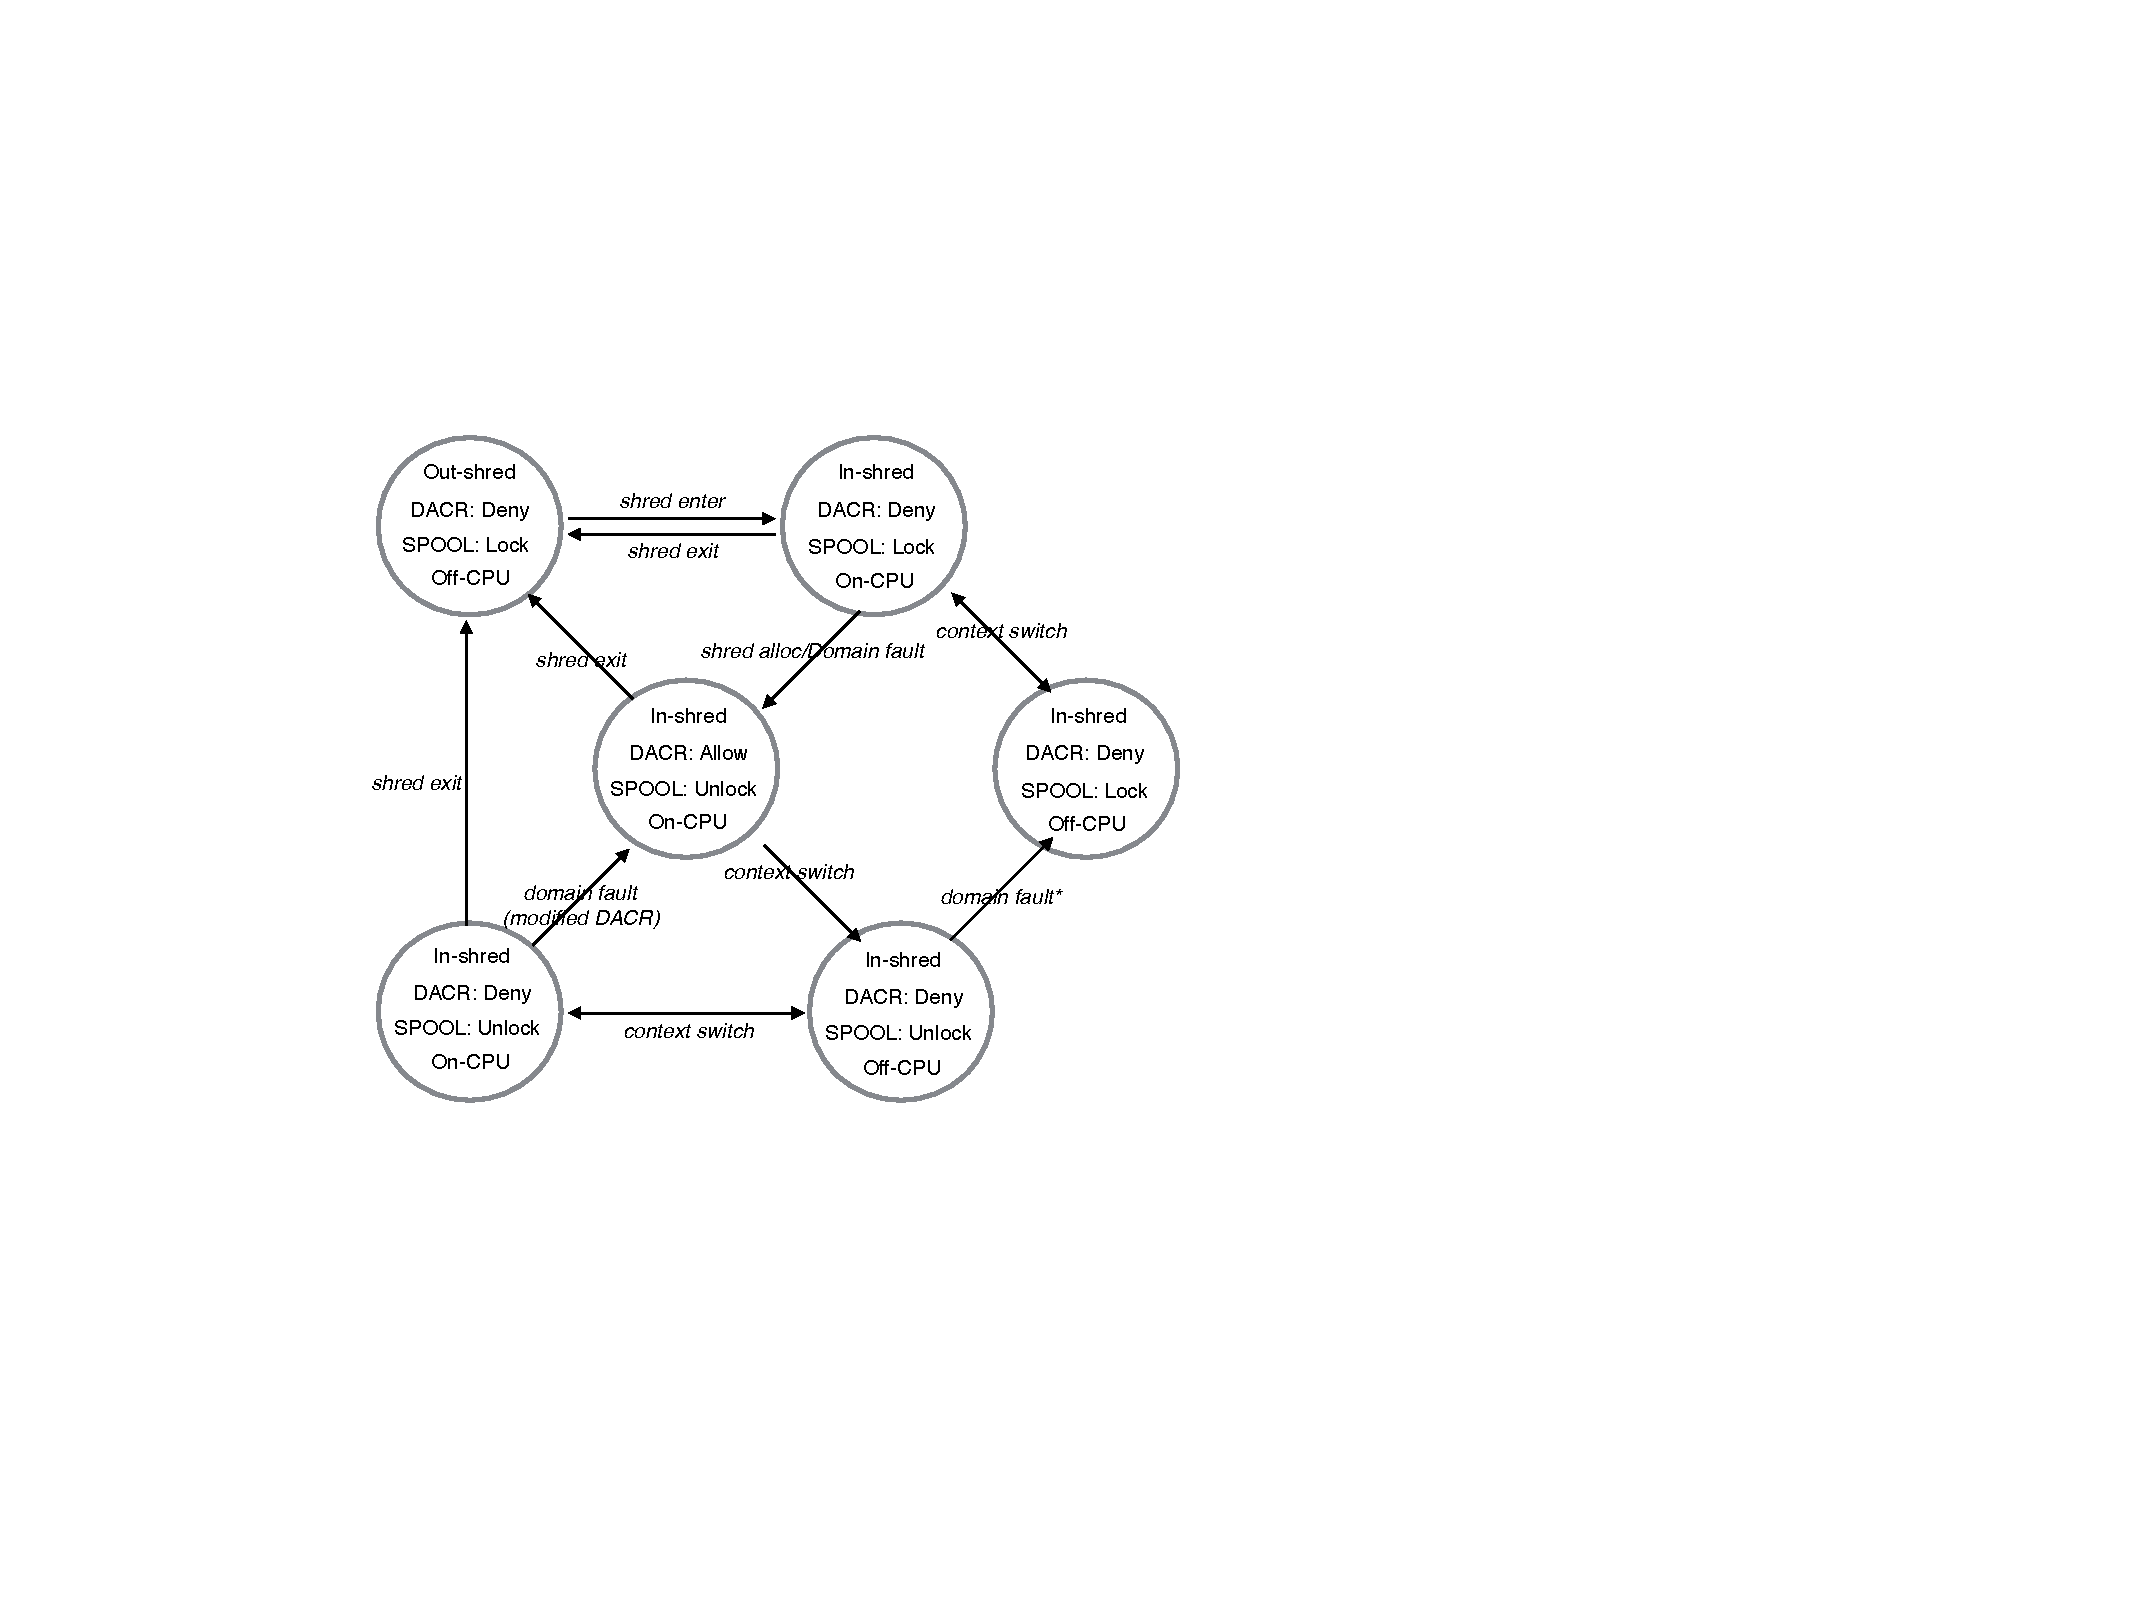
\includegraphics[scale=0.65]{shreds/figures/shred_state_transition}
%\caption{A shred's transition of states}
%\label{fig:shredstat}
%\end{center}
%\end{figure}

Figure~\ref{fig:shredstat} shows how S-driver orchestrates the transitions of a shred's states in response to the API calls, context switches, and domain faults. Each state is defined by a  combination of four properties:  

\begin{itemize}
\item $Shred$ = \{In-shred $|$ Out-shred\}: if the shred has started or exited. 
\item $DACR$ = \{Allow $|$ Deny\}: if the DACR allows or denies the current CPU to access its domain. 
\item $SPOOL$ = \{Lock $|$ Unlock\}: if the associated s-pool is locked or not. 
\item $CPU$ = \{On-CPU $|$ Off-CPU\}: if the shred is running on a CPU or not. 
\end{itemize}

The transition starts from the top, left circle, when the shred has not started and its s-pool is locked. After {\tt shred\_enter} is called, S-driver starts the shred, but it will not adjust the DACR or the s-pool access till a domain fault or a {\tt spool\_alloc} call due to the lazy domain adjustment in effect. When a context switch happens in the middle of the shred execution with unlocked DACR and s-pool, S-driver instantly sets the DACR to Deny but (safely) leaves the s-pool open. Later on, if a domain fault occurs, S-driver locks the previous s-pool because the fault means that the current code running on the CPU is in-shred and is trying to access its s-pool. If a domain fault never occurs till the shred regains the CPU, S-driver does not need to change any domain or s-pool settings, in which case the lazy domain adjustment saves two relatively heavy s-pool locking and unlocking operations. 
 
\point{Secure stacks for shreds}
%shadow stack support and switch 
Although S-compiler forbids unsanitized data flows from s-pools to unprotected memory regions, it has to allow in-shred code to copy s-pool data to local variables, which would be located in the regular stack and potentially accessible to in-process malicious code. 
To prevent secret leaks via stacks, S-driver creates a secure stack for each shred, allocated from its associated s-pool. When code execution enters a shred, S-driver transparently switches the stack without the application's knowledge: it copies the current stack frame to the secure stack and then overwrites the stack pointer. When the shred exits or encounters a signal to be handled outside of the shred, S-driver restores the regular stack.
As a result, local variables used by shreds never exist in regular stacks, and therefore cannot leak secrets.

\point{Runtime protection of shreds}
In addition to enabling and securing shreds and s-pools, S-driver also protects the inline reference monitor (IRM) that S-compiler plants in shred code. 
S-driver write-protects the memory pages containing the instrumented code and the associated data in memory.
It also pins the pages in s-pools in memory to prevent leaks via memory swap.  
Given that our threat model assumes the existence of in-process adversaries, S-driver also mediates the system calls that malicious code in user space may use to overwrite the page protection, dump physical memory via {\tt /dev/*mem}, disturb shreds via {\tt ptrace}, or load untrusted kernel modules. 
For each program using shreds, S-driver starts this mediation before loading the program code, avoiding pre-existing malicious code. 

S-driver's system call mediation also mitigates the attacks that steal secret data, not directly from s-pools, but from the I/O media where secret data are loaded or stored. 
For instance, instead of targeting the private key loaded in an s-pool, an in-process attacker may read the key file on disk. 
S-driver monitors file-open operations insides shreds. When the first time a file $F$ is accessed by a shred $S$, S-driver marks $F$ as a shred-private file and only allows shreds that share the same s-pool with $S$ to access $F$. This restriction is persistent and survives program and system reboots. 
As a result, an attacker can read $F$ only if she manages to intrude the program during its first run and access $F$ before a shred does. Although not completely preventing such attacks, S-driver makes them very difficult to succeed in reality. 
For a complete remedy, we envision a new primitive for in-shred code to encrypt and decrypt secret data with a persistent key assigned to each s-pool and automatically managed by S-driver. However, our current prototype does not support this primitive. 


It is worth noting that, although the system call mediation can prevent user-space malicious code that tries to break shreds via the system interfaces, it is a more intrusive and less configurable design choice than the well-known access control and capability frameworks, such as SELinux, AppArmor, and Capsicum~\cite{watson2010capsicum}. 
However, we leave the integration with those systems as future work because the system call mediation is easy to implement and is sufficient for the prototyping purpose. 



\subsection{Implementation}
\label{shreds:sec:impl}

We built S-compiler based on LLVM~\cite{lattner2004llvm} and its C front-end  Clang~\cite{clang}. We built S-driver with Linux as the reference OS. The implemented system was deployed and evaluated on a quad-core ARM Cortex-A7 computer (Raspberry Pi 2 Model B running Linux 4.1.15).

\point{S-compiler}
The modular and pass-based architecture of LLVM allows us to take advantage of the existing analyzers and easily extends the compilation pipeline. 
S-compiler adds two new passes to LLVM: the shred analysis pass and the security instrumentation pass. Both operate on LLVM bitcode as the IR. 

The analysis pass carries out the checks on the usages and security properties of shreds, as described in \S~\ref{shreds:sec:design}. 
We did not use LLVM's built-in data flow analysis for those checks due to its overly heuristic point-to analysis and the unnecessarily conservative transfer functions.
Instead, we implemented our specialized data flow analysis based on the basic round-robin iterative algorithm, with weak context sensitivity and a straightforward propagation model (i.e., only tracking value-conserving propagators).
We also had to extend LLVM's compilation pipeline because it by default only supports intra-module passes while S-compiler needs to perform inter-module analysis. We employed a linker plugin, called the Link-Time Optimization (LTO), to cross link the IR of all compilation modules and feed the linked IR to our analyzers. 


The instrumentation pass uses the LLVM IR Builder interfaces to insert security checks into the analyzed IR, which are necessary for enforcing the in-shred control flow regulations and preventing dynamic data leaks. 

\IncMargin{1em}
\begin{algorithm}
\small
\SetKwData{Spool}{s\_pool}
\SetKwData{Owner}{s\_owner}
\SetKwData{FaultThread}{fault\_thread}
\SetKwData{CPUDomain}{cpu\_domain}
\SetKwData{SpoolDomain}{s\_pool\_domain}
\SetKwFunction{FindSpool}{FindSpool}
\SetKwFunction{GetOwner}{GetOwner}
\SetKwFunction{GetCPUDomain}{GetCPUDomain}
\SetKwFunction{GetSpoolDomain}{GetSpoolDomain}
\SetKwFunction{BadArea}{bad\_area}
\SetKwFunction{GoodArea}{good\_area}
\SetKwFunction{RestoreDACR}{RestoreDACR}
\SetKwFunction{UnlockSPool}{UnlockSPool}
\SetKwFunction{AdjustSPool}{AdjustSPool}
\SetKwFunction{LockActiveSPoolList}{LockOtherActiveSPools}
\SetKwInOut{Input}{input}
\SetKwInOut{Output}{result}
\Input{The faulting virtual address $fault\_addr$}
\Output{Recover from the domain fault, or kill the faulting thread}
\BlankLine
\emph{/*Identity check*/}\\
  \Spool$\leftarrow$ \FindSpool{$fault\_addr$}\;
  \Owner$\leftarrow$ \GetOwner{$\Spool$}\;
  \If{\FaultThread is NOT in shred}{goto \BadArea}
  \If{\FaultThread is NOT \Owner}{goto \BadArea}
\BlankLine
\emph{/*Recover from domain fault*/}\\
  \CPUDomain$\leftarrow$ \GetCPUDomain{}\;
  \SpoolDomain$\leftarrow$ \GetSpoolDomain{\Spool}\;
   \If{\Spool is unlocked}
   {
   		  
          \If{\CPUDomain $=$ \SpoolDomain}
          {
            \emph{/*No need to change domain for s\_pool*/} \\
            \RestoreDACR{}\;
          }
          \Else
   		  {
   		    \AdjustSPool{\CPUDomain}  
   		  }
   }
    \Else
    {
    	\UnlockSPool{\CPUDomain} 
    }
   \LockActiveSPoolList{\Spool}\;
\caption{Domain Fault Handler}\label{dom_fault_handler}
\end{algorithm}
\DecMargin{1em}

\point{S-driver}
We built S-driver into a Loadable Kernel Module (LKM) for Linux. 
S-driver creates a virtual device file ({\tt /dev/shreds}) to handle the {\tt ioctl} requests made internally by the shred APIs. 
It uses 13 out of 16 memory domains to protect s-pools because the recent versions of Linux kernel for ARM already occupies 3 domains (for isolating device, kernel, and user-space memory). 
S-driver uses the available domains to protect unlimited s-pools and controls each CPU's access to the domains as described in \S~\ref{shreds:sec:design}.
Since Linux does not provide callback interfaces for drivers to react to scheduling events, in order to safely handle context switches or signal dispatches in shreds, 
S-driver dynamically patches the OS scheduler so that, during every context switch, the DACR of the current CPU is reset, which locks the open s-pool, if any. 
The overhead of this operation is negligible because resetting the DACR only takes a single lightweight instruction. 
To capture illegal access to s-pools and lazily adjust domain assignments, 
S-driver registers itself to be the only handler of domain faults and is triggered whenever a domain violation happens. 
Algorithm~\ref{dom_fault_handler} shows how S-driver handles a domain fault. 
Purely implementing S-driver as a LKM allows shreds to be introduced into a host without installing a custom-build kernel image.


\subsection{Analysis}
\label{rpo:sec:analysis}

% \begin{table}[t]
    \caption{Narrowing down the Common Crawl to the candidate set used in our analysis (from left to right).}
    \label{rpo:tab:dataset_stats}
    \centering
    \footnotesize
    \begin{tabular}{lrrr}
    \toprule
    \multicolumn{2}{r}{\textbf{Relative CSS}} & \textbf{Alexa Top 1M} & \textbf{Candidate Set} \\
    \midrule
    All Pages & 203,609,675 & 141,384,967 & 136,793,450 \\
    Tested Pages & 53,725,270 & 31,448,446 & 30,991,702 \\
    Sites & 5,960,505 & 223,212 & 222,443 \\
    Document Types & 9,833 & 2,965 & 2,898 \\
    \bottomrule
    \end{tabular}
\end{table}


For the purposes of our analysis, we gradually narrow down the seed data from
the Common Crawl to pages using relative style paths in the Alexa Top 1\,M,
reflecting injected style directives under RPO, and being exploitable due to
quirks mode rendering.

% Table~\ref{rpo:tab:dataset_stats} shows a summary of our dataset. \textit{Tested
% Pages} refers to the set of randomly selected pages from the page groups as
% discussed in Section~\ref{rpo:sec:methodology:candidate}. For brevity,
% we are referring to \textit{Tested Pages} wherever we mention pages in the
% remainder of the paper.

\subsubsection{Relative Stylesheet Paths}
\label{rpo:sec:analysis:relative}

\begin{figure}[t]
\centering
\begin{minipage}{.32\textwidth}
    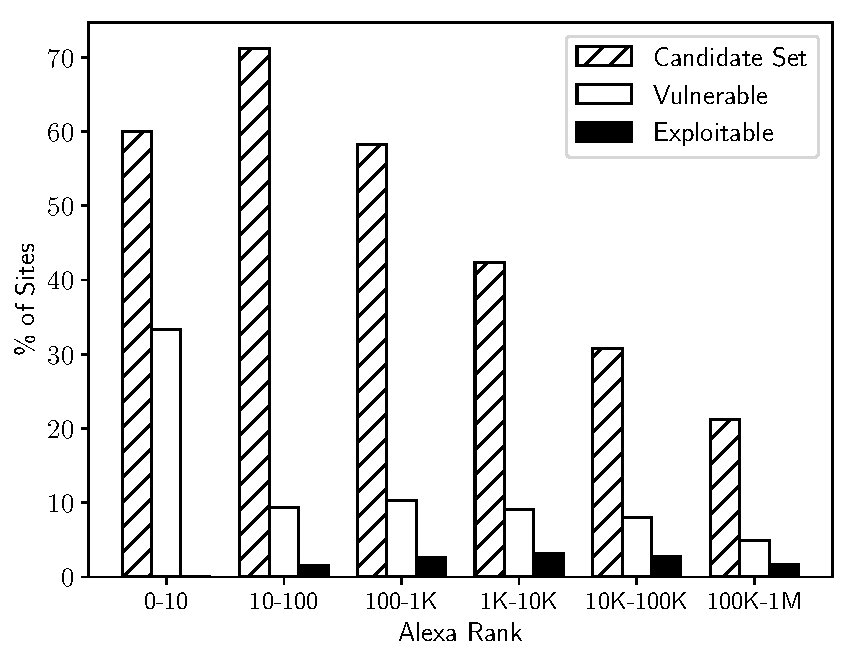
\includegraphics[width=1\textwidth,height=.8\textwidth]{rpo/figures/alexa_rank}
    \caption{Percentage of the Alexa site ranking in our candidate set
             (exponentially increasing bucket size).}
    \label{rpo:fig:analysis:alexa_rank}
\end{minipage}
\hfill
\begin{minipage}{.32\textwidth}
    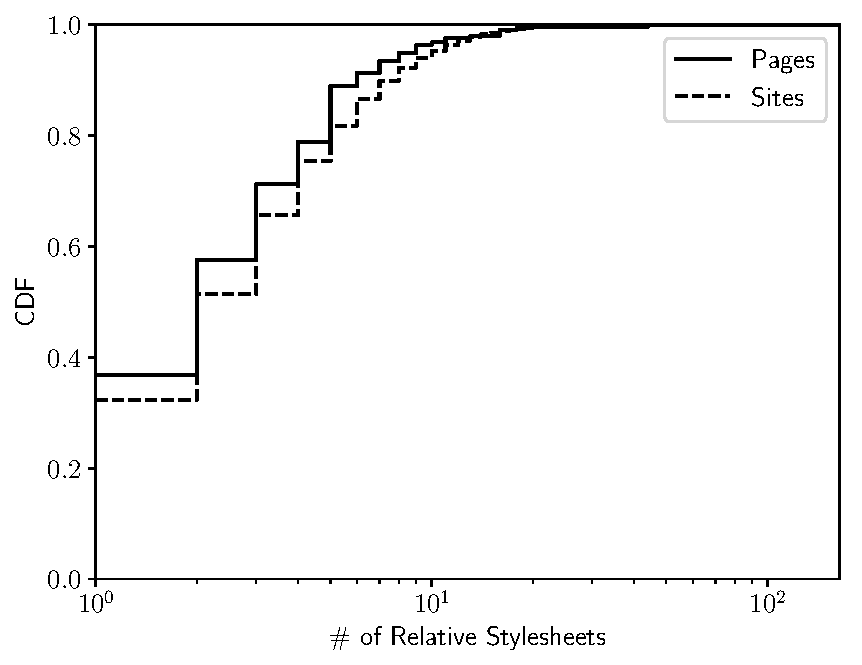
\includegraphics[width=1\textwidth,height=.8\textwidth]{rpo/figures/relative_stylesheets}
    \caption{CDF of total and maximum number of relative stylesheets per web
             page and site, respectively.}
    \label{rpo:fig:analysis:relative_stylesheets}
\end{minipage}
\hfill
\begin{minipage}{.32\textwidth}
    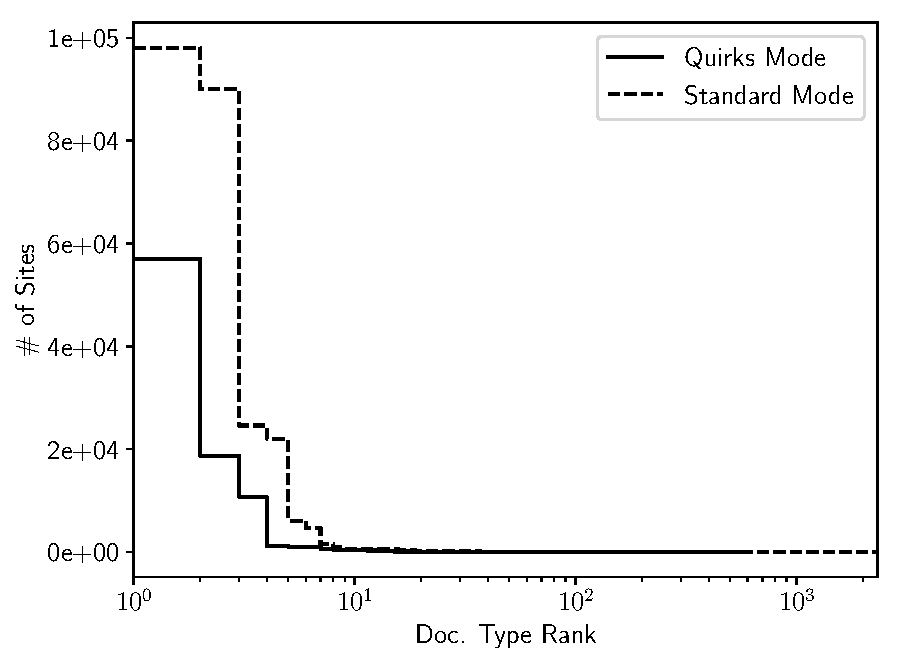
\includegraphics[width=1\textwidth,height=.8\textwidth]{rpo/figures/doctypes_rank_sites}
    \caption{Number of sites containing at least one page with a certain
             document type (ordered by doctype rank).}
    \label{rpo:fig:analysis:doctypes_rank_sites}
\end{minipage}
\end{figure}


To assess the extent to which our Common Crawl-seeded candidate set covers sites
of different popularity, consider the hatched bars in
Figure~\ref{rpo:fig:analysis:alexa_rank}. Six out of the ten largest sites
according to Alexa are represented in our candidate set. That is, they are
contained in the Common Crawl, and have relative style paths. The figure shows
that our candidate set contains a higher fraction of the largest sites and a
lower fraction of the smaller sites. Consequently, our results better represent
the most popular sites, which receive most visitors, and most potential victims
of RPO attacks.

While all the pages in the candidate set contain at least one relative
stylesheet path, Figure~\ref{rpo:fig:analysis:relative_stylesheets} shows that
63.1\,\% of them contain multiple relative paths, which increases the chances of
finding a successful RPO and style injection point.

\subsubsection{Vulnerable Pages}
\label{rpo:sec:analysis:vulnerable}

\begin{table*}[t]
    \centering
    \caption{Vulnerable/exploitable pages and sites in the candidate set (IE using framing).}
    \label{rpo:tab:vulnerable_exploitable_result}
    \footnotesize
    \begin{tabular}{lrrrrrr}
    \toprule
    \multirow{2}{*}{\textbf{Technique}} &
    \multicolumn{2}{c}{\textbf{Vulnerable}} &
    \multicolumn{2}{c}{\textbf{Exploitable (Chrome)}} &
    \multicolumn{2}{c}{\textbf{Exploitable (IE)}} \\

    \cmidrule[0.5pt](lr){2-3}
    \cmidrule[0.5pt](lr){4-5}
    \cmidrule[0.5pt](lr){6-7}

    &
    \textbf{Pages} &
    \textbf{Sites} &
    \textbf{Pages} &
    \textbf{Sites} &
    \textbf{Pages} &
    \textbf{Sites}
    \\

    \midrule

    Path Parameter & 309,079 (1.0\%) & 9,136 (4.1\%) & 6,048 (\textless 0.1\%) & 1,025 (0.5\%) & 52,344 (0.2\%) & 3,433 (1.5\%) \\
    Encoded Path & 53,502 (0.2\%) & 1,802 (0.8\%) & 3 (\textless 0.1\%) & 2 (\textless 0.1\%) & 24 (\textless 0.1\%) & 5 (\textless 0.1\%) \\
    Encoded Query & 89,757 (0.3\%) & 1,303 (0.6\%) & 23 (\textless 0.1\%) & 20 (\textless 0.1\%) & 137 (\textless 0.1\%) & 43 (\textless 0.1\%) \\
    Cookie & 15,656 (\textless 0.1\%) & 1,030 (0.5\%) & 4,722 (\textless 0.1\%) & 81 (\textless 0.1\%) & 2,447 (\textless 0.1\%) & 238 (0.1\%) \\

    \midrule

    Total & 377,043 (1.2\%) & 11,986 (5.4\%) & 10,781 (<0.1\%) & 1,106 (0.5\%) & 54,853 (0.2\%) & 3,645 (1.6\%) \\

    \bottomrule
    \end{tabular}

\end{table*}


We consider a candidate page vulnerable if one of the style injection techniques
of Section~\ref{rpo:sec:methodology:vulnerable} succeeds. In other
words, the server's response should reflect the injected payload. Furthermore,
we conservatively require that the response not contain a \texttt{base} tag
since a correctly configured base tag can prevent path confusion.

Table~\ref{rpo:tab:vulnerable_exploitable_result} shows that 1.2\,\% of pages
are vulnerable to at least one of the injection techniques, and 5.4\,\% of sites
contain at least one vulnerable page. The path parameter technique is most
effective against pages, followed by the encoded query and the encoded path
techniques. Sites that are ranked higher according to Alexa are more likely to
be vulnerable, as shown in Figure~\ref{rpo:fig:analysis:alexa_rank}, where
vulnerable and exploitable sites are relative to the candidate set in each
bucket. While one third of the candidate set in the Top~10 (two out of six
sites) is vulnerable, the percentage oscillates between 8 and 10\,\% among the
Top~100\,k. The candidate set is dominated by the smaller sites in the ranks
between 100\,k and 1\,M, which have a vulnerability rate of 4.9\,\% and push
down the average over the entire ranking.

% A \texttt{base} tag in the server response can prevent path confusion because it
% indicates how the browser should expand relative paths. We observed a number of
% inconsistencies with respect to its use. At first, 603 pages on 60 sites
% contained a \texttt{base} tag in their response; however, the server response
% after injecting our payload did not contain the tag anymore, rendering these
% pages potentially exploitable. Furthermore, Internet Explorer's implementation
% of the \texttt{base} tag appears to be broken. When such a tag is present,
% Internet Explorer fetches two URLs for stylesheets---one expanded according to
% the base URL specified in the tag, and one expanded in the regular, potentially
% ``confused'' way of using the page URL as the base. In our experiments, Internet
% Explorer always applied the ``confused'' stylesheet, even when the one based on
% the \texttt{base} tag URL loaded faster. Consequently, \texttt{base} tags do not
% appear to be an effective defense against RPO in Internet Explorer (They seem to
% work as expected in other browsers, including Edge).


\subsubsection{Exploitable Pages}
\label{rpo:sec:analysis:exploitable}

To test whether a vulnerable page was exploitable, we opened it in Chrome,
injected a style payload with an image reference (randomly generated URL), and
checked if the image was indeed loaded. This test succeeded for 2.9\,\% of
vulnerable pages; 0.5\,\% of sites in the candidate set had at least one
exploitable page (Table~\ref{rpo:tab:vulnerable_exploitable_result}).

% In the following, we explore various factors that may impact whether a
% vulnerable page can be exploited, and we show how some of these partial defenses
% can be bypassed.

% \paragraph{Document Types}
% \label{rpo:sec:analysis:doctypes}

% \begin{table}[t]
\centering
\begin{minipage}[t]{.55\textwidth}
    \caption{Summary of document type usage in sites.\newline}
    \label{rpo:tab:doctypes_summary}
    \centering
    \footnotesize
    \begin{tabular}{lrr}
    \toprule
    \textbf{Doc. Type} & \textbf{At Least One Page} & \textbf{All Pages} \\
    \midrule

    None & 56,985 (25.6\%) & 19,968 (9.0\%) \\
    Quirks & 27,794 (12.5\%) & 7,720 (3.5\%) \\
    None or Quirks & 71,597 (32.2\%) & 30,040 (13.5\%) \\
    \addlinespace
    Standards & 192,403 (86.5\%) & 150,846 (67.8\%) \\    
    \bottomrule
    \end{tabular}
\end{minipage}
\hfill
\begin{minipage}[t]{.43\textwidth}
    \caption{Quirks mode document types by browser.}
    \label{rpo:tab:doctypes_browsers}
    \centering
    \footnotesize
    \begin{tabular}{llr}
    \toprule

    \textbf{Browser} &
    \textbf{OS} &
    \textbf{Doc. Types} \\

    \midrule
    Chrome 55 & Linux & 1,378 (31.9\,\%) \\
    Opera 42 & Linux & 1,378 (31.9\,\%) \\
    Safari 10 & macOS & 1,378 (31.9\,\%) \\
    \addlinespace
    Firefox 50 & Linux & 1,326 (30.7\,\%) \\
    \addlinespace
    Edge 38 & Windows & 1,319 (30.5\,\%) \\
    IE 11 & Windows & 1,319 (30.5\,\%) \\
    \bottomrule
    \end{tabular}
\end{minipage}
\end{table}


% \begin{table}[t]
    \caption{Most frequent document types causing all browsers to render
    in quirks mode, as well as the sites that use at least one such
    document type.}
    \label{rpo:tab:top_quirksmode_doctypes}
    \centering
    \footnotesize
    \begin{tabular}{lrr}
    \toprule
    \textbf{Document Type (shortened)} & \textbf{Pages} & \textbf{Sites} \\
    \midrule
    (none) & 1,818,595 (5.9\,\%) & 56,985 (25.6\,\%) \\
    "-//W3C//DTD HTML 4.01 Transitional//EN" & 721,884 (2.3\,\%) & 18,648 (8.4\,\%) \\
    "-//W3C//DTD HTML 4.0 Transitional//EN" & 385,656 (1.2\,\%) & 11,566 (5.2\,\%) \\
    "-//W3C//DTD HTML 3.2 Final//EN" & 22,019 (<0.1\,\%) & 1,175 (0.5\,\%) \\
    "-//W3C//DTD HTML 3.2//EN" & 10,839 (<0.1\,\%) & 927 (0.4\,\%) \\
    \midrule
    All & 3,046,449 (9.6\,\%) & 71,597 (32.2\,\%) \\
    \bottomrule
    \end{tabular}
\end{table}


% HTML document types play a significant role in RPO-based style injection attacks
% because browsers typically parse resources with a non-CSS content type in a CSS
% context only when the page specifies an ancient or non-standard HTML document
% type (or none at all). The pages in our candidate set contain a total of 4,318
% distinct document types. However, the majority of these unique document types
% are not standardized and differ from the standardized ones only by small
% variations, such as forgotten spaces or misspellings.

% To determine how browsers interpret these document types (i.e., whether they
% cause them to render a page in standards or quirks mode), we designed a
% controlled experiment. For each unique document type, we set up a local page
% with a relative stylesheet path and carried out an RPO attack to inject CSS
% using a payload similar to what we described in
% Section~\ref{rpo:sec:methodology:vulnerable}. We automatically opened
% the local page in Chrome, Firefox, Edge, Internet Explorer, Safari, and Opera,
% and we kept track of which document type caused the injected CSS to be parsed
% and the injected background image to be downloaded.

% Table~\ref{rpo:tab:doctypes_browsers} contains the results of this experiment.
% Even though the exact numbers vary among browsers, roughly a third of the unique
% document types we encountered result in quirks mode rendering. Not surprisingly,
% both Microsoft products Edge and Internet Explorer exhibit identical results,
% whereas the common Webkit ancestry of Chrome, Opera, and Safari also show
% identical results. Overall, 1,271 (29.4\,\%) of the unique document types force
% all the browsers into quirks mode, whereas 1,378 (31.9\,\%) of them cause at
% least one browser to use quirks mode rendering.
% Table~\ref{rpo:tab:top_quirksmode_doctypes} shows the most frequently used
% document types that force all the browsers into quirks mode, which includes the
% absence of a document type declaration in the page.

% To test how often Internet Explorer allows a page's document type to be
% overridden when loading it in an \texttt{iframe}, we created another controlled
% experiment using a local attack page framing the victim page, as outlined in
% Section~\ref{rpo:sec:methodology:exploitable}. Using Internet
% Explorer~11, we loaded our local attack page for each unique document type
% inside the frame, and tested if the injected CSS was parsed. While Internet
% Explorer parsed the injected CSS for 1,319 (30.5\,\%) of the document types in
% the default setting, the frame override trick caused CSS parsing for 4,248
% (98.4\,\%) of the unique document types.

% While over one thousand document types result in quirks mode, and around three
% thousand document types cause standards mode parsing, the number of document
% types that have been standardized is several orders of magnitude smaller. In
% fact, only a few (standardized) document types are used frequently in pages,
% whereas the majority of unique document types are used very rarely.
% Figure~\ref{rpo:fig:analysis:doctypes_rank_sites} shows that only about ten
% standards and quirks mode document types are widely used in pages and sites.
% Furthermore, only about 9.6\,\% of pages in the candidate set use a quirks mode
% document type; on the remaining pages, potential RPO style injection
% vulnerabilities cannot be exploited because the CSS would not be parsed (unless
% Internet Explorer is used). However, when grouping pages in the candidate set by
% site, 32.2\,\% of sites contain at least one page rendered in quirks mode
% (Table~\ref{rpo:tab:doctypes_summary}), which is one of the preconditions for
% successful RPO.

% \paragraph{Internet Explorer Framing}

% We showed above that by loading a page in a frame, Internet Explorer can be
% forced to disregard a standards mode document type that would prevent
% interpretation of injected style. To find out how often this technique can be
% applied for successful RPO attacks, we replicated our Chrome experiment in
% Internet Explorer, this time loading each vulnerable page inside a frame. Around
% 14.5\,\% of vulnerable pages were exploitable in Internet Explorer, five times
% more than in Chrome (1.6\,\% of the sites in the candidate set).

% Figure~\ref{rpo:fig:analysis:alexa_rank} shows the combined exploitability
% results for Chrome and Internet Explorer according to the rank of the site.
% While our methodology did not find any exploitable vulnerability on the six
% highest-ranked sites in the candidate set, between 1.6\,\% and 3.2\,\% of
% candidate sites in each remaining bucket were found to be exploitable. The
% highest exploitability rate occurred in the ranks 1\,k through 10\,k.

% Broken down by injection technique, the framing trick in Internet Explorer
% results in more exploitable pages for each technique except for cookie injection
% (Table~\ref{rpo:tab:vulnerable_exploitable_result}). One possible explanation
% for this difference is that the Internet Explorer crawl was conducted one month
% after the Chrome crawl, and sites may have changed in the meantime. Furthermore,
% we observed two additional impediments to successful exploitation in Internet
% Explorer that do not apply to Chrome. The framing technique is susceptible to
% frame-busting methods employed by the framed pages, and Internet Explorer
% implements an anti-MIME-sniffing header that Chrome appears to ignore. We
% analyze these issues below.

% \paragraph{Anti-Framing Techniques}

% Some sites use a range of techniques to prevent other pages from loading them in
% a frame~\cite{w2sp2010frame_busting}. One of these techniques is the
% \texttt{X-Frame-Options} header. It accepts three different values:
% \texttt{DENY}, \texttt{SAMEORIGIN}, and \texttt{ALLOW-FROM} followed by a
% whitelist of URLs.

% In the vulnerable dataset, 4,999 pages across 391 sites use this header
% correctly and as a result prevent the attack. However, 1,900 pages across 34
% sites provide incorrect values for this header, and we successfully attack 552
% pages on 2 sites with Internet Explorer.

% A related technique is the \texttt{frame-ancestors} directive provided by
% Content Security Policy. It defines a (potentially empty) whitelist of URLs
% allowed to load the current page in a frame, similar to \texttt{ALLOW-FROM}.
% However, it is not supported by Internet Explorer, thus it cannot be used to
% prevent the attack.

% Furthermore, developers may use JavaScript code to prevent framing of a page.
% Yet, techniques exist to bypass this
% protection~\cite{owasp_clickjacking_defence}. In addition, the attacker can use
% the HTML 5 \texttt{sandbox} attribute in the \texttt{iframe} tag and omit the
% \texttt{allow-top-navigation} directive to render JavaScript frame-busting code
% ineffective. However, we did not implement any of these techniques to allow
% framing, which means that more vulnerable pages could likely be exploited in
% practice.

% \paragraph{MIME Sniffing}

% A consequence of self-reference in the type of RPO studied in this paper is that
% the HTTP content type of the fake ``stylesheet'' is \texttt{text/html} rather
% than the expected \texttt{text/css}. Because many sites contain misconfigured
% content types, many browsers attempt to infer the type based on the request
% context or file extension (\textit{MIME sniffing}), especially in quirks mode.
% In order to ask the browser to disable content sniffing and refuse interpreting
% data with an unexpected or wrong type, sites can set the header
% \texttt{X-Content-Type-Options: nosniff}~\cite{sp2009contentsniff,firefox_mime_sniff,content_type_options}.

% To determine whether the injected CSS is still being parsed and executed in
% presence of this header while the browser renders in quirks mode, we ran an
% experiment similar to Section~\ref{rpo:sec:analysis:doctypes}. For each browser
% in Table~\ref{rpo:tab:doctypes_browsers}, we extracted the document types in
% which the browser renders in quirks mode, and for each of them, we set up a
% local page with a relative stylesheet path. We then opened the page in the
% browser, launched an RPO attack, and monitored if the injected CSS was executed.

% Only Firefox, Internet Explorer, and Edge respected this header and did not
% interpret injected CSS in any of the quirks mode document types. The remaining
% browsers did not block the stylesheet even though the content type was not
% \texttt{text/css}. With an additional experiment, we confirmed that Internet
% Explorer blocked our injected CSS payload when \texttt{nosniff} was set, even in
% the case of the framing technique.

% Out of all the vulnerable pages, 96,618 pages across 232 sites had a
% \texttt{nosniff} response header; 23 pages across 10 sites were confirmed
% exploitable in Chrome but not in Internet Explorer, since the latter browser
% respects the header while the former does not.

% \subsubsection{Content Management Systems}
% \label{rpo:sec:analysis:cmses}

% While analyzing the exploitable pages in our dataset, we noticed that many
% appeared to belong to well-known CMSes. Since these web applications are
% typically installed on thousands of sites, fixing RPO weaknesses in these
% applications could have a large impact.

% To identify CMSes, we visited all exploitable pages using
% Wappalyzer~\cite{wappalyzer}. Additionally, we detected two CMSes that were not
% supported by Wappalyzer. Overall, we identified 23 CMSes on 41,288 pages across
% 1,589 sites. Afterwards, we manually investigated whether the RPO weakness
% stemmed from the CMS by installing the latest version of each CMS (or using the
% online demo), and testing whether exploitable paths found in our dataset were
% also exploitable in the CMS. After careful analysis, we confirmed four CMSes to
% be exploitable in their most recent version that are being used by 40,255 pages
% across 1,197 sites.

% Out of the four exploitable CMSes, one declares no document type and one uses a
% quirks mode document type. These two CMSes can be exploited in Chrome, whereas
% the remaining two can be exploited with the framing trick in Internet Explorer.
% % Beyond the view of our Common Crawl candidate set, Wappalyzer detected nearly
% % 32\,k installations of these CMSes across the Internet, which suggests that many
% % more sites could be attacked with RPO. We reported the RPO weaknesses to the
% % vendors of these CMSes using recommended notification
% % techniques~\cite{usenixsec2016vulnnotify1,usenixsec2016vulnnotify2,weis2017vulnnotify}.
% % Thus far, we heard back from one of the vendors, who acknowledged the
% % vulnerability and are going to take the necessary steps to fix the issue.
% % However, we have not received any response from the other vendors.

% \subsubsection{Mitigation Techniques}
% \label{rpo:sec:mitigation}

% Relative path overwrites rely on the web server and the web browser interpreting
% URLs differently. HTML pages can use only absolute (or root-relative) URLs,
% which removes the need for the web browser to expand relative paths.
% Alternatively, when the HTML page contains a \texttt{<base>} tag, browsers are
% expected to use the URL provided therein to expand relative paths instead of
% interpreting the current document's URL.
% % Both methods can remove ambiguities and
% % render RPO impossible if applied correctly. Specifically, base URLs must be set
% % according to the server's content routing logic. If developers choose to
% % calculate base URLs dynamically on the server side rather than setting them
% % manually to constant values, there is a risk that routing-agnostic algorithms
% % could be confused by manipulated URLs and re-introduce attack opportunities by
% % instructing browsers to use an attacker-controlled base URL. Furthermore,
% % Internet Explorer does not appear to implement this tag correctly.
% % 
% Web developers can reduce the attack surface of their sites by eliminating any
% injection sinks for strings that could be interpreted as a style directive.
% % However, doing so is challenging because in the attack presented in this paper,
% % style injection does not require a specific sink type and does not need the
% % ability of injecting markup. Injection can be accomplished with relatively
% % commonly used characters, that is, alphanumeric characters and
% % \texttt{()\{\}/"}. Experience has shown that despite years of efforts, even
% % context-sensitive and more special character-intensive XSS injection is still
% % possible in many sites, which leads us to believe that style injection will be
% % similarly difficult to eradicate. Even when all special characters in user input
% % are replaced by their corresponding HTML entities and direct style injection is
% % not possible, more targeted RPO attack variants referencing existing files may
% % still be feasible. For instance, it has been shown that user uploads of
% % seemingly benign profile pictures can be used as ``scripts'' (or
% % stylesheets)~\cite{rpo_techniques}.

% Instead of preventing RPO and style injection vulnerabilities, the most
% promising approach could be to avoid exploitation. In fact, declaring a modern
% document type that causes the HTML document to be rendered in standards mode
% makes the attack fail in all browsers except for Internet Explorer. Web
% developers can harden their pages against the frame-override technique in
% Internet Explorer by using commonly recommended HTTP headers.
% % \texttt{X-Content-Type-Options} to disable ``content type sniffing'' and always
% % use the MIME type sent by the server (which must be configured correctly),
% % \texttt{X-Frame-Options} to disallow loading the page in a frame, and
% % \texttt{X-UA-Compatible} to turn off Internet Explorer's compatibility view.


\section{Milestones}

The plan for completing my research is presented in Table~\ref{tab:milestones}.

\begin{table}[h]
    \caption{Plan for completion}
    \label{tab:milestones}
    \centering
    \footnotesize
    \begin{tabular}{lr}
    \toprule
    \textbf{Task} & \textbf{Completion Date} \\
    \midrule
    Complete Implementation of \savior & March 2019 \\
    Evaluate \savior on large real-world programs & April 2019 \\
    Finalizing \savior for publication & June 2019 \\
    Explore Summarization Rules for UaF bugs & July 2019 \\
    Dissertation defense & September 2019 \\
    \bottomrule
    \end{tabular}
\end{table}
%\clearpage


\pagebreak

\footnotesize
\bibliographystyle{plain}
\bibliography{proposal}

\end{document}
